\chapter{Contexte physique}

L'objectif de ce chapitre est de pr\'esenter le contexte g\'en\'eral de la th\`ese. Pour cela, nous allons pr\'esenter le contexte th\'eorique et exp\'erimental de la physique \`a l'origine de cette th\`ese. Nous présenterons dans une première section le mod\`ele standard de la physique des particules puis nous en décrirons les limitations. Nous d\'ecrirons ensuite diff\'erentes nouvelles th\'eories qui permettent de d\'epasser le mod\`ele standard. Dans une seconde partie, nous d\'ecrirons une partie les dispositifs exp\'erimentaux utilis\'es en physique : les acc\'el\'erateurs de particules. Nous dresserons alors le portrait des diff\'erents types de collisionneurs de particules et nous exposerons quelques unes des derni\`eres d\'ecouvertes r\'ealis\'ees en physique des particules ces vingt derni\`eres ann\'ees. Enfin, nous parlerons des collisionneurs du futur, et nous mettrons l'accent sur l'ILC. Nous en analyserons les d\'etecteurs et notamment le d\'etecteur de vertex envisag\'e pour l'ILD puisque cette th\`ese prend naissance dans le contexte du d\'etecteur de vertex pour l'ILD bas\'e sur les capteurs CMOS d\'evelopp\'es par le groupe \textit{PICSEL}.

% Mod\`ele standard \\
% EW \\
% Brisure : Higgs \\
% Contexte exp\'erimentale \\
% Collisionneurs \\
% ILC \\
% Physique \`a l'ILC \\
% D\'etecteur de vertex de l'ILD. \\
% COntraintes sur le detecteur de vertex pour l'ILD et proposition d'une g\'eom\'etrie \\
% Alignement et AIDA \\

\section{Mod\`ele standard}

Nous allons pr\'esenter dans cette partie le contexte th\'eorique de la physique des particules. Pour cela nous ferons une revue non exhaustive du mod\`ele standard de la physique des particules puis nous d\'ecrirons quelques unes de ces limitations. Enfin nous pr\'esenterons quelques th\'eories permettant de r\'esoudre certaines de ces limitations et de franchir un nouveau pas vers la description du monde physique.  

\subsection{G\'en\'eralit\'es}

\begin{figure}[htb!]
 \begin{center}
   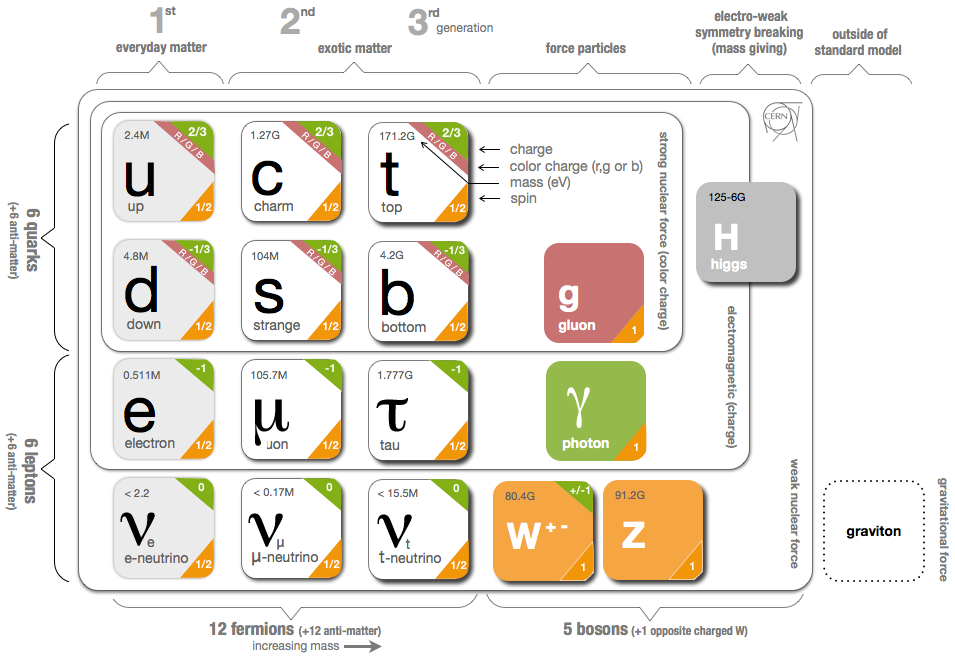
\includegraphics[scale=0.40]{./figures/Standard_model_infographic.png}
   \caption{Représentation des particules du mod\`ele standard de la physique des particules.}
  \end{center}
\end{figure}

Le mod\`ele standard de la physique des particules est la th\'eorie qui r\'egit 
les interactions entre les particules qui constituent la mati\`ere. 
Il d\'ecrit les particules fondamentales qui composent la mati\`ere : les 
fermions et les particules qui v\'ehiculent 3 des 4 forces fondamentales qui 
gouvernent la nature : les bosons. En effet, la gravitation n'est pas d\'ecrite 
par le mod\`ele standard.

\medskip

Une repr\'esentation du mod\`ele standard est la suivante : dans ce mod\`ele les fermions, particules de spin demi-entiers, sont au nombre de 12 ; et les bosons, particules de spin entiers sont aussi au nombre de 12.
La famille des fermions se d\'ecompose en 2 sous ensembles, les quarks d'une 
part, et les leptons, d'autres part. 

\medskip

Les quarks sont des particules de spin $\frac{1}{2}$ et ils poss\`edent une 
charge fractionnaire de la charge \'el\'ementaire. Ils sont r\'epartis en 3 familles 
appel\'ees g\'en\'erations. Les quarks sont au nombre de 6 et se distinguent par leur 
masse et leur charge \'electrique. Leurs noms autrement appel\'es saveurs sont list\'es dans le 
tableau \ref{tab:quarks}.

\begin{table}[h]
\begin{center}
\begin{tabular}[t]{|l|l|l|l|} \hline
        & $1^{\text{\`ere}}$ g\'en\'eration & $2^{\text{nde}}$ g\'en\'eration         & $3^{\text{\`eme}}$ g\'en\'eration     \\ \hline
 Quarks & \textbf{u} \textit{up} (haut)     & \textbf{c} \textit{charm} (charm\'e)    & \textbf{t} \textit{top} (v\'erit\'e)  \\
        & \textbf{d} \textit{down} (bas)    & \textbf{s} \textit{strange} (\'etrange) & \textbf{b} \textit{bottom} (beaut\'e) \\ \hline
\end{tabular}
\caption{Quarks du mod\`ele standard.}
\label{tab:quarks}
\end{center}
\end{table}

\medskip

Les leptons, sont des particules de spin $\frac{1}{2}$. \`A la diff\'erence des 
quarks, ils ne sont pas sensibles \`a l'interaction forte. Dans le mod\`ele standard, seule 
l'interaction électrofaible les gouverne. Ils sont r\'epartis en 3 doublets d'isospin faible. Chaque doublet est compos\'e d'une particule ayant le nom de sa saveur et d'un neutrino. Ces 3 doublets sont 
expos\'es dans le tableau \ref{tab:leptons}.

\begin{table}[h]
\begin{center}
\begin{tabular}[t]{|l|l|l|l|} \hline
         & $1^{\text{\`ere}}$ g\'en\'eration & $2^{\text{nde}}$ g\'en\'eration & $3^{\text{\`eme}}$ g\'en\'eration \\ \hline
         & $\mathbf{e^-}$ électron           & $\mathbf{\mu^-}$ muon           & $\mathbf{\tau^-}$ tau             \\
 Leptons & $\mathbf{\nu_e}$ neutrino         & $\mathbf{\nu_{\mu}}$ neutrino   & $\mathbf{\nu_{\tau}}$ neutrino    \\
         & \'electronique                    & muonique                        & tauique                           \\ \hline
\end{tabular}
\caption{Leptons du mod\`eles standard.}
\label{tab:leptons}
\end{center}
\end{table}

\medskip

Les bosons de jauges sont des particules de spin 1. Ils sont les vecteurs des 3 
interactions fondamentales d\'ecrites par le mod\`ele standard. Une revue des 
bosons de jauge est faite dans le tableau \ref{tab:bosons}. 

\begin{table}[h]
\begin{center}
\begin{tabular}[t]{|l|l|l|l|} \hline
 Interaction & \'Electromagn\'etique & Faible          & Forte    \\ \hline
 Boson       & $\gamma$ Photon     & $W^+, W^-, Z^0$ & 8 Gluons \\ \hline
\end{tabular}
\caption{Interactions et bosons correspondant du mod\`ele standard.}
\label{tab:bosons}
\end{center}
\end{table}

\medskip

La derni\`ere pierre \`a l'\'edifice du mod\`ele standard est le Boson de 
Higgs. Il permet de briser spontan\'ement l'interaction \'electrofaible et 
donne leurs masses aux particules. Nous reviendrons plus loin dans ce chapitre 
sur ce boson. Une fois ces g\'en\'eralit\'es ph\'enom\`enologique d\'ecrites, voyons plus en d\'etail la th\'eorie du mod\`ele standard.

%12 fermions spins demi-entiers
%12 bosons spins entiers
%-> mettre un tableau.
%mesons = quark + antiquark
%barions : 3 quarks

\subsection{Th\'eorie}

Le mod\`ele standard est une th\'eorie invariante de jauge par le groupe de jauge suivant : 

\begin{equation} 
   SU_C(3) \otimes SU_L(2) \otimes U_Y(1) 
\end{equation}

$SU_C(3)$ est le groupe de sym\'etrie associ\'e \`a l'interaction forte. 
Cette interaction est v\'ehicul\'ee par 8 bosons de jauges appel\'es gluons. 
L'indice $_C$ indique que seules les particules poss\'edant une charge de 
couleurs interagissent par le biais de l'interaction forte. Ainsi, seuls les 
quarks et les gluons sont sensibles \`a cette interaction. Nous ne nous attarderons pas plus sur cette interaction. 

\medskip

$SU_L(2) \otimes U_Y(1)$ est le groupe de sym\'etrie de l'interaction 
\'electrofaible. Il s'agit de l'unification des forces \'electromagn\'etiques et 
faibles. L'interaction faible est transmise par les bosons de jauges $W^-, W+$ 
et $Z^0$. Le vecteur de l'interaction \'electromagn\'etique est quant \`a lui 
le photon $\gamma$. L'indice L pour $Left$ signifie que seules les particules 
de chiralit\'e gauche interagissent par l'interaction faible. L'indice Y 
quant \`a lui se r\'ef\`ere \`a l'hypercharge.
La relation entre la charge et l'hypercharge, dite relation de \textit{Gell-Mann 
Nishijima} est la suivante :
 
\[ \cfrac{Y}{2} = Q - T^3 \]

O\`u Y est l'hypercharge, Q la charge \'electrique et $T^3$ la troisi\`eme 
composante de l'isospin faible.

\medskip

Comme nous l'avons vu pr\'ec\'edemment, les quarks et leptons sont rang\'es en 
g\'en\'erations. Pour chaque g\'en\'eration, les particules sont issues de 
doublets d'isospin faible. Cependant seules les particules de chiralit\'e 
gauche se couplent aux bosons $W^\pm$. De ce fait les particules gauches et 
droites sont repr\'esent\'ees par des doublets de $SU(2)_L$ pour les particules 
gauches et par des singulets de $SU(2)_R$ pour les particules droites.

\medskip

Pour les leptons, on a les doublets :

\[
\left( 
   \begin{array}{c}
      \nu_e \\
      e^-
   \end{array}
\right)_L
\, , \,
\left( 
   \begin{array}{c}
      \nu_\mu \\
      \mu^-
   \end{array}
\right)_L
\, , \,
\left( 
   \begin{array}{c}
      \nu_\tau \\
      \tau^-
   \end{array}
\right)_L
\]

Et les singulets :

\[ e_R, \mu_R, \tau_R \]

En effet, le mod\`ele standard ne poss\`ede pas de neutrinos droits.

Pour les quarks, on a les doublets :

\[
\left( 
   \begin{array}{c}
      u \\
      d
   \end{array}
\right)_L
\, , \,
\left( 
   \begin{array}{c}
      c \\
      s
   \end{array}
\right)_L
\, , \,
\left( 
   \begin{array}{c}
      t \\
      b
   \end{array}
\right)_L
\]

Et les singulets :

\[ u_R,d_R,c_R,s_R,t_R,b_R \]

Les nombres quantiques de l'ensemble des fermions sont repr\'esent\'es dans le 
tableau \ref{tab:nbQuantiques}.

\medskip

\begin{table}
\begin{center}
\begin{tabular}{|l|l|l|l|l|} \hline
                                            & $T$           & $T^3$          & $Y$            & $Q$            \\ \hline
 $\nu_{e,L}$, $\nu_{\mu,L}$, $\nu_{\tau,L}$ & $\frac{1}{2}$ & $\frac{1}{2}$  & $-1$           & $0$            \\ \hline
 $e^-_L$, $\mu^-_L$, $\tau^-_L$             & $\frac{1}{2}$ & $-\frac{1}{2}$ & $-1$           & $-1$           \\ \hline
 $e^-_R$, $\mu^-_R$, $\tau^-_R$             & $0$           & $0$            & $-2$           & $-1$           \\ \hline
 $u_L$, $c_L$, $t_L$                        & $\frac{1}{2}$ & $\frac{1}{2}$  & $\frac{1}{3}$  & $\frac{2}{3}$  \\ \hline
 $d_L$, $s_L$, $b_L$                        & $\frac{1}{2}$ & -$\frac{1}{2}$ & $\frac{1}{3}$  & -$\frac{1}{3}$ \\ \hline
 $u_R$, $c_R$, $t_R$                        & $0$           & $0$            & $\frac{4}{3}$  & $\frac{2}{3}$  \\ \hline
 $d_R$, $s_R$, $b_R$                        & $0$           & $0$            & -$\frac{2}{3}$ & -$\frac{1}{3}$ \\ \hline
\end{tabular}
\caption{Nombres quantiques des fermions du mod\`ele standard}
\label{tab:nbQuantiques}
\end{center}
\end{table}

 Nous avons donc d\'ecrit brièvement le mod\`ele standard en physique des particules. Nous allons \`a pr\'esent nous focaliser sur l'\'etude du secteur \'electrofaible o\`u nous mettrons l'accent sur le m\'ecanisme de Higgs. L'\'etude fine de cette physique est en effet motiv\'ee par la d\'ecouverte r\'ecente du boson de Higgs. Les caract\'eristiques pr\'ecises de la brisure spontan\'ee de la sym\'etrie \'electrofaible d'une part et la nouvelle physique d'autre motivent depuis plusieurs ann\'ees la construction de nouveaux acc\'el\'erateurs de particules comme celui de l'ILC. Nous allons donc d\'ecrire plus en d\'etail le mod\`ele \'electrofaible.

  \subsection[Mod\`ele \'electrofaible]{Mod\`ele \'electrofaible\protect\footnote{Cette partie th\'eorique est bas\'ee sur l'article : \textit{Introduction to the Standard Model and Electroweak Physics} de Paul Langacker \cite{Langacker:2009my}.}}

  Dans cette section nous allons d\'ecrire plus en d\'etail le secteur \'electrofaible du mod\`ele standard. La th\'eorie \'electrofaible \cite{Glashow:1961tr, Weinberg:1967tq} est bas\'ee sur le lagrangien de $SU(2) \otimes U(1)$ suivant :
  
  \begin{equation}
   \mathcal{L}_{SU(2) \otimes U(1)} = \mathcal{L}_{gauge} + \mathcal{L}_{\Phi} + \mathcal{L}_{f} + \mathcal{L}_{Yuk}
  \end{equation}

  Le terme de jauge $\mathcal{L}_{gauge}$ vaut :
  
  \begin{equation}
   \mathcal{L}_{gauge} = - \dfrac{1}{4} W^i_{\mu \nu} W^{\mu \nu i} - \dfrac{1}{4} B_{\mu\nu} B^{\mu \nu}
  \end{equation}

  O\`u $W^i_{\mu}$, avec i=1,2,3 et $B_{\mu}$ sont les champs de jauge de respectivement $SU(2)$ et $U(1)$. Les tenseurs de ces champs s'\'ecrivent : 
  
  \begin{equation}
   B_{\mu \nu} = \partial_{\mu} B_{\nu} - \partial_{\nu} B_{\mu}
  \end{equation}

  \begin{equation}
   W^i_{\mu \nu} = \partial_{\mu} W^i_{\nu} - \partial_{\nu} W^i_{\mu} - g \varepsilon_{ijk} W_{\mu}^j W_{\nu}^k 
  \end{equation}

  O\`u $g(g')$ est les constante de couplage de jauge de $SU(2)(U(1))$ et $\varepsilon_{ijk}$ est le symbole de Levi-Civita. B est un champ de U(1) associ\'e avec l'hypercharge $Y/2 = Q - T^3$. $Q$ est l'op\'erateur de charge \'electrique et $T^3$ est la troisi\`eme composante de l'isospin faible. Les valeurs propres associ\'ees \`a ces op\'erateurs seront not\'ees par la suite $y$, $q$ et $t^3$. Les champs $B$ et $W_3$ vont alors se m\'elanger pour donner le photon et le boson $Z$.
  
  \medskip
  
  La partie scalaire du lagrangien est :
  
  \begin{equation}
   \mathcal{L}_{\Phi} = (D^{\mu}\Phi)^{\dagger}(D_{\mu}\Phi) - V(\Phi)
  \end{equation}

  O\`u 
  $
  \Phi = 
  \begin{pmatrix}
   \Phi^+ \\
   \Phi^0
  \end{pmatrix} 
  $  
  est un doublet de champs scalaires complexes dans l'espace d'isospin faible et poss\'edant une hypercharge $y_{\Phi} = 1$. Et o\`u $V(\Phi)$ est le potentiel de Higgs. La d\'eriv\'ee covariante $ D_{\mu}$ est d\'efinie de la fa\c{c}on suivante : 
  
  \begin{equation}
   D_{\mu}\Phi = \left( \partial_{\mu} + i g \dfrac{\tau^i}{2} W^i_{\mu} + \dfrac{ig'}{2} B_{\mu} \right) \Phi
  \end{equation}

  O\`u $\tau^i$ sont les matrices de Pauli. La combinaison de l'invariance de $SU(2) \otimes U(1)$ et de la renormabilit\'e m\`enent \`a la forme suivante du potentiel de Higgs : 
  
  \begin{equation}
   V(\Phi) = + \mu^2 \Phi^{\dagger} \Phi + \lambda^2 (\Phi^{\dagger} \Phi)^2 
  \end{equation}

  Pour $\mu^2<0$ il y aura brisure spontan\'ee de la sym\'etrie. Nous reviendrons en d\'etail sur ce point dans la section suivante (section \ref{sect:brisureSymHiggs}). Le terme $\lambda$ définit l'intensit\'e de l'auto-couplage de $\Phi$. De plus, $\lambda > 0$ est impos\'e pour assurer la stabilit\'e du vide.
  
  Le terme fermionique $\mathcal{L}_{\Phi}$ est d\'efini par :
  
  \begin{eqnarray}
   \mathcal{L}_{\Phi} = \sum_{m=1}^F \left(  \overline{q}^0_{mL} \, i \, \cancel{D} q^0_{mL} + \overline{l}^0_{mL} \, i \, \cancel{D} l^0_{mL} + \overline{u}^0_{mR} \, i \, \cancel{D} u^0_{mR} \right. \\ \nonumber
   \left. + \overline{d}^0_{mR} \, i \, \cancel{D} d^0_{mR} + \overline{e}^0_{mR} \, i \, \cancel{D} e^0_{mR} +\overline{\nu}^0_{mR} \, i \, \cancel{D} \nu^0_{mR} \right)
  \end{eqnarray}

  O\`u $m$ est l'index des g\'en\'erations, $F \geq 3$ est le nombre de g\'en\'erations, $_L$ ($_R$) sont respectivement des indices signifiant une chiralit\'e gauche ou droite pour les spineurs $\Psi_{L,(R)} = \cfrac{1\mp \gamma^5}{2} \, \Psi$. De plus, les quarks et leptons gauches sont d\'efinis par des doublets de SU(2) : 
  
  \begin{equation} 
   q^0_{mL} = \begin{pmatrix} u^0_m\\ d^0_m \end{pmatrix}_L \qquad l^0_{mL} = \begin{pmatrix} \nu^0_m\\ e^{-0}_m \end{pmatrix}_L
  \end{equation}

  Alors que les champs suivants sont d\'efinis par des singulets de SU(2) :
  
  \begin{equation}
   u^0_{mR}, \quad d^0_{mR}, \quad e^{-0}_{mR}, \quad \nu^0_{mR}
  \end{equation}

  Leur hypercharge vaut : $y_{q_L} = \frac{1}{3}$, $y_{l_L} = -1$ et $y_{\Psi_R} = 2 q_\Psi$. Ces hypercharges sont list\'ees dans le tableau \ref{tab:nbQuantiques}.
  
  Les exposants $^0$ indiquent qu'il s'agit d'\'etats propre faible, c'est a dire que ces champs se transforment selon les repr\'esentations de SU(2). Pour les quarks, les indices $r,g,b$ de couleurs ont \'et\'e supprim\'es pour plus de visibilit\'e.

  \medskip
  
  Le couplage des fermions aux champs de jauge est r\'ealis\'e gr\^ace aux d\'eriv\'ees covariantes list\'ees ci-dessous :

  \begin{eqnarray}
   D_{\mu} q^0_{mL} & = & \left( \partial_{\mu} + \dfrac{ig}{2} \overrightarrow{\tau}.\overrightarrow{W_{\mu}} + \dfrac{ig'}{6} B_{\mu} \right) q^0_{mL} \\ \nonumber
   D_{\mu} l^0_{mL} & = & \left( \partial_{\mu} + \dfrac{ig}{2} \overrightarrow{\tau}.\overrightarrow{W_{\mu}} - \dfrac{ig'}{2} B_{\mu} \right) l^0_{mL}
  \end{eqnarray}

  \begin{eqnarray}
   D_{\mu} u^0_{mR} & = & \left( \partial_{\mu} + \dfrac{2ig'}{3} B_{\mu} \right) u^0_{mR} \\ \nonumber
   D_{\mu} d^0_{mR} & = & \left( \partial_{\mu} - \dfrac{ig'}{3} B_{\mu} \right) d^0_{mR}  \\ \nonumber
   D_{\mu} e^{-0}_{mR} & = & \left( \partial_{\mu} - ig' B_{\mu} \right) e^{-0}_{mR}  \\ \nonumber
   D_{\mu} \nu^{0}_{mR} & = & \partial_{\mu} \nu^{0}_{mR}  \\ \nonumber
  \end{eqnarray}
  
  Ces termes d\'ecrivent les interactions de jauge entre les champs $W$ et $B$ et les champs des fermions. Les diff\'erences des transformations entre champs droits et gauches signent la violation de la parit\'e du secteur \'electrofaible. Les neutrinos droits ont \'et\'e inclus dans ce mod\`ele m\^eme s'ils ne figurent habituellement pas dans le mod\`ele standard. Ceux-ci sont en effet requis par certains mod\`eles de neutrinos massifs mais ne sont que facultatifs.
  
  \medskip
  
  Enfin le terme de $Yukawa$ qui engendre les masses des fermions lorsque le Higgs acquiert une valeur moyenne non nulles dans le vide est :
  
  \begin{align}
   \mathcal{L}_{Y \, uk} = & - \sum_{m,n = 1}^F \left( \Gamma^u_{mn} \overline{q}_{mL}^0 \widetilde{\Phi} \, u_{nR}^0 + \Gamma^d_{mn} \overline{q}_{mL}^0 \Phi \, d_{nR}^0 \right. \\ \nonumber 
   & + \left. \Gamma^e_{mn} \overline{l}_{mL}^0 \Phi \, e_{nR}^0 + \Gamma^{\nu}_{mn} \overline{l}_{mL}^0 \widetilde{\Phi} \, {\nu}_{nR}^0  \right) + \, \text{hermitique conjugu\'e} \nonumber
  \end{align}

  O\`u les matrices $\Gamma_{mn}$ repr\'esentent les couplages de $Yukawa$ entre le doublet de Higgs $\Phi$ et les saveurs $m$ et $n$ des quarks et leptons. On d\'efinit $\widetilde{\Phi}$ de la mani\`ere suivante :
  
  \begin{equation}
   \widetilde{\Phi} \equiv i \tau^2 \Phi^{\dagger} = \begin{pmatrix} \Phi^{0^\dagger} \\ - \Phi^- \end{pmatrix}
  \end{equation}
  
  \subsection{Brisure spontan\'ee de sym\'etrie}
  \label{sect:brisureSymHiggs}
  
  Pour conserver l'invariance de jauge on ne peut pas directement ajouter une masse aux bosons de jauges et aux fermions dans le lagrangien. Cependant, comme l'interaction faible est de courte port\'ee, les bosons $W$ et $Z$ doivent poss\'eder une masse. Ainsi, l'invariance de jauge doit \^etre bris\'ee spontan\'ement \cite{Schwinger:1962tn, PhysRev.130.439, Higgs:1964pj, PhysRev.145.1156, PhysRevLett.13.321, PhysRevLett.13.585} tout en pr\'eservant la renormalisation \cite{'tHooft:1971rn, 'tHooft:1972ue, Lee:1972fj, Lee:1973fn}. L'id\'ee pour r\'ealiser cette brisure de sym\'etrie est que les plus faibles \'energies (vers l'état du vide) ne respectent pas la sym\'etrie de jauge. Ces derni\`eres induisent alors une masse effective pour les particules qui s'y propagent.
  
  \medskip
  
  Afin de r\'ealiser cette brisure de sym\'etrie, on introduit de fa\c{c}on \textit{ad hoc} le vecteur complexe suivant : 
  
  \begin{equation}
   v = \braket{0|\Phi|0} = \text{constante}
  \end{equation}

  qui a pour composantes les valeurs attendues du vide pour les diff\'erents champs complexes scalaires $\Phi$. $v$ est obtenu en exprimant le potentiel de Higgs comme une fonction de $v$, $V(\Phi) \rightarrow V(v)$ en choisissant $v$ tel que $V$ est minimum. On peut interpr\'eter $v$ comme \'etant la plus basse solution en \'energie  d'une \'equation classique du mouvement. La th\'eorie quantique est alors obtenue en consid\'erant les fluctuations autour de ce minimum classique : $\Phi = v + \Phi'$
  
  \medskip

  Le doublet complexe de Higgs du mod\`ele standard peut \^etre r\'e-exprim\'e dans une base Hermitienne de la fa\c{c}on suivante : 
  
  \begin{equation}
   \Phi = \begin{pmatrix} \Phi^+ \\ \Phi^0 \end{pmatrix} = \begin{pmatrix} \dfrac{1}{\sqrt{2}} \left(\Phi_1 - i \Phi_2 \right)  \\ \dfrac{1}{\sqrt{2}}(\Phi_3 - i \Phi_4) \end{pmatrix}
  \end{equation}

  O\`u $\Phi_i = \Phi_i^\dagger$ repr\'esente quatre champs Hermitiens. Dans cette nouvelle base, le potentiel de Higgs s'\'ecrit :
  
  \begin{equation}
   V(\Phi) = \dfrac{1}{2} \mu^2 \left( \sum_{i=1}^4 \Phi_i^2 \right) + \dfrac{1}{4} \lambda \left( \sum_{i=1}^4 \Phi_i^2 \right)^2
  \end{equation}

  Il est invariant sous le groupe de rotation O(4). Sans perte de g\'en\'eralit\'e, on peut choisir des axes dans l'espace \`a 4 dimensions tel que $\braket{0|\Phi_i|0} = 0$ pour i=1,2,4 ; et $\braket{0|\Phi_3|0} = \nu$
  
  \medskip
  
  On obtient alors : 

  \begin{equation}
   V(\Phi) \rightarrow V(\nu) = \dfrac{1}{2} \mu^2 \nu^2 + \dfrac{1}{4} \lambda \nu^4
  \end{equation}

  Cette expression doit alors \^etre minimis\'ee selon $\nu$. Deux cas sont alors \`a distinguer : $\mu^2 > 0$ et $\mu^2 < 0$. Pour $\mu^2>0$ le minimum du potentiel de Higgs est obtenu en $\nu=0$. Le vide est alors nul et stable et la sym\'etrie $SU(2) \otimes U(1)$ n'est pas bris\'ee au minimum de $V(\Phi)$. Pour $\mu^2 < 0$, le point $\nu=0$ est sym\'etrique et instable et le minimum du potentiel de Higgs appara\^it pour plusieurs valeurs non-nulles de $\nu$, ce qui brise la sym\'etrie $SU(2) \otimes U(1)$
  
  \medskip
  
  On s'int\'eresse alors au minimum du potentiel de Higgs pour $\mu^2 < 0$. Dans ce cas le doublet de Higgs peut \^etre remplac\'e en premi\`ere approximation par sa valeur classique selon l'\'equation :
  
  \begin{equation}
   V'(\nu) = \nu(\mu^2 + \lambda \nu^2) = 0
  \end{equation}

  qui a comme solution $\nu = \sqrt{\dfrac{-\mu^2}{\lambda}}$ au minimum. (Le point en $\mu^2 = 0$ ne peut pas \^etre trait\'e classiquement. Il est n\'ecessaire pour cela de consid\'erer les corrections \`a une boucle du potentiel. Dans ce cas on trouve que la sym\'etrie est de nouveau bris\'ee spontan\'ement \cite{Coleman:1973jx}).
  %(La solution pour $-\nu$ peut aussi \^etre transform\'e sous cette forme en utilisant une transformation du groupe de rotation O(4). )
  
    \begin{figure}[!htb]
    \begin{center} 
      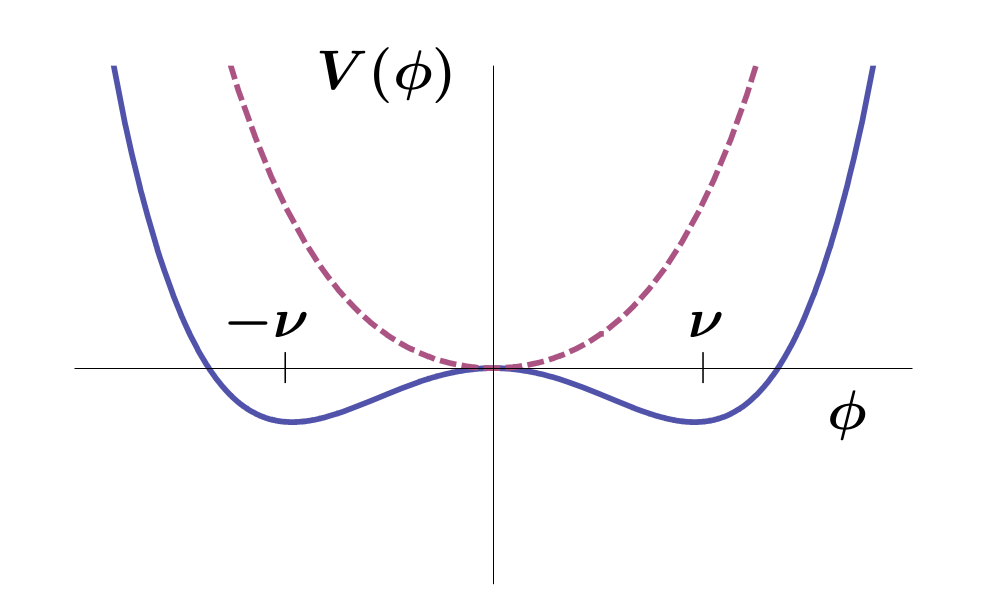
\includegraphics[scale=0.30]{./figures/potentiel_Higgs.png}
      \caption{ Potentiel de Higgs $V(\Phi)$ pour $\mu^2>0$ en ligne pointill\'ee violette et $\mu^2<0$ en ligne pleine bleue  }
      \label{fig:feynmanHiggs}
    \end{center}
  \end{figure} 
  
  Toujours pour $\mu^2<0$, on remplace le doublet de Higgs par sa valeur classique :
  
  \begin{equation}
   \Phi \rightarrow \dfrac{1}{\sqrt{2}} \begin{pmatrix} 0 \\ \nu \end{pmatrix} \equiv v
  \end{equation}

  Pour quantifier la th\'eorie autour du vide classique, on \'ecrit : $\Phi = v + \Phi'$. Dans le but d'identifier les particules physiques, on peut r\'e-\'ecrire les quatre composantes Hermitienne de $\Phi'$ en terme de nouvelles variables en utilisant la transformation de $Kibble$ \cite{Kibble:1967sv} :
  
  \begin{equation}
   \Phi = \dfrac{1}{\sqrt{2}} e^{i \sum_j \xi^jL^j} \begin{pmatrix} 0 \\ \nu + H \end{pmatrix}
  \end{equation}

  O\`u $H$ est un champ hermitien qui repr\'esentera le boson scalaire de Higgs. Si nous avions affaire \`a une brisure spontan\'ee globale de la sym\'etrie les trois champs Hermitiens $\xi^i$ seraient les bosons pseudo-scalaires sans masses de Nambu-Goldstone \cite{Nambu:1960xd, Nambu:1961tp, Goldstone:1961eq, Goldstone:1962es}. Cependant, dans une th\'eorie de jauge, ces trois degr\'es de libert\'e disparaissent pour donner les trois bosons massifs $W^\pm$ et $Z^0$. On peut le voir simplement en faisant la transformation de jauge suivante : 
  
  \begin{equation}
   \Phi \rightarrow \Phi' = e^{- i \sum_j \xi^j L^j} \Phi = \dfrac{1}{\sqrt{2}} \begin{pmatrix} 0 \\ \nu + H \end{pmatrix}
  \end{equation}
  
  Les bosons de Goldstone disparaissent. Avec cette jauge, le terme cin\'etique devient :

  \begin{equation}
   ( D_{\mu} \Phi )^\dagger D^{\mu} \Phi = \dfrac{1}{2} (0, \nu) \left[ \dfrac{g}{2} \tau^i W^i_{\mu} + \dfrac{g'}{2} B_{\mu} \right]^2 \begin{pmatrix} 0 \\ \nu \end{pmatrix} + \text{termes en H}
  \end{equation}

   
  O\`u les termes d'\'energie cin\'etique et de jauge en $H$ ne sont pas renseign\'es (termes en H). Il vient ensuite : 
  
  \begin{equation}
   ( D_{\mu} \Phi )^\dagger D^{\mu} \Phi = M_W^2 W^{+ \mu} W^-_{\mu} + \dfrac{M_Z^2}{2} Z^{\mu} Z_{\mu} + \text{termes en H}
  \end{equation}
  
  Avec : 
  
  \begin{equation}
   W^\pm = \dfrac{1}{\sqrt{2}} (W^1 \mp i W^2 )
  \end{equation}
  
  \begin{equation}
   Z = -\sin(\theta_W) B + \cos(\theta_W) W^3
  \end{equation}
  
  Le champ des photons vaut quant \`a lui :
  
  \begin{equation}
   A = \cos(\theta_W) B + \sin(\theta_W) W^3
  \end{equation}

  Ce qui revient au mixage suivant : 
  
  \begin{equation}
   \begin{pmatrix} A_{\mu} \\ Z_{\mu} \end{pmatrix} = \begin{pmatrix} \cos(\theta_W) & \sin(\theta_W) \\ -\sin(\theta_W) & \cos(\theta_W) \end{pmatrix} \begin{pmatrix} B_{\mu} \\ W_{\mu}^3 \end{pmatrix}
  \end{equation}

  O\`u $\theta_W$ est l'angle de Weinberg. 
  
  Les masses sont donn\'ees par : 
  
  \begin{equation}
   M_W = \dfrac{g \nu}{2}
  \label{eq:masseW}
  \end{equation}

  \begin{equation}
   M_Z = \sqrt{g^2+g'^2} \dfrac{\nu}{2} = \dfrac{M_W}{\cos(\theta_W)}
  \end{equation}

  \begin{equation}
   M_A = 0
  \end{equation}

  \begin{equation}
   M_H = \sqrt{-2\mu^2} = \sqrt{-2\lambda} \nu 
  \end{equation}

  L'angle de Weinberg s'exprime alors de la fa\c{c}on suivante : 
  
  \begin{equation}
   \theta_W = \arctan \left( \dfrac{g'}{g} \right) \quad \Rightarrow \quad \sin^2(\theta_W) = 1 - \dfrac{M_W^2}{M_Z^2}
  \end{equation}

  En utilisant la th\'eorie de Fermi, premi\`ere th\'eorie de l'interaction faible, on peut identifier le terme responsable de la d\'esint\'egration du muon et trouver son \'equivalent au plus bas ordre dans le mod\`ele standard. On obtient alors la relation suivante : 

  \begin{equation}
   \dfrac{G_F}{2} = \dfrac{g^2}{8 M_W^2}
  \end{equation}

  En utilisant l'équation \ref{eq:masseW} on obtient :
  
  \begin{equation}
   \dfrac{G_F}{\sqrt{2}} = \dfrac{1}{2 \nu^2} \Rightarrow \nu = \dfrac{1}{\sqrt{\sqrt{2} G_F}} \approx 246 \, GeV
  \end{equation}

  On identifie la charge du positon par : $e=g/\sin(\theta_W)$ avec $\theta_W \approx 0.23$. Ce qui donne pour les masses des bosons $W^\pm$ et $Z^0$ au premier ordre :
  
  \begin{equation}
   M_W \approx 78 GeV/c^2 \qquad M_Z \approx 89 \, GeV/c^2
  \end{equation}

  Ces masses sont augment\'ees de $2-3$ GeV apr\`es avoir rajout\'e la contribution des boucles. Les bosons W et Z ont \'et\'e d\'ecouverts au CERN en 1983 par les exp\'eriences UA1 \cite{Arnison:1985jk} et UA2 \cite{Ansari:1987vg}.
  Les masses mesur\'ees en 2013 selon le Particle Data Group sont :
  
  \begin{equation}
   M_W = 80.385 \pm 0.015 GeV/c^2 \qquad M_Z = 91.1876 \pm 0.0021 \, GeV/c^2
  \end{equation}

  Nous avons donc d\'ecrit brièvement le mod\`ele \'electrofaible et le m\'ecanisme de Higgs. Le LHC et les projets d'acc\'el\'erateurs de particules du futurs, comme l'ILC, permettront de d\'ecrire tr\`es finement cette physique. En particulier, l'\'etude des propri\'et\'es du boson Higgs seront mesur\'ees tr\`es pr\'ecis\'ement. Ces \'etudes confronteront le mod\`ele standard aux mesures exp\'erimentales tr\`es pr\'ecises. Des divergences avec le mod\`eles standard pourraient alors apparaître signant une nouvelle physique. Il faut ajouter \`a cela que malgr\'e son grand succ\`es, le mod\`ele standard ne d\'ecrit pas tous les ph\'enom\`enes physiques. C'est pourquoi, nous allons d\'ecrire les limitations du mod\`ele standard dans la prochaine section.
  
  \subsection{Limites du mod\`ele standard}
  
  Nous allons d\'ecrire dans cette section les limites du mod\`ele standard de la physique des particules. Nous d\'ecrirons tout d'abord les ph\'enom\`enes physiques, observ\'es, mais non inclus dans le mod\`ele standard, puis nous d\'ecrirons les limites th\'eoriques de ce mod\`ele.
  
  \subsubsection{Ph\'enom\`enes physiques non expliqu\'es par le mod\`ele standard}
  
  Le mod\`ele standard n'explique pas certaines observations physiques. Nous allons donner un aper\c{c}u de celles-ci. Premi\`erement le mod\`ele standard ne décrit pas la gravit\'e. M\^eme si aux \'echelles d'\'energie atteignables dans un collisionneur de particule actuel, la gravitation est n\'egligeable ($10^{-41}$ plus faible que la force forte), celle-ci devient non n\'egligeable \`a l'\'echelle de Planck ($10^{19}$ $GeV$). Diff\'erentes id\'ees permettant une th\'eorie quantique de la gravitation sont actuellement \`a l'\'etude. 
  
  \medskip
  
  Le mod\`ele standard n'explique pas non plus ni la mati\`ere noire ni l'\'energie sombre, or ces derni\`eres repr\'esentent respectivement environ 25\% et 70\% de la densit\'e d'\'energie de l'univers, pour seulement environ 5\% d\^u \`a la mati\`ere ordinaire. De plus dans le mod\`ele standard, les neutrinos ne poss\`edent pas de masse. Ces masses peuvent cependant \^etre rajout\'ees de mani\`ere \textit{ad hoc} au mod\`ele standard. 
  
  \medskip
  
  La question de la r\'epartition entre mati\`ere et anti-mati\`ere n'est pas non plus r\'esolue. Le mod\`ele standard pr\'edit que mati\`ere et anti-mati\`ere ont \'et\'e cr\'e\'ees en quantit\'es \'egales. Or les observations indiquent la pr\'esence d'une asym\'etrie mati\`ere-anti-mati\`ere. Les m\'ecanismes expliquant cette disproportion avec le mod\`ele standard, comme la violation de CP, ne sont pas suffisants pour expliquer le d\'ecalage observ\'e. De plus, la violation de CP a \'et\'e observ\'e dans le secteur \'electro-faible mais n'a pas \'et\'e mise en \'evidence pour les interactions fortes. 
  
  \medskip
  
  De surcro\^it, un autre probl\`eme est la hi\'erarchie des masses entre les fermions. Par exemple, le mod\`ele standard n'explique pas pourquoi la masse du quark top est cinq ordres de grandeur plus \'elev\'ee que la masse du quark up.
  
  \subsubsection{Limitations th\'eoriques}
  
  Certaines parties du mod\`ele standard, ont \'et\'e rajout\'ees de façon \textit{ad hoc} dans le but d'expliquer les ph\'enom\`enes physiques observ\'es. Ces rajouts, \`a l'instar du champ de Higgs, font partie int\'egrante du mod\`ele standard. Cependant, ils ne sont expliqu\'es par aucune n\'ecessité th\'eorique et augmentent le nombre de param\`etres libres non contraints th\'eoriquement du mod\`ele standard. Ces manquements th\'eoriques poussent \`a d\'evelopper des th\'eories plus fondamentales que le mod\`ele standard.
  
  \medskip
  
  Ainsi, le mod\`ele standard comporte des param\`etres libres, qui ne peuvent \^etre d\'etermin\'es qu'exp\'erimentalement. Historiquement ces param\`etres sont les neufs masses des fermions (9), les constantes de couplage des groupes $U(1)$ et $SU(2)$ $g$ et $g'$ et la constante de couplage de l'int\'eraction forte $\alpha_s$ (3), les 3 angles de m\'elange plus la phase de la matrice CKM (4), la masse du boson de Higgs et la valeur attendue du vide pour le champ de Higgs (vev) (2). S'ajoute encore, $\theta_{CP}^{QCD}$ (1), un param\`etre qui autorise la violation de CP dans le Lagrangien de QCD. Il s'agit l\`a des 19 param\`etres fondamentaux. On rajoutera que le param\`etre $\theta_{CP}^{QCD}$ a \'et\'e mesur\'e avec une valeur proche de z\'ero, ce qui pose le probl\`eme de la violation de CP forte. En effet, celle-ci n'a jamais \'et\'e observ\'ee alors que c'est le cas dans le domaine \'electrofaible. Pour obtenir des neutrinos massiques, on ajoute 7 nouvelles valeurs repr\'esentant les masses des 3 neutrinos (3) et les quatre param\`etres de la matrice de \textit{Pontecorvo-Maki-Nakagawa-Sakata} (équivalent de la matrice CKM pour les neutrinos massiques) (4). Nous en sommes \`a 26 param\`etres libres. Enfin, les observations cosmologiques tendent \`a indiquer que l'expansion de l'univers acc\'el\`ere. Une des explications est que le vide poss\`ede une densit\'e d'\'energie non nulle. Cette densit\'e d'\'energie, appel\'ee constante cosmologique $\Lambda$, (1), peut \^etre ajout\'ee comme extension au mod\`ele standard. Elle pourrait symboliser l'énergie sombre. Cela porte le nombre de param\`etres libres \`a au moins 27. 
  
  \medskip

  Par ailleurs, les valeurs des constantes de couplage $g$, $g'$ et $\alpha_s$, calcul\'ees \`a des \'energies \'elev\'ees (de l'ordre de $10^{15}$, $10^{16}$ $GeV$) ne convergent pas vers la m\^eme valeur, m\^eme si elles ont le m\^eme ordre de grandeur \`a ces \'echelles d'\'energies. La convergence de ces constantes est le signe d'une unification des forces \`a haute \'energie. Nous verrons plus loin que dans le cas de la supersymétrie ces constantes convergent pour une \'echelle d'\'energie de l'ordre de l'\'echelle de grande unification ($10^{16}$ $GeV$).

  \medskip
  
  Le probl\`eme de hiérarchie est aussi un probl\`eme majeur du mod\`ele standard, il concerne les particules scalaires. Nous expliquerons en quoi il consiste en prenant l'exemple du boson de Higgs. Soit $m_H$ la masse effective du boson de Higgs, $m_0$ sa masse nue et $\delta m_H$ ses corrections radiatives. On a :
  
  \begin{equation}
   m_H^2 = m_0^2 - \delta m_H^2
  \end{equation}

  Ainsi, lorsque l'on choisit une \'echelle d'\'energie $\Lambda$, repr\'esentant une coupure ultra-violette d\'efinissant la limite de validit\'e du mod\`ele standard ; que le Higgs se couple avec un fermion, un boson de jauge ou avec lui-m\^eme, les corrections radiatives obtenues sont quadratiques en $\Lambda$. On a ainsi :
  
  \begin{equation}
   \delta m_H^2 \propto \Lambda^2
  \end{equation}

  Prenons $\Lambda = \lambda_{GUT} = 10^{16}$ $GeV$ et $m_H \approx 100 \, GeV$. On a alors : 
  
  \begin{equation}
   m_H^2 \approx 10^4 \approx m_0^2 - 10^{32}
  \end{equation}

  Soit: 
  
  \begin{equation}
  10^{-28} \approx \cfrac{m_0^2}{10^{32}} - 1
  \end{equation}

  Ainsi, les 28 premi\`eres d\'ecimales du terme $\cfrac{m_0^2}{10^{32}}$ doivent \^etre ajust\'ees avec pr\'ecision. Il s'agit l\`a d'un ajustement extrêmement fin. Cet ajustement n'est pas "naturel" d'un point de vue th\'eorique. On parle de probl\`eme de naturalit\'e.  On notera que les corrections radiatives \`a la masse d'un fermion ont des divergences logarithmiques telles que : 
  
  \begin{equation}
   \delta m_f \propto m_f \ln \left(\cfrac{\Lambda^2}{m_f^2}\right)
  \end{equation}
  
  Ainsi m\^eme \`a l'\'echelle de grande unification $\Lambda_{GUT}$, $\delta m_f$ reste inf\'erieur \`a $m_f$
  
  \medskip
  
  Un autre probl\`eme th\'eorique est le probl\`eme de la violation de CP forte. Comme expos\'e plus haut, la violation de la sym\'etrie CP dans le domaine de la QCD n'a pas \'et\'e d\'emontr\'ee. Le coefficient $\theta^{QCD}_{CP}$ associ\'e au terme de violation de CP forte est proche de z\'ero.

  \medskip
  
  Afin de pallier \`a ces limitations, des th\'eories au delà du mod\`ele standard ont vu le jour. Nous allons r\'ealiser une revue non exhaustive des principales dans la suite de cette section.
  
  \subsection{Au delà du mod\`ele standard}
  
   Comme nous l'avons vu pr\'ec\'edemment, le mod\`ele standard connaît un grand succ\`es puisqu'il permet des pr\'edictions justes jusqu'au pour-mille. Cependant celui-ci poss\`ede des d\'efauts et certains processus physiques n'y sont pas pr\'esents. \`A l'heure actuelle, il s'av\`ere que selon toute vraisemblance le mod\`ele standard ne serait qu'une simplification \`a basse \'energie d'une th\'eorie plus compl\`ete. Dans le but de trouver une th\'eorie plus g\'en\'erale, qui pallierait aux d\'efauts du mod\`ele standard, plusieurs nouvelles th\'eories ont \'emerg\'e. Nous allons en d\'ecrire bri\`evement quelques unes.
   
   \medskip
   
   \subsubsection{GUT}
   
   Les th\'eories dites de grande unification (GUT) sont bas\'ees sur l'id\'ee suivante. Le mod\`ele standard d\'ecrit trois interactions fondamentales grâce au groupe de sym\'etrie $SU_C(3) \otimes SU_L(2) \otimes U_Y(1)$. Selon le mod\`ele standard, \`a des \'energies de l'ordre de $10^{16}$ GeV, appel\'ee \'energie de grande unification, les trois constantes de couplage se rapprochent d'une valeur commune, sans toutefois se rejoindre (voir figure \ref{fig:constCouplages}). Au dessus de cette \'energie, l'id\'ee est d'unifier ces trois interactions en une seule grâce \`a l'utilisation d'un groupe de sym\'etrie plus large poss\'edant une seule constante de couplage. En dessous de cette \'energie, la sym\'etrie est spontan\'ement bris\'ee et l'on retrouve le mod\`ele standard. Par exemple, les groupes de sym\'etries $SU(5)$ \`a cinq dimensions (mod\`ele de Georgi–Glashow), le groupe $SO(10)$ \`a dix dimensions et le groupe E6 ont \'et\'e \'etudi\'es. Les nouvelles particules pr\'edites par ces mod\`eles ont des masses de l'ordre de l'\'echelle de grande unification. Elles ne sont donc pas accessibles exp\'erimentalement. Cependant, les mod\`eles de grande unification souffrent de plusieurs limitations. Par exemple, la dur\'ee de vie du proton pr\'edite est tr\`es inf\'erieure \`a la valeur exp\'erimentale. 
   
   
%    Ces mod\`eles ont aussi des difficult\'es \`a reproduire les masses des fermions et la valeur de l'angle de Weinberg. D'autres ingr\'edients, comme la supersym\'etrie vont permettre d'obtenir des mod\`eles en accord avec les donn\'ees exp\'erimentales de pr\'ecision.

  \subsubsection{Supersym\'etrie}
  
  La \textit{supersym\'etrie} abr\'eg\'ee \textit{SUSY} est la th\'eorie au delà du mod\`ele standard la plus attrayante. Comme nous allons le voir, elle permet de s'affranchir de plusieurs limitations du mod\`ele standard. Cette th\'eorie associe \`a chaque particule un super-partenaire dont seul le spin diff\`ere de $\pm 1/2$. Autrement dit, \`a chaque fermion correspond un nouveau boson, et \`a chaque boson correspond un nouveau fermion. Les autres nombres quantiques des super-partenaires restant inchang\'es. Les super-partenaires cr\'e\'es par la th\'eorie sont appel\'es super-particules ou \textit{sparticules}. Les nouvelles sparticules sont appel\'ees de la façon suivante :
 
  \medskip
 
  \renewcommand{\labelitemi}{$\bullet$}
  \begin{itemize}
   \item les super-partenaires scalaires (spin 0) des champs de mati\`ere (fermions) prennent le nom de leur fermion correspondant dot\'e du suffixe \textit{s-} pour scalaire. Par exemple le super-partenaire de l'\'electron est nomm\'e s\'electron, celui d'un quark top, stop. 
   \item {les super-partenaires fermioniques des champs d'interaction (jauge et Higgs) portent le nom du boson correspondant suivi du suffixe \textit{-ino}. Ainsi, le jaugino associ\'e \`a un boson de Higgs, est nomm\'e Higgsino, celui d'un photon, photino.}
   \item Enfin, afin de diff\'erencier les abr\'eviations des particules du mod\`ele standard des super-partenaires, un tilde est ajout\'e au dessus. Ainsi, le super-partenaire de l'\'electron $e^-$, le s\'electron, est abr\'eg\'e $\widetilde{e^-}$
  \end{itemize}

  \medskip
  
  Les sparticules contribuent aux corrections radiatives \`a la masse du boson de Higgs \`a l'ordre de la boucle, et en utilisant certaines hypoth\`eses (comme $\lambda_f^2 = -\lambda_{\widetilde{s}}$), le terme de divergence quadratique avec l'\'echelle d'énergie $\Lambda$ est annul\'e. Le probl\`eme de hiérarchie est alors r\'esolu. Seul reste une divergence logarithmique. Si la supersym\'etrie \'etait une sym\'etrie exacte, les masses des couples particules-sparticules seraient les m\^emes. Par exemple \'electrons et s\'electrons auraient la même masse de 511 $keV/c^2$. Cependant \`a ce jour, aucune sparticule n'a \'et\'e d\'etect\'ee. Cela implique que la supersymétrie est une sym\'etrie bris\'ee. Une masse plus \'elev\'ee pour les sparticules est alors permise. La brisure de la \textit{SUSY} doit se faire de façon \`a ne pas faire r\'eappara\^itre des corrections radiatives pr\'esentant des divergences quadratiques. Pour cela la diff\'erence entre les masses des particules et des sparticules correspondantes ne doit pas \^etre trop grande. Une SUSY bris\'ee en dessous de l'ordre du $TeV$ permet de s'affranchir du probl\`eme de l'ajustement fin des param\`etres. 
  \medskip
  
  Diff\'erents mod\`eles de particules supersym\'etriques appliqu\'es au mod\`ele standard existent. La diff\'erence entre ces mod\`eles est le contenu en champs. Le \textit{MSSM} ou mod\`ele supersymétrie du mod\`ele standard est l'extension minimale supersymétrique du modèle standard ; elle a un contenu en champ minimal mais requiert un deuxième doublet de champs scalaires de Higgs pour briser spontanément la symétrie électrofaible. \`A ces deux doublets de Higgs sont associ\'es deux doublets de Higgsinos. La pr\'esence d'un second doublet pour le secteur de Higgs assure une masse \`a toutes les super-particules et permet d'\'eviter les anomalies triangulaires qui ne permettent pas de conserver la sym\'etrie de jauge locale associ\'ee au champ $A_{\mu}$.
  
  
  \medskip
  
  On rappelle que dans le mod\`ele standard, il n'existe qu'un seul doublet de Higgs, scalaire complexe, donnant lieux \`a quatre degr\'es de libert\'e. Trois d'entre eux deviennent des bosons de Goldstone ($G^0,G^{\pm}$) sans masse. Ces bosons sont ensuite "absorb\'es" lors de la brisure de sym\'etrie \'electrofaible par les bosons de jauge $Z^0$ et $W^{\pm}$ qui deviennent alors massifs. Le degr\'e de libert\'e restant dans le mod\`ele standard est associ\'e au boson de Higgs standard. La pr\'esence d'un second doublet de Higgs implique l'existence de quatre nouveaux degr\'es de libert\'e. On obtient donc $4 + 1 = 5$ particules au total. Cela conduit \`a la pr\'ediction de cinq bosons de Higgs. Deux bosons de Higgs neutres  $h^0$ et $H^0$ et paires sous CP, un boson de Higgs neutre $A^0$ et impaire sous CP, et enfin deux bosons de Higgs charg\'es $H^+$ et $H^-$. Le boson de Higgs le plus l\'eger \'etant le boson $h^0$. Il s'agit peut-être de celui d\'ecouvert au LHC. La valeur $\tan(\beta) = v_1/v_2$ repr\'esente le rapport des deux valeurs attendues dans le vide de deux doublets de Higgs. Nous en reparlerons plus loin lors de la description de la physique \`a l'ILC.

  \begin{figure}[!htb]
    \begin{center} 
      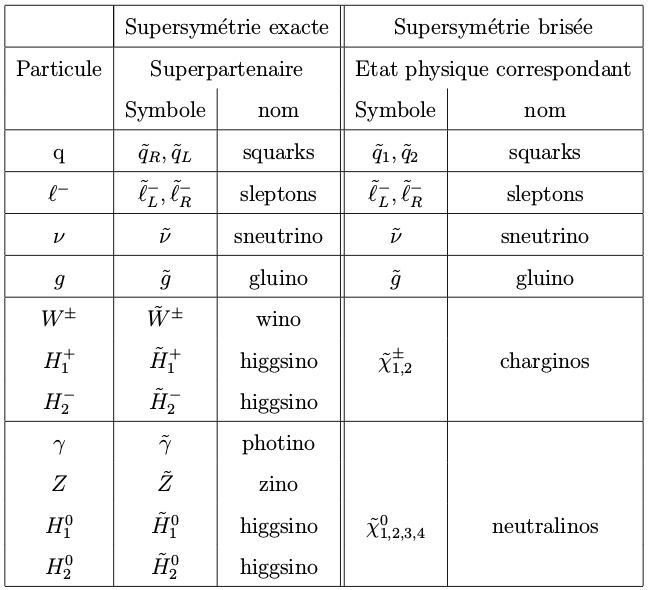
\includegraphics[scale=0.50]{./figures/tableau_SUSY.png}
      \caption{Liste des particules et super-partenaires du \textit{MSSM}, avec les noms des champs des super-partenaires et de l'\'etat physique correspondant apr\`es brisure de la supersymétrie.}
     \label{fig:etatsPropresMasse}
     \end{center}
  \end{figure} 
  
  \medskip
  
  Lorsque la supersym\'etrie est spontan\'ement bris\'ee, les jauginos neutres, poss\'edant les m\^emes nombres quantiques, se m\'elangent pour donner des \'etats propres de masse. Le m\'elange des higgsinos, bino et wino conduit \`a quatre particules appel\'ees neutralinos. On les note $\widetilde{\chi}_{1,2,3,4}$. Le neutralino $\widetilde{\chi}_{1}$ \'etant le plus l\'eger et le neutralino $\widetilde{\chi}_{4}$ le plus lourd. Selon le m\^eme principe les bosons charg\'es $H^{\pm}$ et $W^{\pm}$ se m\'elangent pour donner deux \'etats de masses appel\'ees charginos $\widetilde{\chi}^{\pm}_{1,2}$. Pour les sfermions, les \'etats propres de masse sont des superpositions des \'etats propres de jauge des sfermions. On notera que les sfermions sont les super-partenaires des fermions droits et gauches. Comme les sfermions sont de spin 0, ils ne sont ni droits ni gauches. Cependant, on leur adjoint un indice $R$ ou $L$ pour rappeler de quels fermions ils sont issus. Les \'etats propres de masse physique sont donn\'es en figure \ref{fig:etatsPropresMasse}.
  
  \medskip
  
  \begin{figure}[!htb]
    \begin{center} 
      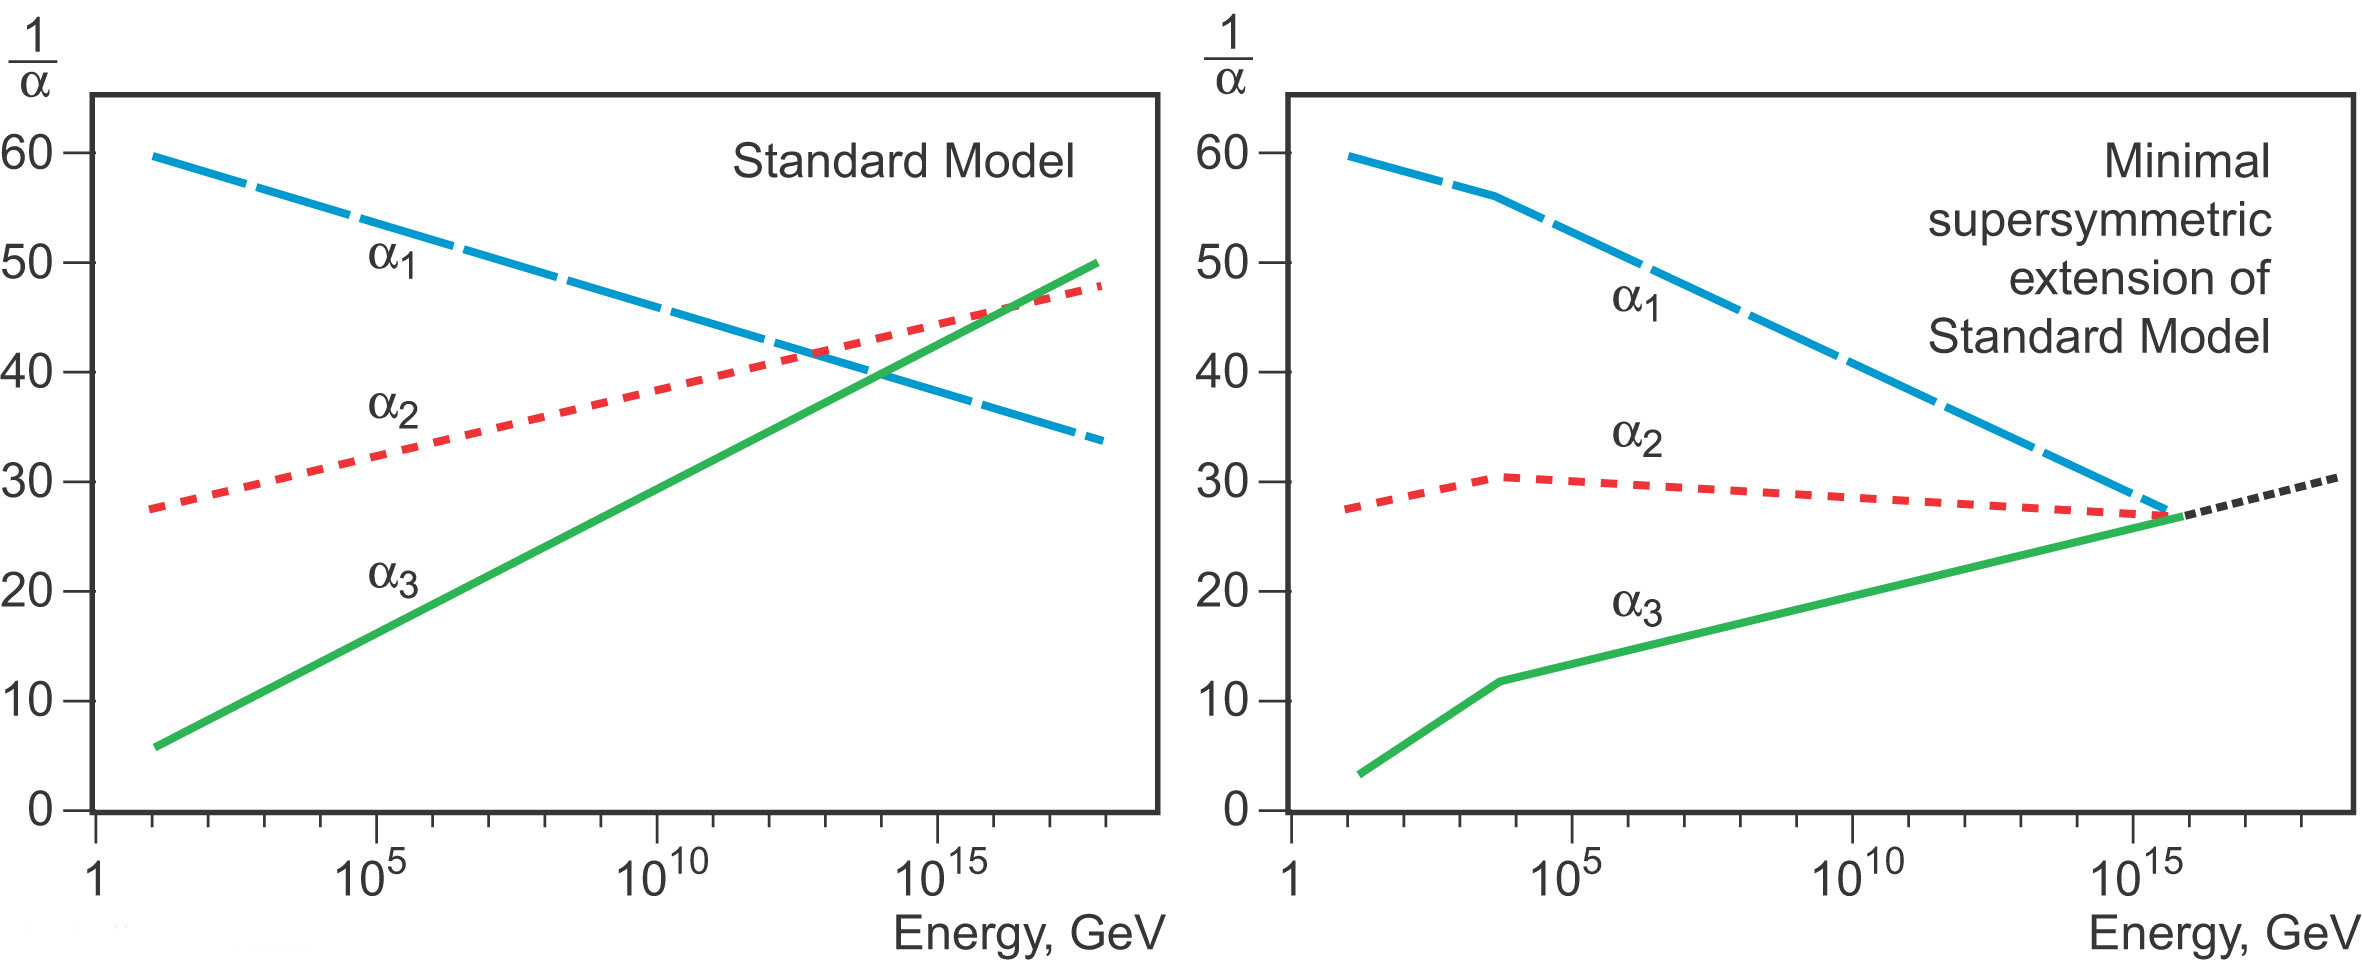
\includegraphics[scale=0.70]{./figures/constantes_couplage_MS_SUSY.jpg}
      \caption{\'Evolution des constantes de couplage pour le mod\`ele standard, à droite, et pour le mod\`ele supersym\'etrique minimal \`a droite. Dans le cas de la supersym\'etrie, les trois constantes se rejoignent \`a l'\'energie de grande unification de $10^{16}$ GeV. }
     \label{fig:constCouplages}
     \end{center}
  \end{figure}
  
  La supersymétrie permet aussi l'unification des constantes de couplage des trois forces fondamentales d\'ecrites \`a l'\'echelle de grande unification (voir figure \ref{fig:constCouplages}). De plus, la supersymétrie n'implique pas la conservation du nombre baryonique B et du nombre leptonique L. La violation de ces nombres implique entre autre la d\'esint\'egration rapide du proton. Une nouvelle sym\'etrie a donc \'et\'e ajout\'ee : la R-Parit\'e. La R-Parit\'e est d\'efinie par : 
  
  \begin{equation}
   R_p = (-1)^{3B+2S+L}
  \end{equation}

  Avec $B$ le nombre baryonique, $L$ le nombre leptonique et $S$ le spin. Les super-partenaires poss\`edent une R-parit\'e n\'egative alors que les particules du mod\`ele standard poss\`edent une R-parit\'e positive. Cela entraîne de nombreuses propri\'et\'es ph\'enom\'enologiques. 
  
  \medskip
  
  \renewcommand{\labelitemi}{$\bullet$}
  \begin{itemize}
   \item les sparticules ne peuvent \^etre produites que par paire,
   \item la sparticule la plus l\'eg\`ere est n\'ecessairement stable puisqu'elle ne peut se d\'esint\'egrer en une autre sparticule plus l\'eg\`ere,
    \item les sparticules autres que la plus l\'eg\`ere, se d\'esint\`egrent en une ou deux particules du mod\`ele standard et une seule sparticule.
  \end{itemize}

  \medskip
  
%   La particule supersym\'etrique la plus l\'eg\`ere est un bon candidat de particule n'interagissant que très faiblement (\textit{WIMPS}) et pourrait contribuer \`a la grande masse de la mati\`ere noire d\'eduite des mesures cosmologiques. 
  
  Dans le \textit{MSSM} les neutralinos, sparticules neutres, sont des particules apparaissant apr\`es la brisure de la supersymétrie, ils sont un mixage entre jauginos \'electrofaibles et Higgsinos. Le neutralino le plus l\'eger, correspondant \`a la particule supersym\'etrique la plus l\'eg\`ere, serait un bon candidat pour expliquer la mati\`ere noire. 
  
  \medskip
  
  Certains mod\`eles supersym\'etriques \`a R-parit\'e viol\'ee conservent une dur\'ee de vie du proton acceptable, mais postulent une particule supersymétrique la plus l\'eg\`ere non stable. Toutefois, ces mod\`eles engendrent une ph\'enom\`enologie diff\'erentes, puisque les r\`egles d\'efinies ci-dessus ne sont plus valables.
  
  \medskip
  
  A l'heure de l'écriture de ce chapitre, le LHC \`a 7 et 8 $TeV$ n'a r\'ev\'el\'e aucun signe de supersymétrie. La possibilit\'e de d\'ecouverte de particules supersym\'etriques sous le $TeV$ a fortement \'et\'e restreinte. Le programme \`a 13/14 $TeV$ du LHC devrait débuter début 2015 et devrait fournir de nouvelles d\'ecouvertes ou exclusions.
  
  \subsubsection{Autres mod\`eles au del\`a du mod\`ele standard}
  
  Parmi les autres th\'eories au-delà du mod\`ele santadard se trouve les th\'eories des cordes et super-cordes, les dimensions suppl\'ementaires, la compositness, la technicouleur, les th\'eories de la gravitation modifi\'ee (MoND), la gravitation quantique \`a boucle ; et bien d'autres. Nous ne reviendrons pas en d\'etail sur ces th\'eories.
  
%   Appliqu ́ee aux particules du Mod`ele Standard, la supersym ́etrie donne naissance `a une
% classe de mod`eles dont la diff ́erence principale est le contenu en champs.
% Nous allons nous attacher `a un mod`ele en particulier, le Mod`ele Standard Super-
% sym ́etrique Minimal (MSSM) qui reprend juste le contenu en champs du MS ainsi que
% leurs superpartenaires. 
%   
% 
%  
%  Pour donner de la masse `a tous les superchamps mat ́eriels, mais  ́egalement pour annu-
% ler les divergences dues aux diagrammes triangulaires contenant un higgsino interne  il a fallu faire appel `a un doublet suppl ́ementaire de Higgs.
% 
% 
% Ces diagrammes se compensent exactement dans le cadre du Mod`ele Standard en
% sommant sur toutes les esp`eces fermioniques. Pour maintenir cette compensation dans le
% cadre du MSSM,il faut deux higgsinos d’hypercharge Y oppos ́ees.
%   
% %   Among the most popular is Supersymmetry (SUSY) [Singer ℄, whi
% h is the only
% % renormalisable Quantum Field Theory (QFT) among all alternatives of the SM 
% onsid-
% % ered up to now. SUSY is an additional symmetry that relates ea
% h known elementary
% % fermion with a 
% orresponding boson, and vi
% e versa. The two related parti
% les are
% % 
% alled superpartners. They are a priori expe
% ted to have exa
% tly the same mass and
% % quantum numbers, ex
% ept that their spin will dier by 1/2. Su
% h a symmetry has not
% % yet been found in Nature. There is no experimental eviden
% e of any SUSY relating
% % known elementary fermions and bosons. So, if supersymmetry exists, it will be a broken
% % symmetry. This will allow the supersymmetri
%  parti
% le to a
% quire very high masses,
% % explaining this way why they were not experimentally observed until now.
% % SUSY extension of the SM addresses a variety of the 
% urrently open issues of parti
% le
% % physi
% s. It provides a natural solution to the hierar
% hy problem. The loop 
% ontributions
% % on the higgs mass arising from the bosoni
%  and fermioni
%  superpartners will be mutually
% % 
% an
% elled. Thus the hierar
% hy problem will be solved without the ne
% essity to perform
% % any ne tuning. The SUSY also allows for the uni
% ation of the three gauge intera
% tions
% % at a 
% ommon GUT s
% ale. Moreover, the lightest supersymmetri
%  parti
% le, will be a
% % promising 
% andidate for (at least a part of) the dark matter. Therefore, if SUSY
% % manifestations are found, numerous fundamental questions should be answered. But a
% % new one will also arise: why is SUSY broken?
% % A large fra
% tion of the allowed parameter spa
% e of SUSY has been ex
% luded by the
% % LEP and Tevatron experiments. Within the LHC perspe
% tives, it is expe
% ted that the
% % SUSY energy s
% ale is typi
% ally around 1 TeV. If this s
% ale will be found to be well above
% % 1 TeV would a
% tually 
% ontradi
% t the benet of SUSY for 
% ontrolling mass divergen
% es.
% % Thus if it exists, supersymmetri
%  parti
% les should be dis
% overed at the LHC.
  
%    
%    The term Grand Unified Theory or GUT, refers to any of several similar models in particle physics in which at high energy scales, the three gauge interactions of the Standard Model which define the electromagnetic, weak, and strong interactions, are merged into one single interaction characterized by a larger gauge symmetry and one unified coupling constant rather than three independent ones. The physics of most models of grand unification cannot be discovered directly at particle colliders because the new particles they predict have masses at the so-called GUT scale which lies few orders of magnitude below the Planck scale and thus far beyond the reach of collision experiments. Instead, information about grand unification might be obtained through indirect observations such as proton decay or the properties of neutrinos. [1] Some grand unified theories predict the existence of magnetic monopoles.
% 
% Currently (2011), all GUT models which aim to be completely realistic are quite complicated even compared to the Standard Model because they need to introduce additional structures such as new fields and interactions, or even additional dimensions of space. The main reason for this lies in the difficulty of reproducing the observed fermion masses and mixing. Due to these problems and the apparent impossibility to observe the physics of grand unification directly in experiments, there is no generally accepted GUT model.
%    
%    La supersym\'etrie, abr\'eg\'ee SuSy est une des th\'eorie des plus int\'eressante permettant d'\'etendre le mod\`ele standard.
%   
%   Because their masses are predicted to be just a few orders of magnitude below the Planck scale, at the GUT scale, well beyond the reach of foreseen particle colliders experiments, novel particles predicted by GUT models cannot be observed directly. Instead, effects of grand unification might be detected through indirect observations such as proton decay, electric dipole moments of elementary particles, or the properties of neutrinos.[1] Some grand unified theories predict the existence of magnetic monopoles.
% 
% As of 2012, all GUT models which aim to be completely realistic are quite complicated, even compared to the Standard Model, because they need to introduce additional fields and interactions, or even additional dimensions of space. The main reason for this complexity lies in the difficulty of reproducing the observed fermion masses and mixing angles. Due to this difficulty, and due to the lack of any observed effect of grand unification so far, there is no generally accepted GUT model.
%   
%   Grand unified theories[edit]
% Main article: Grand Unified Theory
% The standard model has three gauge symmetries; the colour SU(3), the weak isospin SU(2), and the hypercharge U(1) symmetry, corresponding to the three fundamental forces. Due to renormalization the coupling constants of each of these symmetries vary with the energy at which they are measured. Around 1016 GeV these couplings become approximately equal. This has led to speculation that above this energy the three gauge symmetries of the standard model are unified in one single gauge symmetry with a simple group gauge group, and just one coupling constant. Below this energy the symmetry is spontaneously broken to the standard model symmetries.[9] Popular choices for the unifying group are the special unitary group in five dimensions SU(5) and the special orthogonal group in ten dimensions SO(10).[10]
% 
% Theories that unify the standard model symmetries in this way are called Grand Unified Theories (or GUTs), and the energy scale at which the unified symmetry is broken is called the GUT scale. Generically, grand unified theories predict the creation of magnetic monopoles in the early universe,[11] and instability of the proton.[12] Neither of which have been observed, and this absence of observation puts limits on the possible GUTs.
% 
% Supersymmetry[edit]
% Main article: Supersymmetry
% Supersymmetry extends the Standard Model by adding an additional class of symmetries to the Lagrangian. These symmetries exchange fermionic particles with bosonic ones. Such a symmetry predicts the existence of supersymmetric particles, abbreviated as sparticles, which include the sleptons, squarks, neutralinos and charginos. Each particle in the Standard Model would have a superpartner whose spin differs by 1/2 from the ordinary particle. Due to the breaking of supersymmetry, the sparticles are much heavier than their ordinary counterparts; they are so heavy that existing particle colliders may not be powerful enough to produce them.
% 
% Neutrinos[edit]
% In the standard model, neutrinos have exactly zero mass. This is a consequence of the standard model containing only left-handed neutrinos. With no suitable right-handed partner, it is impossible to add a renormalizible mass term to the standard model.[13] Measurements however indicated that neutrinos spontaneously change flavour, which implies that neutrinos have a mass. These measurements only give the relative masses of the different flavours. The best constraint on the absolute mass of the neutrinos comes from precision measurements of tritium decay, providing an upper limit 2 eV, which makes them at least five orders of magnitude lighter than the other particles in the standard model.[14] This necessitates an extension of the standard model, which not only needs to explain how neutrinos get their mass, but also why the mass is so small.[15]
% 
% One approach to add masses to the neutrinos, the so-called seesaw mechanism, is to add right-handed neutrinos and have these couple to left-handed neutrinos with a Dirac mass term. The right-handed neutrinos have to be sterile, meaning that they do not participate in any of the standard model interactions. Because they have no charges, the right-handed neutrinos can act as their own anti-particles, and have a Majorana mass term. Like the other Dirac masses in the standard model, the neutrino Dirac mass is expected to be generated through the Higgs mechanism, and is therefore unpredictable. The standard model fermion masses differ by many orders of magnitude; the Dirac neutrino mass has at least the same uncertainty. On the other hand, the Majorana mass for the right-handed neutrinos does not arise from the Higgs mechanism, and is therefore expected to be tied to some energy scale of new physics beyond the standard model, for example the Planck scale.[16] Therefore, any process involving right-handed neutrinos will be suppressed at low energies. The correction due to these suppressed processes effectively gives the left-handed neutrinos a mass that is inversely proportional to the right-handed Majorana mass, a mechanism known as the see-saw.[17] The presence of heavy right-handed neutrinos thereby explains both the small mass of the left-handed neutrinos and the absence of the right-handed neutrinos in observations. However, due to the uncertainty in the Dirac neutrino masses, the right-handed neutrino masses can lie anywhere. For example, they could be as light as keV and be dark matter,[18] they can have a mass in the LHC energy range[19][20] and lead to observable lepton number violation,[21] or they can be near the GUT scale, linking the right-handed neutrinos to the possibility of a grand unified theory.[22][23]
% 
% The mass terms mix neutrinos of different generations. This mixing is parameterized by the PMNS matrix, which is the neutrino analogue of the CKM quark mixing matrix. Unlike the quark mixing, which is almost minimal, the mixing of the neutrinos appears to be almost maximal. This has led to various speculations of symmetries between the various generations that could explain the mixing patterns.[24] The mixing matrix could also contain several complex phases that break CP invariance, although there has been no experimental probe of these. These phases could potentially create a surplus of leptons over anti-leptons in the early universe, a process known as leptogenesis. This asymmetry could then at a later stage be converted in an excess of baryons over anti-baryons, and explain the matter-antimatter asymmetry in the universe.[10]
% 
% The light neutrinos are disfavored as an explanation for the observation of dark matter, due to considerations of large-scale structure formation in the early universe. Simulations of structure formation show that they are too hot—i.e. their kinetic energy is large compared to their mass—while formation of structures similar to the galaxies in our universe requires cold dark matter. The simulations show that neutrinos can at best explain a few percent of the missing dark matter. The heavy sterile right-handed neutrinos are however a possible candidate for a dark matter WIMP.[25]
%   
%   
%   Malgr\'e la tres bonne concordance entre les r\'esultats exp\'erimentaux et le mod\`ele standard, quelques questions reste en suspend. Nous allons ici les exposer.
%   
%   
%   
%   Nombre de param\`etre libres.
%   Mati\`ere noire
%   Mati\`ere/Antimati\`ere
%   Probl\`eme de hierarchie.
%   violation de CP
%   Gravitation et Relativit\'e G\'en\'erale.
%   GUT scales.
%     
%    La supersym\'etrie.
%    \medskip
%    Compositeness
%    \medskip
%    Th\'eorie des cordes Supercordes th\'eorie M.
%    \medskip
%    ExtraDim
%    \medskip
%    Th\'eorie quantiques de la gravitation.
%    \medskip
%    D'autre th\'eories physiques sont en \'elaboration afin de d\'epasser le mod\`ele standard. Parmi celle-ci se trouve les GUT, la supersym\'etrie, la th\'eorie des corde ou encore ...  Extra. Dim.
  
%   \section{Dispositifs exp\'erimentaux : les diff\'erents types de colisionneurs de particules}
%   
%   les dispositifs exp\'erimentaux pour la physique des particules : les collisionneurs et l'astrophysique.
%   
%   \subsection{Introduction}
%   Ce qui a d\'ej\`a \'et\'e d\'ecouvert avec les ancien et actuels colisionneurs. \\
%   Nouvelle d\'ecouverte : le boson de Higgs. \\
%   
%   \subsection{Le boson de Higgs : d\'ecouverte et questionnement}
%   
%   Higgs du mod\`ele standard ? \\
%   "Usine" \`a Higgs nécessaire \\
%   
%   \subsection{Les collisionneurs du futur}
%   
%   Explorer le domaine d'energie 100GeV -> TeV voir jusqu'a 100 TeV.
%   
%   \subsubsection{Collisionneurs leptoniques ou hadroniques}
%   
%   Avantages et inconv\'enients. \\
%   Limitations technologiques et pratiques \\
%   Ce qui peut se faire dans un futur proche. \\
%   
%   \subsubsection{Colisionneurs lin\'eaires}
%   
%   $e^+$ $e^-$ : ILC,CLIC
%   
%   \subsubsection{Les futur collisionneurs circulaires}
%   
%   (FCC) \\
%   Collisionneurs Hadroniques : HL-LHC, FHC, VLHC. \\
%   Collisionneurs Leptoniques : LEP3,FEC,$\mu \mu C$. \\
%   Collisionneurs "hybride" : LHeC. \\
%   
%   \subsubsection{L'ILC}
%   
%   Int\'er\^et de l'ILC : Principales caract\'eristiques et physique possible. \\
%   
%   \section{ILC}
%   
%   Intro \\
%   
%   \subsection{Programme de physique}
%   
%   En fonction de l'\'energie dans le centre de masse. \\
%   Higgs diff\'erents Couplages, BR \\
%   Physique du Top \\
%   Autres \\
%   
%   \subsection{Bruit de fond}
%   
%   Beanstrahlung \\
%   Taux d'occupation \\
%   
%   \subsection{D\'etecteurs}
%   
%   Historiquement 2 d\'etecteurs. Mais maintenant : Un ou peut-\^etre deux ? ... \\
%   ILD et SID : 2 voies diff\'erentes \\
%   
%   \subsubsection{ILD}
%   
%   D\'etecteur de Vertex \\
%   Trajectom\`etre \\
%   Colorim\`etres \\
%   Champs magn\'etique et culasse (+ muons) \\
%   
%   \chapter{D\'etecteur de vertex}
%   
%   Intro et motivations \\
%   
%   \section{Comparaison des technologies existantes}
%   
%   Pixels Hybrides \\
%   DEPFET \\
%   Fine Pixel CDD \\
%   CMOS \\
%   
%   \section{Capteurs CMOS pour le d\'etecteurs de vertex de l'ILD}
%   
%   CMOS -> LA bonne technologie pour les d\'etecteurs de vertex du futur.
%   
%   \subsection{Contraintes sur l'identification des saveurs et performances requises}
%   
%   Identification et distinction des vertex d\'eplac\'es -->  Contrainte sur le param\`etre d'impact. \\
%   Taux d'occupation, bruit de fond faisceau et tol\'erance au radiations \\
%   
%   \subsection{Capteurs CMOS : fonctionnement et performances}
%   
%   Fonctionnement \\
%   Points forts et performances \\
%   Etat de l'art : MIMOSA 28 \\
%   
%   \subsection{D\'etecteur de vertex de l'ILD compos\'e de capteurs CMOS}
%   
%   Les diff\'erents capteurs et \'echelles possibles. \\
%   Vitesse vs R\'esolution vs consommation \\
%   Échelles doubles faces  => Mini-vecteurs => Nouvelles perspectives sur l'alignement et la trajectom\'etrie ? \\
%   
%   \subsection{T\'elescope en faisceau AIDA et d\'eveloppement des techniques}
%   
%   Permet diff\'erentes \'etudes dans le cadre du d\'eveloppement des capteurs et \'echelles pour les futur d\'etecteurs de vertex. \\
%   Permet le d\'eveloppement des techniques d'alignement et de trajectom\'etrie de demain. \\
%   transition chapitre tests en faisceau. \\
  
  
  \section{Dispositifs exp\'erimentaux : les diff\'erents types de colisionneurs de particules}
  
  Afin de progresser en physique des particules, des dispositifs exp\'erimentaux sont requis. Motiv\'es par la d\'ecouverte de nouveaux ph\'enom\`enes physiques, les acc\'el\'erateurs de particules ne cessent de voir leur \'energie et/o\`u leur luminosit\'e augmenter. En passant de la centaine de $keV$ pendant les ann\'ees 30 \`a la dizaine de $TeV$ de nos jours avec le LHC, les sauts en énergies des acc\'el\'erateurs ont permis des avanc\'ees  majeures en physiques des particules. On peut citer parmi les principaux acc\'el\'erateurs de particules de la derni\`ere d\'ecennie : le \textit{Tevatron}, \textit{Super KEKB} et derni\`erement le LHC. Dans cette section nous d\'ecrirons les principaux types d'acc\'el\'erateurs puis nous exposerons les derni\`eres principales d\'ecouvertes en physique des hautes \'energies depuis les ann\'ees 1995. Enfin, nous d\'ecrirons les nouveaux projets d'acc\'el\'erateurs qui pourront voir le jour dans les d\'ecennies \`a venir et leurs motivations.

%   \subsection{Physique des accélérateurs}
% 
%   Voyons pourquoi les acc\'el\'erateurs de particules sont n\'ecessaires pour comprendre les lois physiques de l'univers. La relation de Louis De Broglie, postulant la dualité onde-corpuscule, permet de comprendre intuitivement pourquoi les accélérateurs de particules sont des outils primordiaux pour sonder la physique des particules élémentaires. Cette relation s'écrit :
%   
%   \begin{equation}
%    \lambda = \cfrac{h}{p} = \cfrac{h}{mv} \sqrt{1-\cfrac{v^2}{c^2}}
%   \end{equation}
% 
%   Avec $\lambda$ la longueur d'onde associ\'ee \`a la particule, $h$ la constante de Planck et $p$ la quantit\'e de mouvement de la particule. Appliquons cette relation dans le cas d'un faisceau de particule. La vitesse relativiste $v$ d'une particule de masse $m_0$ et d'énergie cin\'etique $E_c$ dans un acc\'el\'erateur est donn\'ee par :
%   
%   \begin{equation}
%    \cfrac{v}{c} = \sqrt{1- \left( \cfrac{1}{1+\cfrac{E_c}{m_0 c^2}} \right)^2}
%   \end{equation}
% 
%   Pour un acc\'el\'erateur $e^+$ $e^-$ dot\'e d'une \'energie dans le centre de masse de l'ordre du $TeV$, on obtient : $\lambda \approx 5 \, 10^{-19} \, m$ soit $5 \, 10^{-4} \, fm$. On peut donc sonder des objets physiques de cet ordre de grandeur, extrêmement petit. Même si la notion de taille n'est pas rigoureuse en m\'ecanique quantique, cette relation permet de montrer que l'on peut sonder la mati\`ere \`a des niveaux extr\^emement fins. On peut aussi rappeler la longueur de \textit{Planck} valant environ $10^{-35} \, m$.
  
%   \subsubsection{Section efficaces et luminosit\'e}
%   
%   Les r\'eactions $e^+$ $e^-$ permettent diff\'erents \'etats finals. En physique des particules la probabilit\'e qu'un certain processus de d\'esint\'egration soit produit est reli\'ee \`a une valeur nomm\'ee section efficace. Cette grandeur est exprim\'ee en \textit{barn} et est très souvent not\'ee $\sigma$. Un \textit{barn} valant $10^{-24} cm^2$. Les valeurs des sections efficaces peuvent \^etre calcul\'ees plus ou moins pr\'ecis\'ement son la th\'eorie que l'on consid\`ere. L'ordre de grandeur des sections efficace en physique des particules varie entre le femtobarn et le barn. Ces ordres de grandeurs dépendant du type de collisions effectu\'ees dans le collisionneur.
%   
%   \medskip
%   
%   Ces sections efficaces \'etant tr\`es faibles, il faut alors produire une tr\`es grand nombre de collisions pour pouvoir observer les \'ev\'enements int\'eressants. Le nombre moyen d'\'ev\'enements d'un certain type cr\'e\'es par unit\'e de temps est donn\'e par la relation suivante :
%   
%   \begin{equation}
%    \cfrac{dN}{dt} = L \sigma
%   \end{equation}
% 
%   Avec $L$ une grandeur appel\'ee luminosit\'e et $\sigma$ la section efficace du processus consid\'er\'e. La luminosit\'e est exprim\'ee en $cm^{-2}s^{-1}$ ou encore en $b^{-1}s^{-1}$. Ainsi, la luminosit\'e repr\'esente une densit\'e d'\'ev\'enements par unit\'e de surface et de de temps. On notera que le nombre d'\'ev\'enements produit durant une certaine dur\'ee peut \^etre exprim\'es en $b^{-1}$. L'unit\'e souvent utilis\'ee est le $fb^{-1}$, elle correspond \`a $10^{15}$ \'ev\'enements enregistr\'es.
  
  \subsubsection{Cas du collisionneur}
  
  L'id\'ee du collisionneur de particules a permis de fortement augmenter l'\'energie dans le centre de masse, compar\'e, \`a un acc\'el\'erateur dot\'e d'un faisceau frappant une cible. Nous allons le montrer par un calcul simple.
  
  \medskip
  
  L'\'energie disponible dans le centre de masse, dans le cas d'un faisceau de proton de masse $m_0$ et d'\'energie cin\'etique $E$ projet\'e sur une cible vaut : 
 
  \begin{equation}
   E_{CM} = \sqrt{2 m_0 (E + m_0)}
  \end{equation}

  Par exemple pour des protons de 7 $TeV$, on a $E_{CM} = 118.3 \, GeV$. Dans le cas d'un collisionneur de deux particules identiques d'\'energie cin\'etique E on a :
  
  \begin{equation}
   E_{CM} = 2 E
  \end{equation}

   Pour des protons de 7 $TeV$ on a $E_{CM} = 14 \, TeV$. L'\'energie disponible dans le centre de masse est donc tr\`es sup\'erieure dans le cas d'un collisionneur.
    
  \subsubsection{Collisionneur circulaire}
  
  Une particule ultra-relativiste \'emet un rayonnement synchrotron lorsqu'elle parcourt une trajectoire courbe. La puissance dissip\'ee est donn\'ee par :

  \begin{equation}
   \Delta E \propto \cfrac{E^4}{m^4R}
  \end{equation}
  
  O\`u $E$ est l'\'energie de la particule, $m$ sa masse et $R$ le rayon de courbure. Calculons le rapport d'\'energie perdue entre un proton et un \'electron, tous deux pris dans le cas ultra-relativiste. On a :
  
  \begin{equation}
   \cfrac{\Delta E_e}{\Delta E_p} = \cfrac{m_p^4}{m_e^4} \approx 1836^4 \approx 1.1 \, 10^{13}
  \end{equation}

  L'\'energie synchrotron dissip\'ee, \`a rayon \'egal, est treize ordres de grandeur sup\'erieure pour un \'electron compar\'e \`a un proton. La mont\'ee en \'energie est donc plus facile pour un faisceau de proton que pour un faisceau d'\'electron. Cette relation implique aussi qu'\`a m\^eme \'energie, il faut un anneau d'acc\'el\'eration plus grand pour les \'electrons que pour les protons. \`A l'heure actuelle, le LEP avec son anneau de 27 km de circonf\'erence a \'etabli le record d'\'energie dans le centre de masse pour un collisionneur $e^+$ $e^-$ \`a environ 200 $GeV$. Une solution pourrait \^etre d'utiliser des muons. Ceux-ci sont plus massifs mais se d\'esint\`egrent rapidement. La solution provient alors des acc\'el\'erateurs lin\'eaires. Ces derniers permettent de s'affranchir du rayonnement synchrotron et permettent donc une mont\'ee en \'energie plus importante. Cependant, il faut pouvoir acc\'el\'erer un faisceau d'\'electron suffisamment fort pour pouvoir construire des acc\'el\'erateurs lin\'eaires de taille raisonnable. De plus les acc\'el\'erateurs lin\'eaires doivent pouvoir fournir une luminosit\'e équivalente \`a celle des acc\'el\'erateurs circulaires. Ceci requiert des technologies d'acc\'el\'eration avanc\'ees.
   
  \subsubsection{Collisionneurs leptoniques ou hadroniques}
   
   Dans cette section nous allons d\'ecrire les avantages et inconv\'enients des acc\'el\'erateurs leptoniques et hadroniques. Comme nous l'avons vu, les collisionneurs proton-proton ou proton-antiproton permettent une mont\'ee en \'energie sup\'erieure compar\'ee aux collisionneurs $e^+ e^-$. Cependant, les collisionneurs hadroniques poss\`edent des inconvénients. Du fait de la nature partonique des hadrons, l'énergie des partons dans une collision $pp$ ou $p\overline{p}$ n'est pas connue avec exactitude. Pour les leptons, cela n'est pas le cas et l'on connaît tr\`es pr\'ecis\'ement l'\'etat initial des r\'eactions. De surcro\^it, les faisceaux de leptons sont polarisables. Ainsi, lors de collisions $e^+$ $e^-$ \`a partir de faisceaux polaris\'es, certains \'etats finaux peuvent \^etre favoris\'es, et certains bruits de fond peuvent \^etre fortement r\'eduits. Un autre probl\`eme des acc\'el\'erateurs hadroniques est le bruit de fond QCD compar\'e aux valeurs des sections efficaces int\'eressantes. Nous allons d\'etailler ce fait exp\'erimental.
   
  \begin{figure}[!htb]
    \begin{center} 
      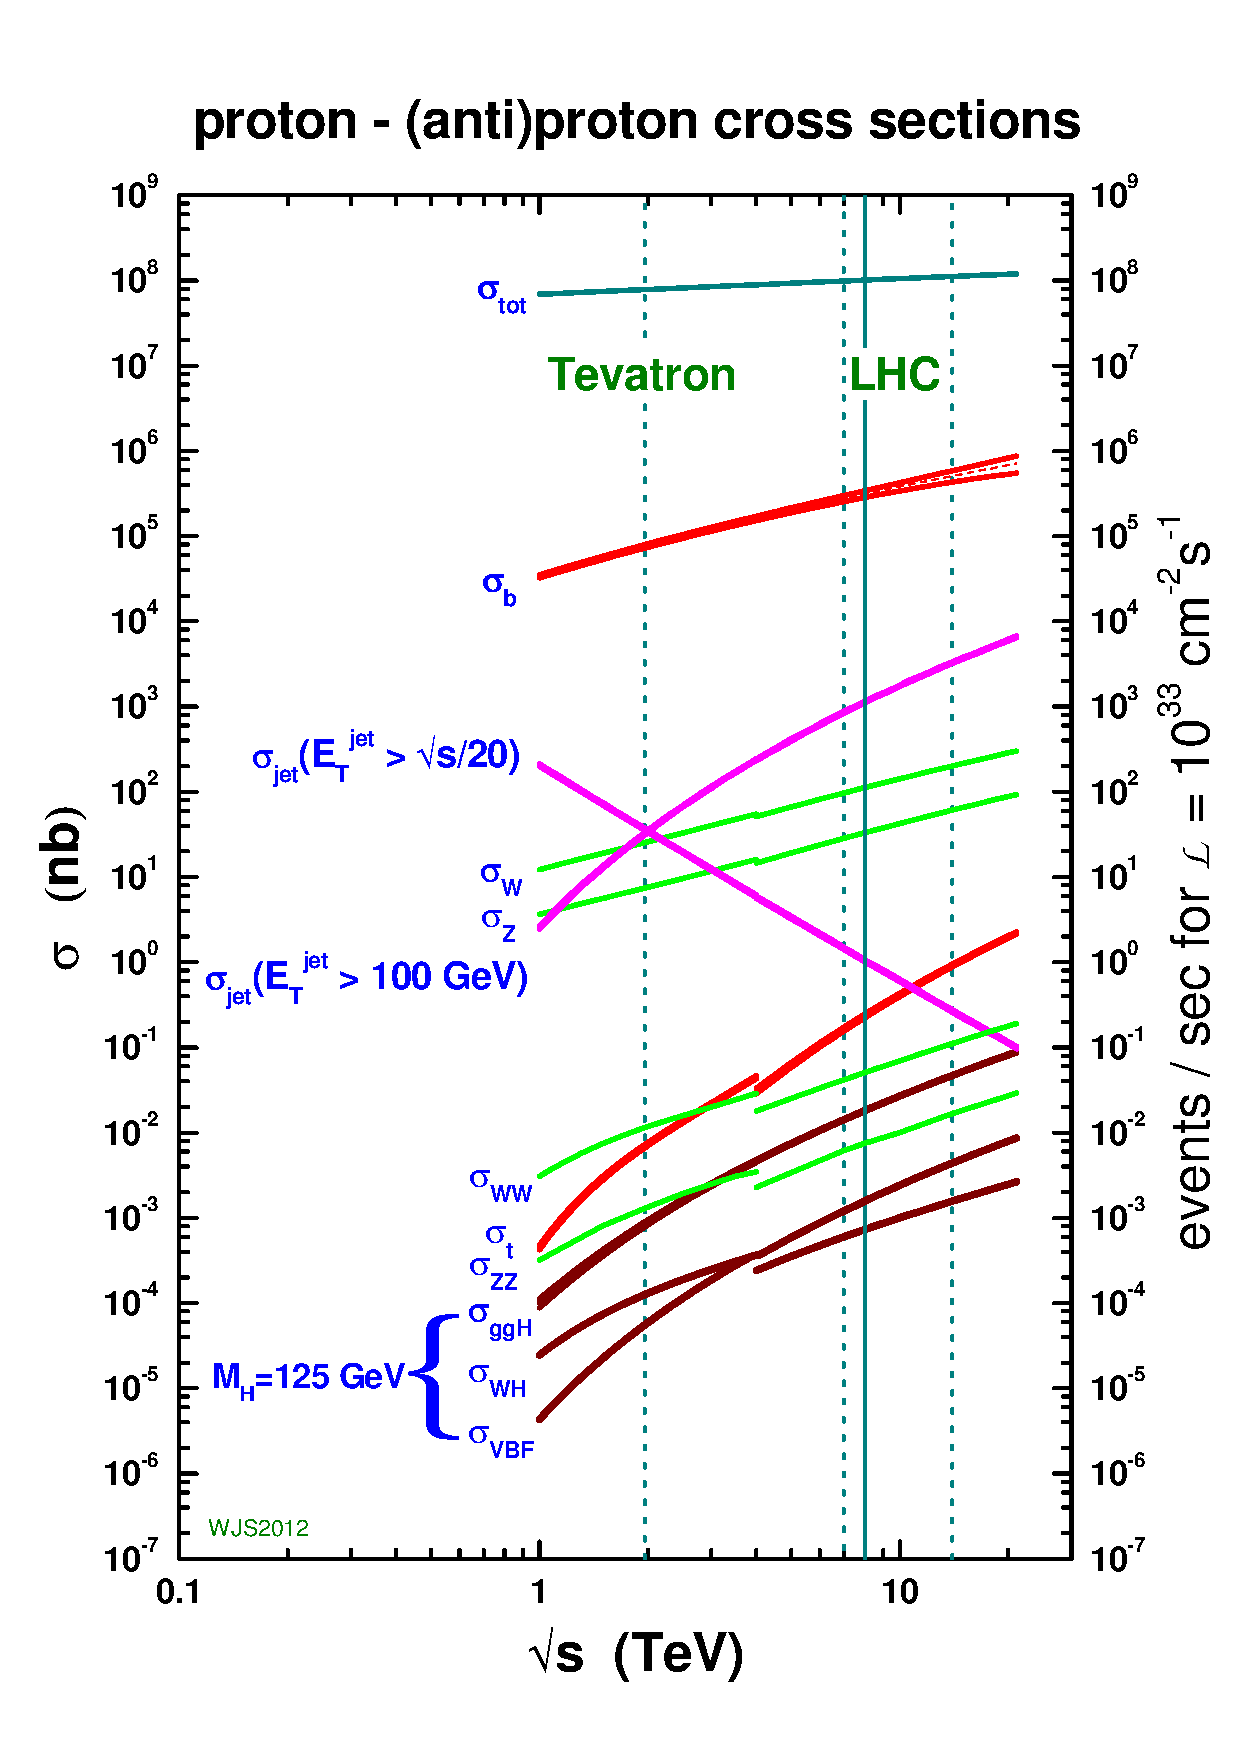
\includegraphics[scale=0.40]{./figures/crosssections2012_v5_LHC.pdf}
      \caption{Sections efficaces du mod\`ele standard lors de collisions $pp$ ou $p\overline{p}$ en fonction de l'\'energie dans le centre de masse. \`A droite est indiqu\'e le nombre d'\'ev\'enements par seconde correspondant \`a une luminosit\'e de $10^{33}cm^{-2}s^{-1}$}
     \label{fig:sect_eff_pp}
     \end{center}
  \end{figure}
   
   \medskip
   
   La figure \ref{fig:sect_eff_pp} indique les sections efficaces du mod\`ele standard de diff\'erents processus int\'eressants pour des collisions $pp$ ou $p\overline{p}$. Les sections efficaces de production du Higgs \`a 125 $GeV$ sont par exemple environ 10 \`a 11 ordres de grandeur inf\'erieur \`a la section efficace totale. Cela signifie qu'il faut pouvoir identifier un \'ev\'enement int\'eressant parmi $10^{11}$ \'ev\'enements de bruit de fond. De plus, \'etant donn\'e la section efficace \'elev\'ee, un nombre important d'\'ev\'enements par croisement de faisceau sont produits. Par exemple au LHC, avec la luminosit\'e de 2012, il y a eu environ 30 \'ev\'enements par croisement de faisceau (25 $ns$). Un syst\`eme perfectionn\'e de d\'eclenchement est donc n\'ecessaire pour pouvoir identifier le processus d\'esir\'e. Les d\'eclenchements ont alors lieux en fonction des caract\'eristiques des \'etats finaux recherch\'es. Les d\'etecteurs doivent aussi \^etre adapt\'es au fort niveau de radiations. Ainsi, une nouvelle particule ou un nouveau processus peut \^etre d\'ecouvert et \'etudi\'e si et seulement si le signal cr\'e\'e peut \^etre clairement identifi\'e au milieu des autres processus mis en jeu.

  \begin{figure}[!htb]
    \begin{center} 
      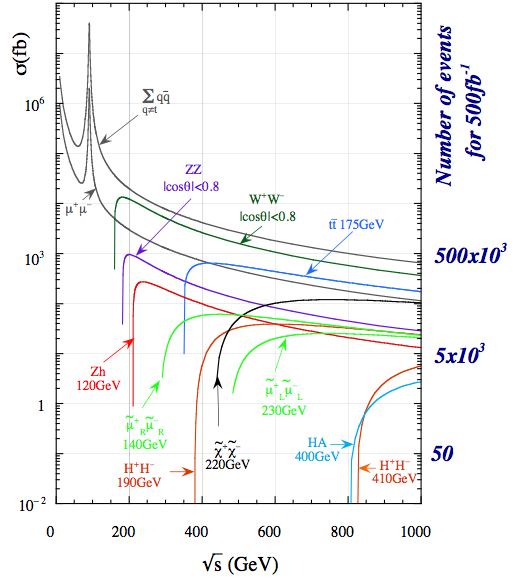
\includegraphics[scale=0.45]{./figures/JLC_physics_xsections.png}
      \caption{Sections efficaces du mod\`ele standard et de certaines particules supersym\'etriques lors de collision $e^+ e^-$ en fonction de l'\'energie dans le centre de masse. Le nombre d'\'ev\'enements correspondant \`a 500 $fb^{-1}$ de donn\'ees collect\'ees est indiqu\'e en bleu sur le côt\'e droit.}
     \label{fig:sect_eff_ee}
     \end{center}
  \end{figure}
   
   \medskip
   
   Voyons \`a pr\'esent la situation des collisionneurs $e^+$ $e^-$. La figure \ref{fig:sect_eff_ee} montre la section efficace de production de certains processus du mod\`ele standard et de la super-sym\'etrie pour des collisions $e^+$ $e^-$. Pour une \'energie disponible dans le centre de masse de 500 $GeV$, les processus physiques int\'eressants, comme la production de boson Higgs, de quark top ou de particules supersym\'etriques sont entre 0 et 2 ordres de grandeur inf\'erieurs \`a la section efficace totale. De plus, la section efficace de ces processus \`a 500 $GeV$ est environ comprise entre 10 et 100 $fb$. Il s'agit de sections efficaces beaucoup plus faibles, environ $10^4$ plus faibles, que celles obtenues lors de collisions $pp$ ou $p\overline{p}$. Cela autorise l'enregistrement de toutes les donn\'ees cr\'ees dans les d\'etecteurs sans syst\`eme de d\'eclenchement. Ainsi, tous les \'etats finaux sont enregistr\'es, pas seulement les plus caract\'eristiques, et toutes les donn\'ees sont disponibles pour l'analyse hors ligne. Cela implique que tous les processus et toutes les nouvelles particules sont pr\'esents dans les donn\'ees enregistr\'ees. Comme l'\'etat initial est connu avec pr\'ecision, la mesure de la masse manquante est alors r\'ealisable pr\'ecis\'ement. Il s'agit d'un atout consid\'erable lorsque l'on veut mesurer des particules n'interagissant que très peu. Cela permet de d\'ecouvrir des processus physiques non accessibles avec des collisionneurs $pp$ ou $p\overline{p}$. Dans un collisionneur hadronique comme celui du LHC, la mesure des rapports de branchement absolus et des largeurs totales n'est pas accessible directement, elles d\'ependent du mod\`ele de physique utilis\'e. Or, pour un collisionneur $e^+$ $e^-$, comme toutes les donn\'ees peuvent \^etre enregistr\'ees en raison du faible taux de production, et comme l'\'etat initial est pr\'ecis\'ement connu, il est possible de r\'ealiser des mesures ne d\'ependant d'aucun mod\`ele gr\^ace \`a la m\'ethode de la masse de recul. Il s'agit l\`a d'un atout non n\'egligeable. Non expliciterons cette m\'ethode dans la section \ref{sect:prog_physique}.
   
   \medskip
   
   Enfin, le probl\`eme de la calculabilit\'e des processus QCD est une limitation des collisionneurs hadroniques. Par exemple au LHC, les calculs des sections efficaces sont bas\'es sur la chromodynamique quantique (QCD). Or tout calcul th\'eorique portant sur le signal ou le bruit de fond a des incertitudes syst\'ematiques provenant : des fonctions de structure du proton, des corrections perturbatives d'ordre \'elev\'e, et des effets non perturbatifs QCD. Les corrections QCD \`a un ordre sup\'erieur (NLO) pour le calcul des sections efficaces sont de l'ordre de $30$ \`a $50\%$. Et en particulier pour le boson de Higgs la premi\`ere correction est de l'ordre de $100 \%$ ! Pour obtenir des erreurs inf\'erieures \`a $10 \%$, des calculs \`a des ordres encore sup\'erieurs (NNLO) sont n\'ecessaires. Étant donn\'e la complexit\'e des calculs, ce niveau de pr\'ecision n'est pas atteignable hormis pour les r\'eactions les plus simples. Pour les r\'eactions $e^+$ $e^-$, les électrons et positons sont des particules \'el\'ementaires, et elles n'interagissent que par interaction électrofaible. Les calculs sont dans ce cas l\`a beaucoup plus simples. Ainsi, les premi\`eres corrections radiatives sont de l'ordre de quelques pour-cents. Des calculs \`a des ordres encore plus grands peuvent \^etre effectu\'es pour atteindre une pr\'ecision th\'eorique de l'ordre du pour-mille. Ainsi, les comparaisons entre th\'eorie et résultats exp\'erimentaux sont facilit\'ees et pourrait permettre de d\'ecouvrir des d\'eviations signant la pr\'esence de nouvelle physique.
   
% Third and perhaps most importantly, at the ILC, it is much easier to
% recognize W and Z bosons in their hadronic decay modes than at the LHC. Since
% most W and Z decays are to hadronic modes, this is a tremendous advantage in the
% systematic study of heavy particles whose decay products typically include the weak
% bosons. We will see that this advantage applies not only to exotic particles but also
% in the study of the top quark and the Higgs boson.
  
   \medskip
   
   Malgr\'e leur plus faible \'energie disponible dans le centre de masse, les collisionneurs $e^+$ $e^-$ permettent des mesures plus pr\'ecises que les collisionneurs hadroniques. Ils permettent de plus de d\'etecter des \'ev\'enements qui ne seraient pas accessibles avec les collisionneurs $pp$ ou $p\overline{p}$. Cependant, les faibles sections efficaces de production doivent \^etre compens\'ees par une luminosit\'e \'elev\'ee. Il s'agit d'un d\'efi technologique dans le cas des acc\'el\'erateurs lin\'eaires. Avec la technologie actuelle, certains projets de collisionneurs $e^+$ $e^-$, comme celui de l'ILC, dot\'e d'une \'energie dans le centre de masse de 500 $GeV$ et d'une luminosit\'e nominale d'environ $10^{34} cm^{-2}s^{-1}$ sont r\'ealisables prochainement. De surcro\^it, les collisionneurs hadroniques permettent de sonder des gammes d'\'energies beaucoup plus importantes et permettent de cr\'eer des particules plus massives que celles d'un collisionneur $e^+$ $e^-$ dot\'e d'une \'energie dans le centre de masse plus faible. Cependant, les collisionneurs $e^+$ $e^-$ permettent de mesurer très pr\'ecis\'ement certains param\`etres fix\'es th\'eoriquement par la pr\'esence de particules beaucoup plus massives. Ils peuvent donc aussi d\'ecouvrir une physique nouvelle \`a plus haute \'energie.
  
  \FloatBarrier
  
  \subsection{D\'ecouverte du quark top et d'un nouveau boson}
  
  Postul\'e th\'eoriquement depuis les ann\'ees 70, et confirm\'e apr\`es la d\'ecouverte du quark b en 1977 au Fermilab, les diff\'erentes exp\'eriences de physique des particules, se sont mises \`a rechercher le quark top. C'est r\'ecemment, en 1995, que les exp\'eriences $CDF$ et $D\O{0}$ au Tevatron ont d\'ecouvert et mesur\'e les propri\'et\'es du quark top. \`A cette date, une combinaison des donn\'ees de ces deux exp\'eriences a abouti \`a la d\'etermination de la masse du quark top telle que $M_{top} = 176 \pm 8 \pm 10 \, GeV/c^2$ \cite{Abe:1995hr} et \`a celle de la section efficace  $\sigma_{t\overline{t}} = 6.8^{+3.6}_{-2.4} \, pb$ \cite{Abe:1995hr} \`a $\sqrt{s} = 1.8 \, TeV$. Plusieurs ann\'ees plus tard, le programme du Tevatron continuant, la statistique a augment\'ee et ces valeurs ont \'et\'e raffin\'ees. Puis, avec l'arriv\'ee des donn\'ees du LHC sur le quark top, de nouvelles valeurs plus pr\'ecises encore ont \'et\'e obtenues. Ainsi, avec une combinaison des donn\'ees du Tevatron et du LHC, la masse du quark top est maintenant estim\'ee \`a $m_{top} = 173.34 \pm 0.27 (stat) \pm 0.71 (syst) \, GeV/c^2$ \cite{ATLAS:2014wva}. La masse \'elev\'ee du quark top, quasi-équivalente \`a un noyau de tungst\`ene, et le rapport de sa masse par rapport \`a celle des autres quarks en font un objet myst\'erieux. La masse du quark top \'etant tr\`es \'elev\'ee, sa dur\'ee de vie moyenne pr\'edite par le mod\`ele standard est de l'ordre de $10^{-25} \, s$. En cons\'equence, le quark top n'hadronise pas. Il se d\'esint\`egre alors par le biais de l'interaction faible. Il se d\'esint\`egre dans presque $100 \%$ des cas en $W^{\pm}$ + quark b.
  
  \medskip

  Le (Un ?) boson de Higgs a quant \`a lui \'et\'e d\'ecouvert au LHC en 2012. L'annonce de la d\'ecouverte de ce nouveau boson par les exp\'eriences ATLAS \cite{Aad:2012tfa} et CMS \cite{Chatrchyan:2012ufa} a eu lieu le 4 juillet 2012 au CERN, quelques mois apr\`es que les premi\`eres preuves soit apparues. Ce jour l\`a, la collaboration ATLAS a mis en \'evidence la production d'un boson neutre dot\'e d'une masse de  $126.0 \pm 0.4 (stat) \pm 0.4 (sys) \, GeV/c^2$ avec un niveau de confiance donn\'e par $5.9$ \'ecarts standards. Ce nouveau boson est compatible avec le boson de Higgs du mod\`ele standard. La collaboration CMS a quant \`a elle trouv\'e un nouveau boson de masse $125.3 \pm 0.4 (stat.) \pm 0.5 (syst.) \, GeV/c^2$ avec une signification de $5.8$ \'ecarts standards. La d\'esint\'egration de ce nouveau boson dans la voie $\gamma \gamma$ indique que le spin de ce boson est diff\'erent de 1.
  
  \medskip
  
  \`A l'heure actuelle, les exp\'eriences ATLAS et CMS ont analys\'e les 25 $fb^{-1}$ de donn\'ees r\'ecolt\'ees \`a 7 et 8 $TeV$. Les r\'esultats obtenus par ATLAS \cite{Aad:2014aba} pour les canaux $H \rightarrow \gamma \gamma$ et $H \rightarrow Z Z^*  \rightarrow 4 l$ sont list\'es dans le tableau \ref{ATLAS_results_2014}. On retiendra comme valeur de la masse du Higgs \`a : $m_H = 125.36 \pm 0.41 \, GeV/c^2$.
  
  \begin{table}{
  \begin{center}
   \begin{tabular}{|l|l|l|} \hline
     Canal & {Masse mesur\'ee $[GeV/c^2]$} \\ \hline
     $H \rightarrow \gamma \gamma$ & $125.98 \pm 0.42 (stat) \pm 0.28 (syst) = 125.98 \pm 0.50$ \\ \hline
     $H \rightarrow Z Z^*  \rightarrow 4 l$ & $124.51 \pm 0.52 (stat) \pm 0.06 (syst) = 124.51 \pm 0.52$\\ \hline
     Combin\'e & $125.36 \pm 0.37 (stat) \pm 0.18 (syst) = 125.36 \pm 0.41$ \\ \hline
   \end{tabular}
   \caption{Masse du boson de Higgs mesur\'ee par ATLAS dans les canaux $H \rightarrow \gamma \gamma$ et $H \rightarrow Z Z^*  \rightarrow 4 l$. Avec 25 $fb^{-1}$ de donn\'ees collect\'ees}
   \label{ATLAS_results_2014}
  \end{center}}
 \end{table}
 
  \begin{figure}[!htb]
    \begin{center}
     \subfigure[Contours \`a $68\%$ d'intervalle de confiance pour le signal observ\'e divis\'e par le signal attendu dans le cas d'un Higgs standard, en fonction de la masse du Higgs mesur\'ee dans les canaux $H \rightarrow \gamma \gamma$ (vert) et  $H \rightarrow Z Z^*  \rightarrow 4 l$ (rouge). La courbe noire repr\'esente la combinaison des deux canaux. $\sigma/\sigma_{MS}$ est la section efficace de production multipli\'ee par le rapport de branchement correspondant divis\'ee par la valeur attendu par le mod\`ele standard. Le Higgs mesur\'e est compatible avec le Higgs du mod\`ele standard. \cite{Aad:2014aba}]{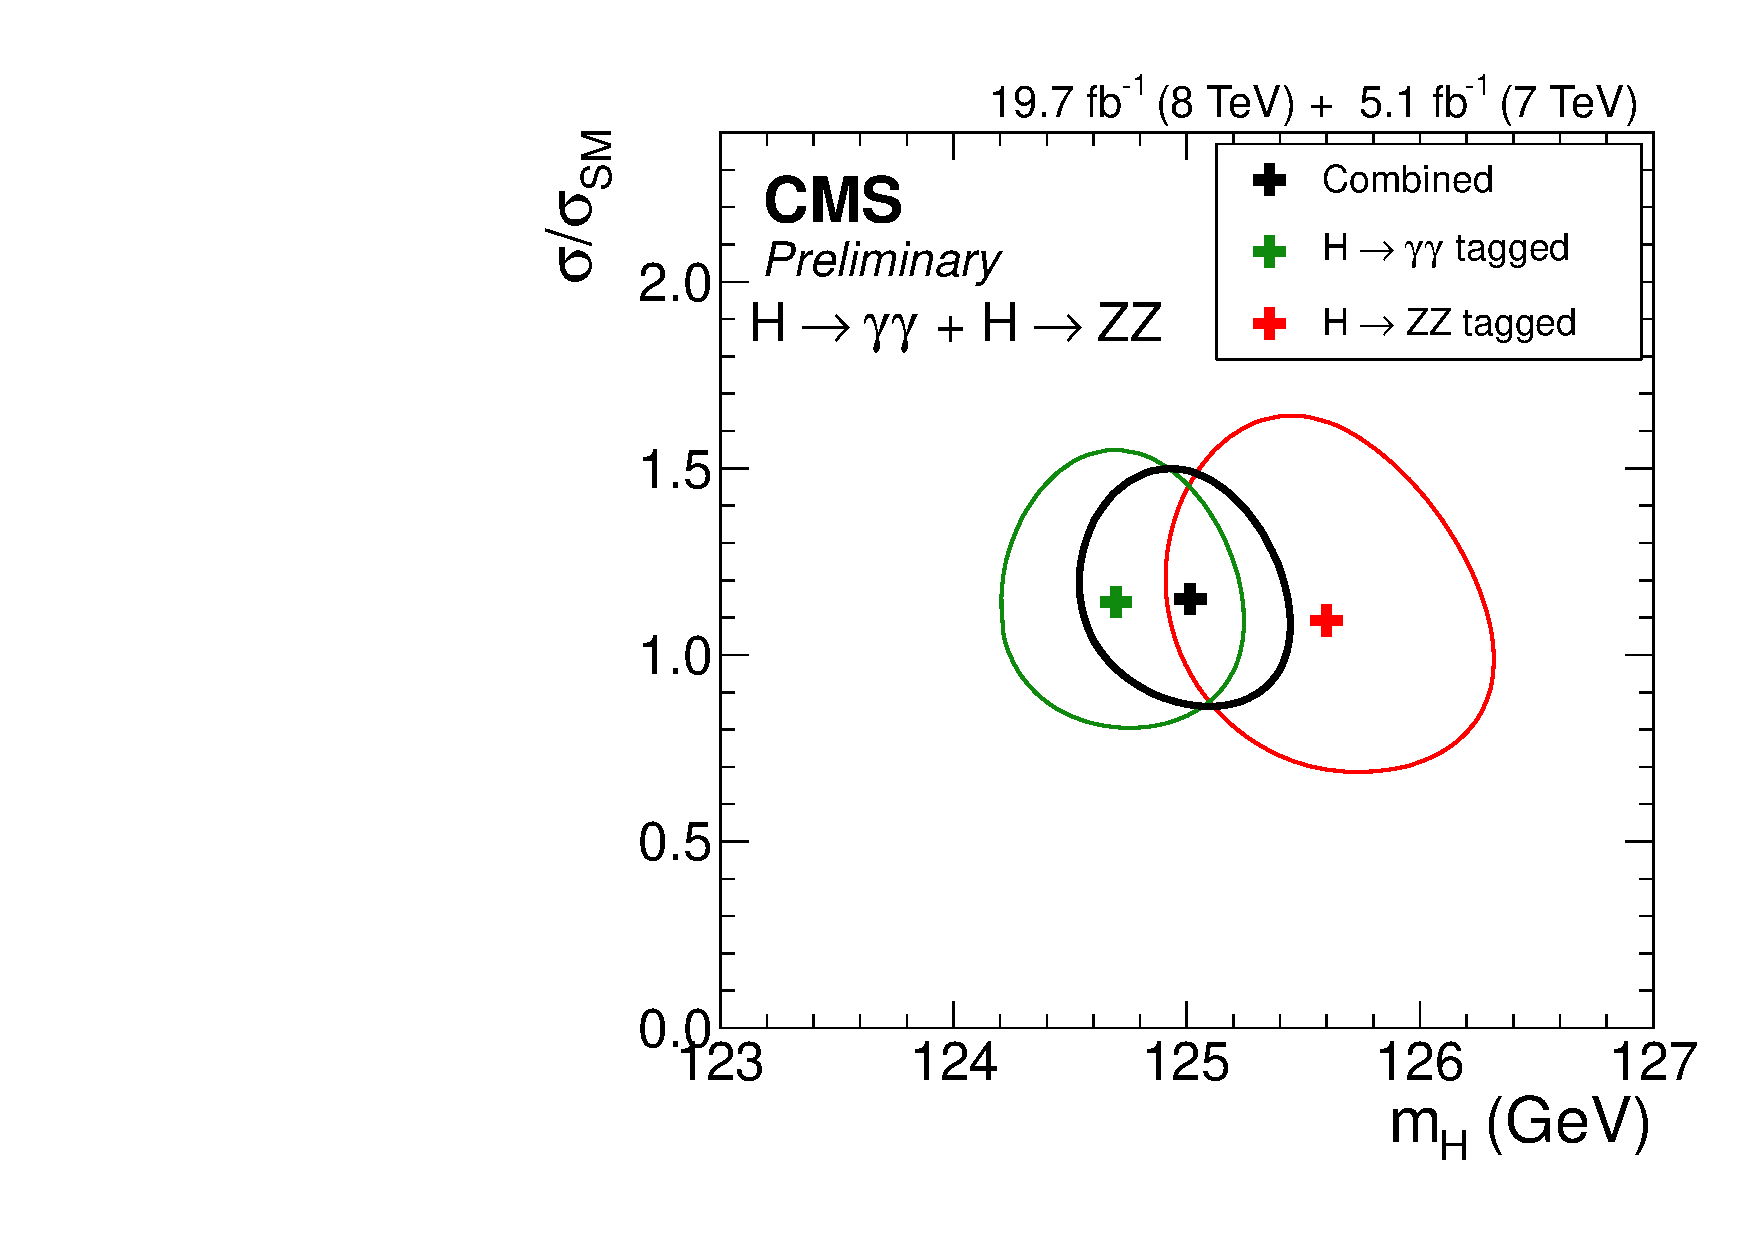
\includegraphics[scale=0.32]{./figures/CMS_Higgs_2014.pdf} }\quad
     \subfigure[Contours \`a $68\%$ et $95\%$ d'intervalle de confiance pour le signal observ\'e divis\'e par le signal attendu dans le cas d'un Higgs standard, en fonction de la masse du Higgs mesur\'ee dans les canaux $H \rightarrow \gamma \gamma$ (rouge) et  $H \rightarrow Z Z^*  \rightarrow 4 l$ (bleu). La courbe noire repr\'esente la combinaison des deux canaux. $\sigma/\sigma_{MS}$ est la section efficace de production multipli\'ee par le rapport de branchement correspondant divis\'ee par la valeur attendu par le mod\`ele standard. Le Higgs mesur\'e est compatible avec le Higgs du mod\`ele standard. \cite{CMS-PAS-HIG-14-009}]{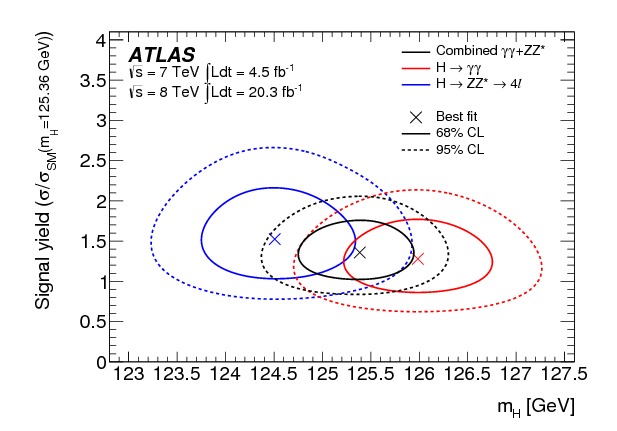
\includegraphics[scale=0.35]{./figures/ATLAS_Higgs_mu_vs_mh_no_mh_dep.png} }
    \end{center}
    \caption{}
    \label{fig:CMS_ATLAS}
  \end{figure}
 
  CMS avec les m\^emes canaux et 25 $fb^{-1}$ de donn\'ees analys\'ees mesure une masse de $m_H = 125.03^{+0.26}_{-0.27} (stat.) ^{+0.13}_{-0.15} (syst.) \, GeV/c^2$ \cite{CMS-PAS-HIG-14-009}. La figure \ref{fig:CMS_ATLAS} illustre ces nouvelles valeurs de masse analys\'ees par les exp\'eriences ATLAS et CMS et compare les signaux obtenus \`a ceux pr\'evus pour un Higgs du mod\`ele standard.
  
%  et \ref{fig:CMS_new}

  \begin{figure}[!htb]
    \begin{center} 
      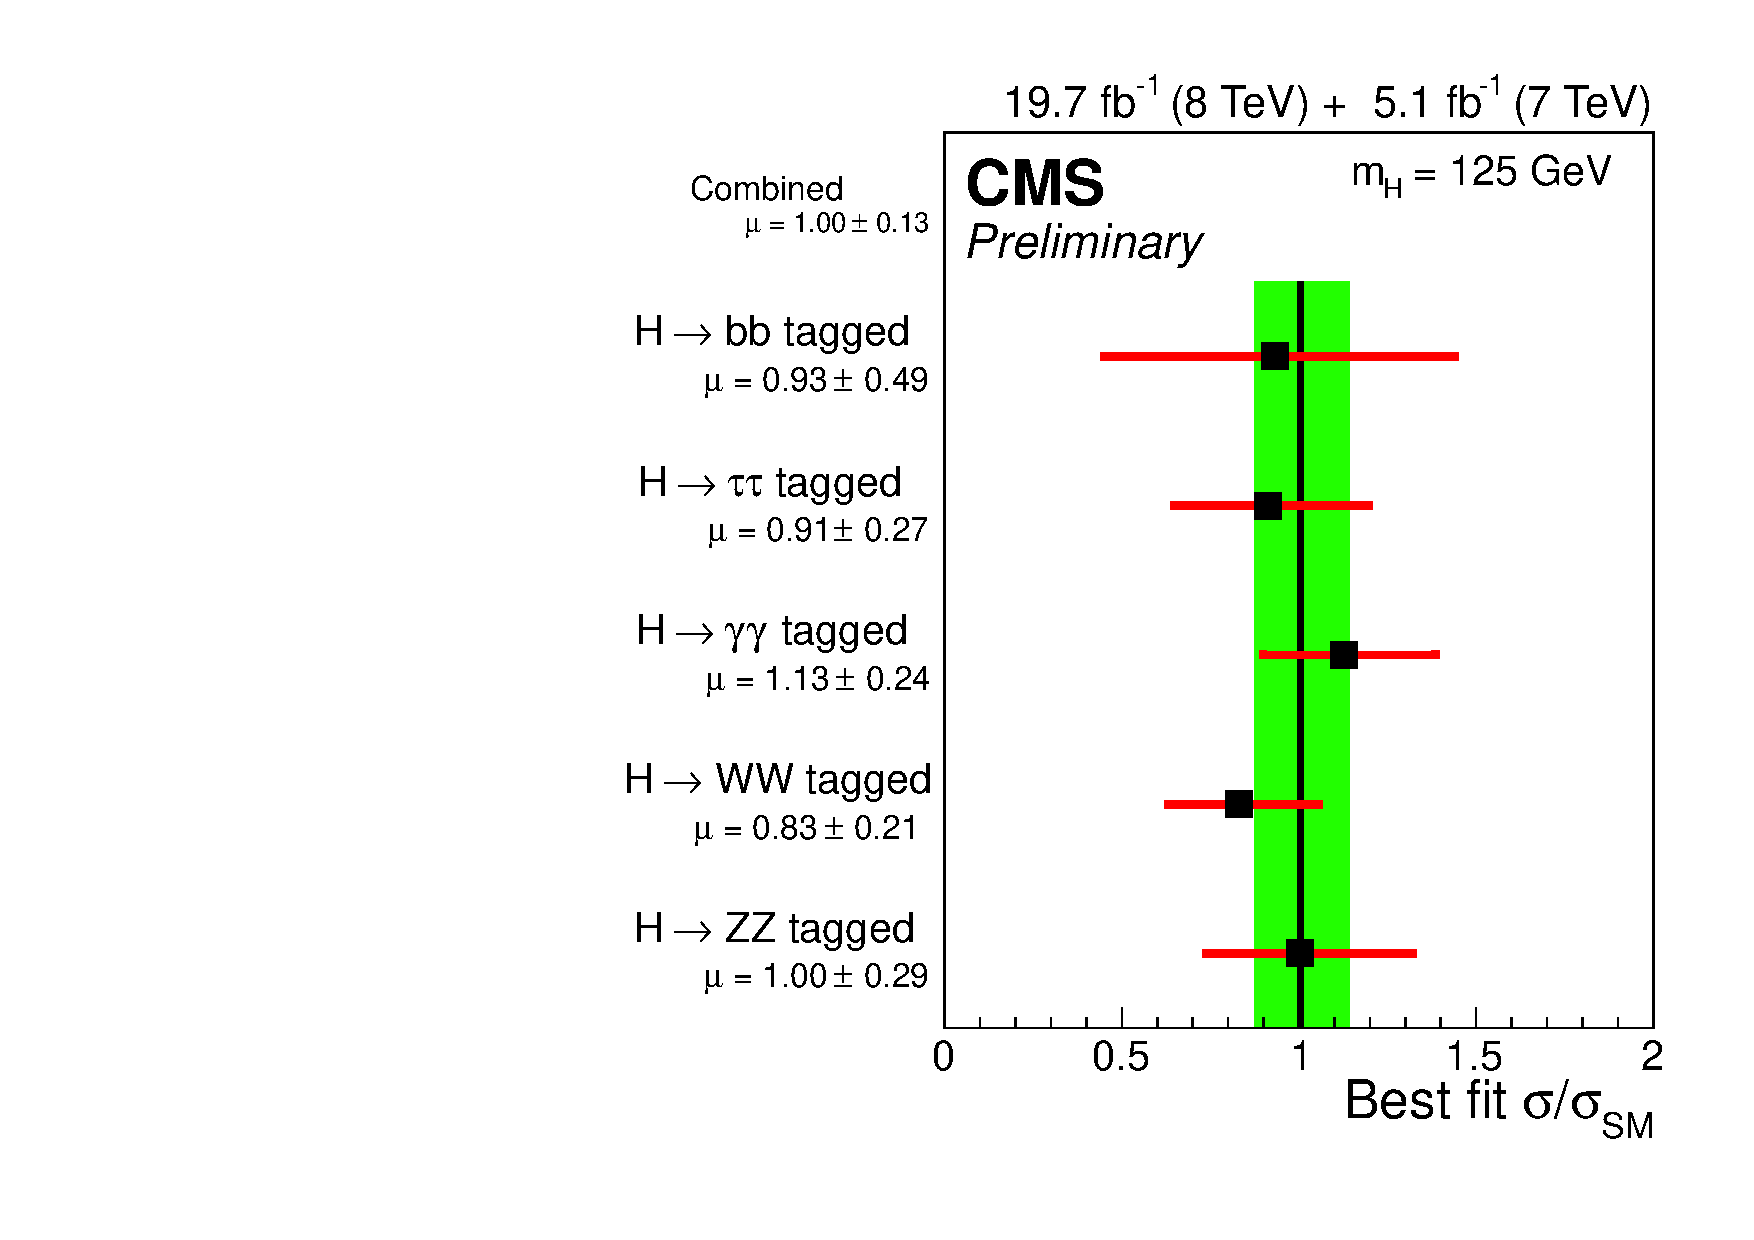
\includegraphics[scale=0.45]{./figures/Higgs_decay_CMS.pdf}
      \caption{Sections efficaces de d\'esint\'egration du Higgs selon les diff\'erents canaux mesur\'es par l'exp\'erience CMS rapport\'ees \`a celle pr\'evues par le mod\`ele standard. \cite{CMS-PAS-HIG-14-009}}
     \label{fig:CMS_decay_Higgs}
     \end{center}
  \end{figure}

%   \begin{figure}[!htb]
%     \begin{center} 
%       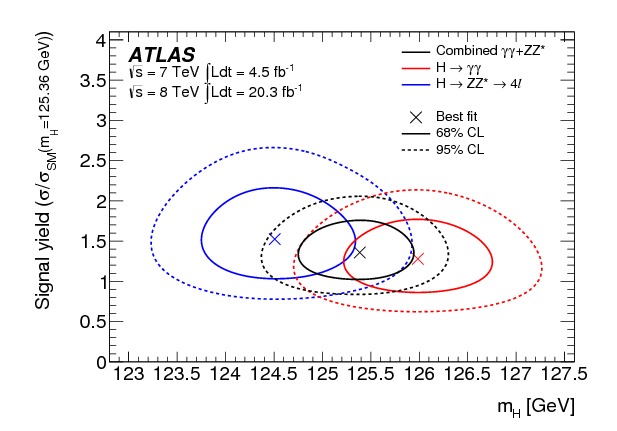
\includegraphics[scale=0.50]{./figures/ATLAS_Higgs_mu_vs_mh_no_mh_dep.png}
%       \caption{Contours \`a $68\%$ et $95\%$ d'intervalle de confiance pour le signal observ\'e divis\'e par le signal attendu dans le cas d'un Higgs standard, en fonction de la masse du Higgs mesur\'ee dans les canaux $H \rightarrow \gamma \gamma$ (rouge) et  $H \rightarrow Z Z^*  \rightarrow 4 l$ (bleu). La courbe noir repr\'esente la combinaison des deux canaux. $\sigma/\sigma_{MS}$ est la section efficace de production multipli\'ee par le rapport de branchement correspondant divis\'ee par la valeur attendu par le mod\`ele standard. Le Higgs mesur\'e est compatible avec le Higgs du mod\`ele standard}
%      \label{fig:ATLAS_new}
%      \end{center}
%   \end{figure}
%   
%   \begin{figure}[!htb]
%     \begin{center} 
%       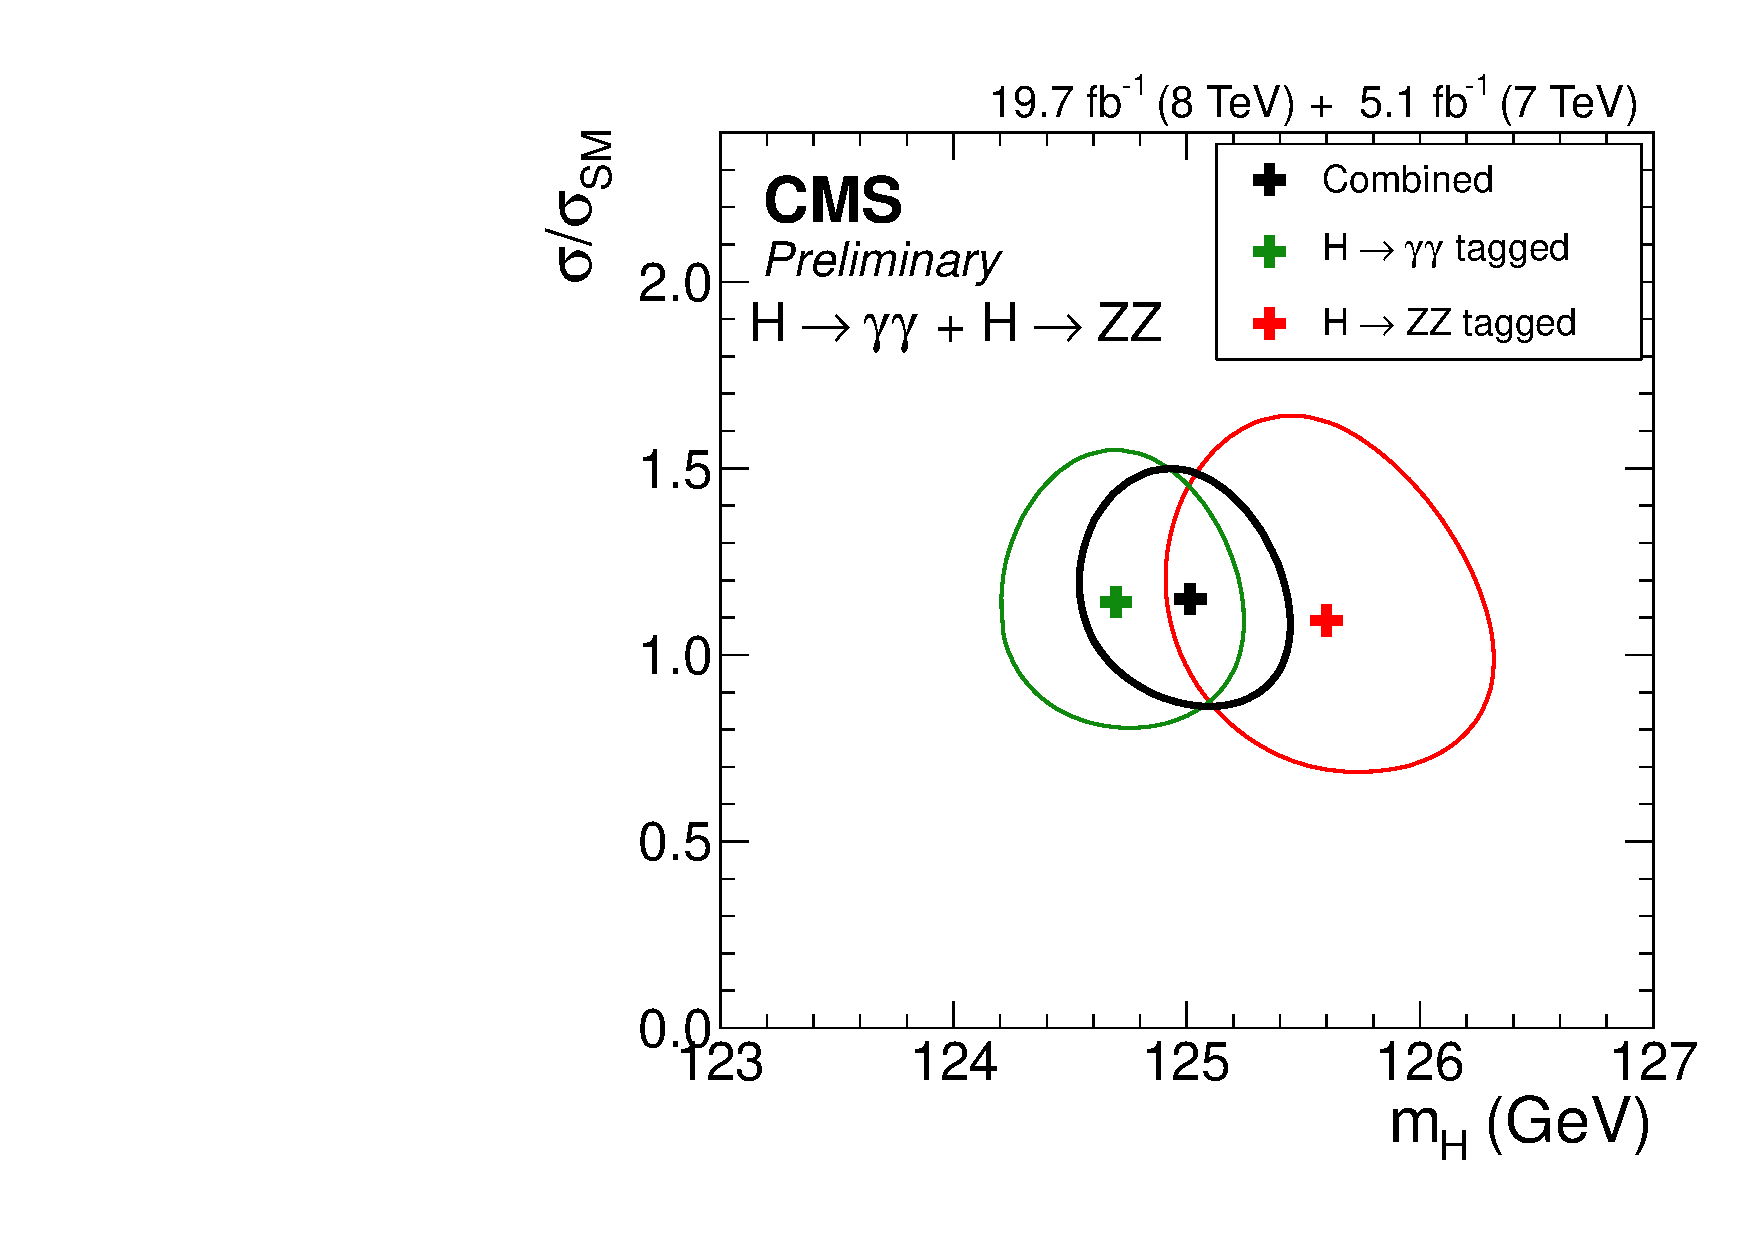
\includegraphics[scale=0.50]{./figures/CMS_Higgs_2014.pdf}
%       \caption{Contours \`a $68\%$ d'intervalle de confiance pour le signal observ\'e divis\'e par le signal attendu dans le cas d'un Higgs standard, en fonction de la masse du Higgs mesur\'ee dans les canaux $H \rightarrow \gamma \gamma$ (vert) et  $H \rightarrow Z Z^*  \rightarrow 4 l$ (rouge). La courbe noir repr\'esente la combinaison des deux canaux. $\sigma/\sigma_{MS}$ est la section efficace de production multipli\'ee par le rapport de branchement correspondant divis\'ee par la valeur attendu par le mod\`ele standard. Le Higgs mesur\'e est compatible avec le Higgs du mod\`ele standard}
%      \label{fig:CMS_new}
%      \end{center}
%   \end{figure}

  \medskip

  De plus, certaines sections efficaces de diff\'erentes voies de d\'esint\'egration du Higgs ont aussi pu \^etre mesur\'ees. La figure \ref{fig:CMS_decay_Higgs} pr\'esente les r\'esultats de CMS montrant l'\'ecart des sections efficaces de d\'esint\'egration du Higgs mesur\'ees par rapport aux sections efficaces th\'eoriques du mod\`ele standard. D'apr\`es ces r\'esultats le boson trouv\'e est compatible avec un boson de Higgs standard. Au niveau du spin et de la parit\'e, un spin $0$ est favoris\'e avec une parit\'e positive \cite{Aad:2013xqa}. Pour plus d'informations, un r\'esum\'e des r\'esultats obtenus par les exp\'eriences ATLAS et CMS jusqu'à l'\'et\'e 2014 est disponible dans la r\'ef\'erence \cite{Wang:2014xsa}.
  
  \medskip
  
  Les r\'esultats que nous avons pr\'esent\'es pour le Higgs devrait \^etre am\'elior\'es durant la seconde phase de fonctionnement du LHC (Run2). La prise de donn\'ees pour cette seconde phase d\'ebutera \`a l'\'et\'e 2015. Cette fois-ci l'\'energie dans le centre de masse sera de 13 puis 14 $TeV$. Cette seconde phase s'arrêtera mi-2017. D\'ebutera alors un long arrêt jusqu'\`a mi-2018, date \`a laquelle la troisième phase (Run3) devrait d\'ebuter. Cette phase durera jusqu'à fin 2020 d\'ebut 2021. A la fin des trois phases de fonctionnement du LHC, la luminosit\'e int\'egr\'ee atteindra environ 300 \`a 350 $fb^{-1}$. Cela permettra d'affiner les pr\'ecisions sur les mesures d\'ejà existantes et on l'esp\`ere de d\'ecouvrir de nouvelles particules. Les arr\^ets inter-phases permettront la mise \`a jour de l'acc\'el\'erateur et de certains d\'etecteurs. \`A partir de 2023, \textit{HL-LHC} pour \textit{High Luminosity Large Hadron Collider}, une extension du LHC fournissant une plus haute luminosit\'e est en projet. Le projet pourrait fournir une luminosit\'e int\'egr\'ee d'environ 3000 $fb^{-1}$ en dix ann\'ees de fonctionnement.
  
  \begin{figure}[!htb]
    \begin{center} 
      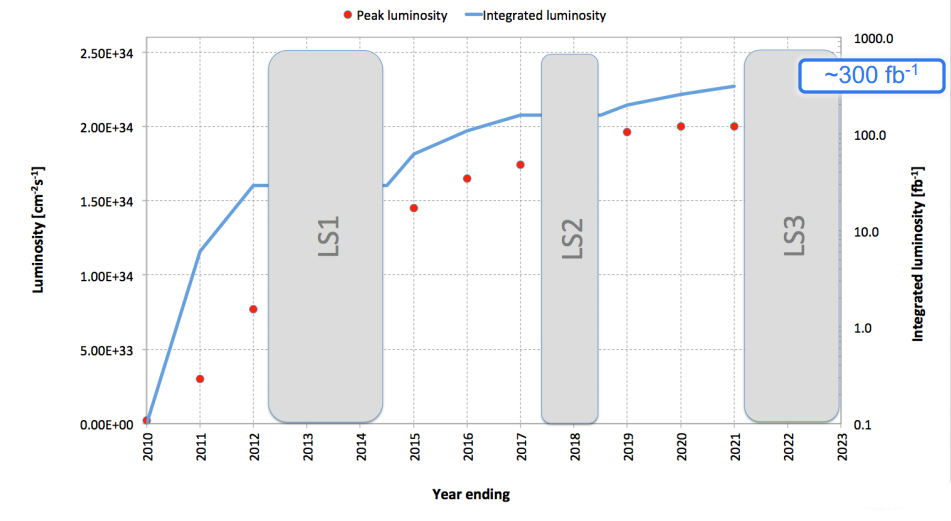
\includegraphics[scale=0.30]{./figures/program_LHC.png}
      \caption{Les diff\'erentes phases du LHC en fonction de la luminosit\'e de l'acc\'el\'erateur.}
     \label{fig:program_LHC}
     \end{center}
  \end{figure}
  
  \medskip
  
  Pour conclure, de nombreuses questions restent en suspens au sujet du quark top et du boson de Higgs. Des mesures de pr\'ecision devraient permettre de repousser les limites de notre compréhension sur ces deux particules en particulier. Le boson de Higgs d\'ecouvert au LHC est-il standard ? existe-t-il plusieurs bosons de Higgs comme dans les th\'eories supersym\'etriques ? Pourquoi le quark top poss\`ede-t-il une masse si \'elev\'ee ? Le LHC et de nouveaux collisionneurs devraient permettre d'apporter des \'el\'ements de r\'eponses \`a ces questions. Une liste non exhaustive des collisionneurs du futur, actuellement en projet, est donn\'ee dans la section suivante.
  
%   accelerateur hadronique pas assez precis ? \\
%   Mesures de pr\'ecsions pourquoi faire ? \\
%   Nombres quantiques et couplages du Higgs :) \\
%   Physique du top \\
%   en compl\'ementarit\'e avec le LHC. \\
  
  \FloatBarrier
  
  \subsection{Les collisionneurs du futur}
  
  Dans cette partie nous allons pr\'esenter les diff\'erents projets de collisionneurs de particules de demain. Il s'agit d'une revue non exhaustive des possibilit\'es \`a l'\'etude en 2015. Depuis 2012, le nouveau boson d\'ecouvert au LHC, est \'etudi\'e par la communaut\'e LHC. Comme nous l'avons vu plus haut, les exp\'eriences ATLAS et CMS analysent les donn\'ees d\'ej\`a disponibles afin de caract\'eriser le boson de Higgs et sa physique. Ce programme va s'entendre au moins jusque dans les ann\'ees 2020 comme mentionn\'e plus haut. 300 \`a 350 $fb^{-1}$ seront r\'ecolt\'es et permettrons d'\'etudier finement les propri\'et\'es du boson de Higgs, et espérons-le une physique nouvelle. Le HL-LHC devrait permettre de r\'ecolter environ $3000 \, fb^{-1}$ de donn\'ees. Cependant, même avec cette quantit\'e importante de donn\'ees, les param\`etres du boson trouv\'e récemment au LHC, comme sa masse, sa largeur ou ses couplages ne seront pas connus avec une grande pr\'ecision. De plus, comme nous l'avons vu plus haut, outre le fait qu'il fournisse des mesures moins pr\'ecises, le LHC est limit\'e dans certaines de ses d\'ecouvertes. L'\'evolution naturelle de la discipline de la physique des particules, amène \`a la construction de collisionneurs plus puissants ou plus pr\'ecis, permettant l'exploration d'une nouvelle physique en passant par l'augmentation de la gamme d'\'energie des faisceaux ou en passant par des mesures de pr\'ecisions, permettant de nouvelles d\'ecouvertes. Ainsi, dans les d\'ecennies \`a venir, un collisionneur $e^+$ $e^-$ est n\'ecessaire afin de mesurer, avec une pr\'ecision sup\'erieure \`a celle du LHC, le secteur \'electrofaible et sa brisure spontan\'ee, mais aussi la nouvelle physique \`a l'\'echelle du $TeV$. Dans la lign\'ee, des collisionneurs $pp$ dot\'es d'une \'energie dans le centre de masse allant jusqu'\`a 100 $TeV$ pourrait \^etre envisag\'es. Dans cette section nous d\'ecrirons les projets d'acc\'el\'erateurs du futur et nous introduirons l'ILC. C'est dans le contexte de l'ILC que s'ins\`ere cette th\`ese.
  
  \subsubsection{Futurs projets de collisionneurs}

  Nous allons ici décrire les principaux projets de collisionneurs du futur. Nous d\'ecrirons dans un premier temps les projets de collisionneurs lin\'eaires puis nous d\'ecrirons les derniers projets de collisionneurs circulaires \`a l'\'etude en Europe et en Chine. 
  
  \medskip
  
  Depuis quelques ann\'ees, deux projets de collisionneurs lin\'eaires $e^+$ $e^-$ sont \`a l'\'etude, il s'agit de l'ILC pour \textit{International Linear Collider} et de CLIC pour \textit{Compact Linear Collider}. Le premier utilise une technologie acc\'el\'eratrice bas\'ee sur des cavit\'es Radio-Fréquence super-conductrices. La limite actuelle du gradient d'acc\'el\'eration d'une telle technologie est d'environ 60 $MV/m$. Pour l'ILC  des cavit\'es de 31.5 $MV/m$ en moyenne sont envisag\'ees. L'\'energie nominale dans le centre de masse sera de 500 $GeV$ et une extension \`a 1 $TeV$ est pr\'evue. La luminosit\'e sera de $2 \times 10^{34} cm^{-2}s^{-1}$ \`a 500 $GeV$. L'ILC dans sa version 500 $GeV$ devrait mesurer 31 $km$ de long. 
  
  \medskip
  
  Pour pouvoir obtenir des champs acc\'el\'erateurs de l'ordre de ceux pr\'evus pour l'ILC, il faut injecter une onde radiofr\'equence dans la cavit\'e. Des courants de l'ordre de $10^{10}$ \`a $10^{12}$ $A/m^2$ circulent sur la surface interne de la cavit\'e et provoquent un échauffement des parois. On ne pourrait pas obtenir de champs aussi \'elev\'es en continu avec un conducteur normal. En effet, les parois se mettraient \`a fondre. En radio-fr\'equence, la r\'esistance d'un supra-conducteur n'est pas rigoureusement nulle, mais elle reste environ $10^5$ fois plus faible que celle du cuivre, d'o\`u l'intérêt principal de cette technologie pour les cavités accélératrices. 
  
  \medskip
  
  Du cot\'e de CLIC, l'objectif est d'arriver \`a des gradients d'acc\'el\'eration de l'ordre de 100 $MV/m$ afin de fournir une \'energie dans le centre de masse minimale de 500 $GeV$ et pouvant monter jusqu'\`a 5 $TeV$. L'acc\'el\'erateur est optimis\'e pour une \'energie de 3 $TeV$ dans le centre de masse et une luminosit\'e de $2 \, 10^{34} cm^{-2}s^{-1}$. Sa longueur dans sa version nominale \`a 3 $TeV$ serait d'environ 40 km de longueur. Un gradient de 100 $MV/m$ n'est pas atteignable \`a l'aide de cavit\'es radio-fr\'equence. Ainsi, une autre strat\'egie d'acc\'el\'eration est \`a l'\'etude pour atteindre un tel gradient.
  
  \medskip
  
  Pour atteindre un champ acc\'el\'erateur d'environ 100 $MV/m$, il faut pouvoir injecter des ondes de fr\'equence 12 $GHz$ \`a temp\'erature ambiante. Les klystrons (injecteurs de puissance) ne permettent pas d'injecter une telle puissance. Une solution d'acc\'el\'eration \`a deux faisceaux a alors \'et\'e d\'evelopp\'ee. Un premier faisceau dot\'e d'un fort courant d'\'electron de faible \'energie (de l'ordre de 9.0 $GeV$) appel\'e \textit{faisceau conducteur} est plac\'e parall\`element au faisceau principal. Puis, ce faisceau conducteur est d\'ec\'el\'er\'e dans une structure dite d'extraction de puissance (PETS) et la puissance g\'en\'er\'ee est transf\'er\'ee au faisceau principal. Un gradient d'acc\'el\'eration de l'ordre de 100 MV/m est alors cr\'e\'e.
  
  \medskip
  
  La technologie utilis\'ee dans le projet CLIC n'est pas encore mature. Un rapport d'\'elaboration conceptuel \textit{CDR} a \'et\'e remis en 2012 et un rapport technique de conception \textit{TDR} est pr\'evu pour 2018. Le projet ILC est quant \`a lui envisageable prochainement et diff\'erentes \'etapes ont d\'ej\`a été franchies vers sa conception. Un \textit{TDR}, est d\'ej\`a disponible depuis 2013. De plus, un site d'implantation a déjà \'et\'e avanc\'e, celui de \textit{Kitakami} au nord du Japon. L'ILC pourrait voir ses premiers faisceaux se collisionner au alentours de 2030. Nous reviendrons plus en d\'etail sur l'ILC dans la section suivante.
  
  \medskip
  
  Tr\`es récemment des \'etudes de futurs collisionneurs circulaires (FCC) ont vu le jour. Ces nouveaux projets d'acc\'el\'erateurs sont actuellement \`a l'\'etude en Europe (CERN) et en Chine.  Ils sont organis\'es en trois types de collisionneurs : les FCC-ee, les FCC-hh et les FCC-he.
  
  \medskip
  
  Du côt\'e du CERN, un nouvel anneau de 80-100 $km$ de circonf\'erence pourrait accueillir un collisionneur proton-proton dot\'e d'une \'energie de 100 TeV dans le centre de masse. Ce concept d'acc\'el\'erateur est nomm\'e \textit{FCC-hh} ou encore \textit{VHE-LHC} (pour \textit{Very High Energy Large hadron Collider}). Les 100 $TeV$ dans le centre de masse devraient permettre de tester et d\'ecouvrir de la nouvelle physique \`a tr\`es haute \'energie. Ce concept demande notamment des avanc\'ees technologiques afin de pouvoir concevoir et utiliser des aimants supra-conducteurs d'environ 20 Teslas. Ce collisionneur $hh$, pourrait \^etre pr\'ec\'ed\'e d'un autre collisionneur, $e^+$ $e^-$ cette fois-ci, fonctionnant \`a 4 \'energies dans le centre de masse distinctes afin de produire des mesures de pr\'ecision des bosons $Z$ ($\approx 90 \, GeV$) et $W$ ($\approx 160 \, GeV$), du boson de $Higgs$ ($\approx 240 \, GeV$) et du quark $top$ ($\approx 350 \, GeV$). Ce concept est nomm\'e \textit{FCC-ee} ou \textit{TLEP} pour \textit{Triple LEP}. Ce type de collisionneur demande de nombreux efforts de recherches et d\'eveloppements afin de poss\'eder les technologies n\'ecessaires. Un collisionneur hybride lepton-hadron (\textit{FCC-he}) constitue une autre option possible. De plus amples informations au sujet de ces projets sont disponibles dans un compte-rendu de la conf\'erence IPAC2014 \cite{Benedikt:1742294}. La remise d'un \textit{CDR} est pr\'evue pour 2018 en Europe. La mise en fonctionnement d'un de ces acc\'el\'erateurs pourrait avoir lieu, au plus tôt, pour les ann\'ees 2040.
  
  \medskip
  
  Du côt\'e chinois, des \'etudes similaires sont établies en parall\`ele du CERN. Un collisionneur $e^+$ $e^-$ nomm\'e \textit{CECP}, pour \textit{Circular Electron Positron Collider}, suivi d'un collisionneur $pp$ nomm\'e \textit{SppC}, pour \textit{Super pp Collider}, sont à l`'\'etude. Le \textit{CECP} serait un collisionneur circulaire h\'eberg\'e dans un tunnel de 50 \`a 70 kms de circonf\'erence, dot\'e de deux d\'etecteurs, plac\'es aux deux points d'interaction des faisceaux. L'\'energie dans le centre de masse est estim\'ee \`a 240-250 $GeV$, et la luminosit\'e \`a $2 \, 10^{34} cm^{-2}s^{-1}$. Le programme de physique serait proche de celui de \textit{TLEP}. Ensuite, dans un second temps, apr\`es l'exploitation du \textit{CECP}, le \textit{SppC} devrait prendre naissance dans le m\^eme tunnel. Il pourra d\'elivrer des collisions $pp$ avec une \'energie disponible dans le centre de masse de 50 \`a 70 $TeV$. La planification actuelle (septembre 2014) est la suivante. Un \textit{CDR} devrait pouvoir \^etre d\'elivr\'e fin 2014. Puis, des efforts de R\&D seront fournis entre 2016 et 2020, rendant possible la publication d'un \textit{TDR} aux alentours de 2020. Le planning de conception est le suivant : le \textit{CEPC} devrait \^etre construit entre 2021 et 2027. Le programme de physique devrait alors avoir lieu entre 2028 et 2035. La R\&D du \textit{SppC} s'\'etendra alors entre 2020 et 2030. La machine serait alors construite entre 2035 et 2042 dans le m\^eme tunnel que le \textit{CEPC}. Et le \textit{SppC} serait pr\^et \`a prendre des donn\'ees en 2042.
  
  \medskip
  
\newcommand{\ZH}{$ZH$}
\newcommand{\nnH}{ $\nu \bar{\nu} H$}
\newcommand{\nnHH}{ $\nu \bar{\nu} HH$}

\begin{table}[htb!]
\begin{center}
\tiny
\begin{tabular}{l|cc|cc|cc|c} \hline\hline
                        & \multicolumn{2}{c|}{ILC}                   & \multicolumn{2}{c|}{ILC LumiUp}                   & \multicolumn{2}{c|}{CLIC}              & \multicolumn{1}{c}{TLEP} \\
		        & \multicolumn{2}{c|}{250/500/1000 GeV}      & \multicolumn{2}{c|}{250/500/1000 GeV}             & \multicolumn{2}{c|}{1.4/3.0 TeV}       & \multicolumn{1}{c}{240 \& 350~GeV} \\ \hline
		        & \ZH            & \nnH & \ZH            & \nnH                 &  \ZH       &        \nnH           &  \ZH $(\nu\bar{\nu}H)$     \\ \hline
Inclusive              & 2.6/3.0/$-$\%  &  $-$ & 1.2/1.7/$-$\%  &  $-$                 &  4.2\%       &  $-$                  &  0.4\%              \\
$H\to \gamma\gamma$    & 29-38\%        & $-$/20-26/7-10\% & 16/19/$-$\%     & $-$/13/5.4\%           &  $-$           &  11\%/$<11$\%        &  3.0\%   \\
$H\to gg$              & 7/11/$-$\%     & $-$/4.1/2.3\% & 3.3/6.0/$-$\%      & $-$/2.3/1.4\%            &  6\%    &  1.4/1.4\%            &  1.4\%    \\
$H\to ZZ^*$            & 19/25/$-$\%    & $-$/8.2/4.1\% & 8.8/14/$-$\%       & $-$/4.6/2.6\%            &         &  2.3/1.5\%            &  3.1\% \\
$H\to WW^*$            & 6.4/9.2/$-$\%  & $-$/2.4/1.6\% & 3.0/5.1/$-$\%      & $-$/1.3/1.0\%            &  2\%    &  0.75/0.5\% &  0.9\%        \\
$H\to\tau\tau$         & 4.2/5.4/$-$\%  & $-$/9.0/3.1\%  & 2.0/3.0/$-$\%      & $-$/5.0/2.0\%            &  5.7\%         &  2.8\%/$<2.8$\%            &  0.7\%  \\
$H\to b\bar{b}$        & 1.2/1.8/$-$\%  & 11/0.66/0.30\% & 0.56/1.0/$-$\%    & 4.9/0.37/0.30\%          &  1\%    &  0.23/0.15\%          &  0.2\%  (0.6\%)    \\
$H\to c\bar{c}$        & 8.3/13/$-$\%   & $-$/6.2/3.1\% & 3.9/7.2/$-$\%      & $-$/3.5/2.0\%            &  5\%    &  2.2/2.0\%            &  1.2\%    \\
$H\to \mu\mu$          & $-$            & $-$/$-$/31\%  & $-$            & $-$/$-$/20\%              &  $-$           &  21/12\%    &  13\%        \\
\hline
& \multicolumn{2}{c|}{$t\bar{t}H$} & \multicolumn{2}{c|}{$t\bar{t}H$}        & \multicolumn{2}{c|}{$t\bar{t}H$}         & \multicolumn{1}{c}{$t\bar{t}H$} \\
\hline
$H\to b\bar{b}$        & \multicolumn{2}{c|}{$-$/28/6.0\%} & \multicolumn{2}{c|}{$-$/16/3.8\%}        & \multicolumn{2}{c|}{8\%/$<8$\%}   &  \multicolumn{1}{c}{$-$}  \\
\hline\hline
\end{tabular}
\caption{ \footnotesize{Pr\'ecision sur les sections efficaces $\sigma \cdot {\rm BR}$ mesur\'ees pour les futurs collisionneurs $e^+$ $e^-$. Sont indiqu\'es les pr\'ecisions pour les programmes suivants : ILC : 250~fb$^{-1}$ \`a 250 GeV, 500~fb$^{-1}$ \`a 500 GeV, 1000~fb$^{-1}$ \`a 1000 GeV; ILC LumiUp : ajout de 900~fb$^{-1}$ \`a 250 GeV, 1100~fb$^{-1}$ \`a 500 GeV, 1500~fb$^{-1}$ \`a 1000 GeV; CLIC : 500~fb$^{-1}$ \`a 350 GeV, 1500~fb$^{-1}$ \`a 1.4 TeV, 3000$^{-1}$ \`a 3.0 TeV ; TLEP (somme des quatre r\'egions d'interaction) : 10000~fb$^{-1}$ \`a 240 GeV, 2600~fb$^{-1}$ \`a 350 GeV. (Les r\'esultats pour CLIC utilisent une augmentation de la section efficace $WW$ d'un facteur $1.8$ au dessus de 1 $TeV$ avec une polarisation $(-0.8,0)$ pour les faisceaux $(e^-,e^+)$ \cite{Dawson:2013bba}).} }
\label{tab:fitinputs}
\end{center}
\end{table}
  
%\cite{Abramowicz:2013tzc} pour le tableau ?
  
  Côt\'e performance, le tableau \ref{tab:fitinputs}, issu du \textit{Working Group Report: Higgs Boson} \cite{Dawson:2013bba} de 2013, donne, par exemple, la pr\'ecision sur les modes de d\'esint\'egration du boson de Higgs standard en fonction de l'acc\'el\'erateur.
  
  \medskip
  Une autre alternative est un collisionneur de muons bas\'e sur la capture de muons dans les d\'esint\'egrations du pion, puis leur refroidissement et accélération dans un anneau de stockage \cite{Lipton:2012du}. En raison des d\'efis technologiques pos\'es, ce type de collisionneur demande encore plusieurs ann\'ees de recherche et d\'eveloppement.
  
  \medskip

  Enfin, l'\'etude de la physique \`a plus basse \'energie mais avec une statistique tr\`es \'elev\'ee, offre la possibilit\'e d'\'etudier la violation de la sym\'etrie CP et permet des mesures de grandes pr\'ecisions des propri\'et\'es des mesons B et D. D'autres \'etudes portant sur des d\'esint\'egrations rares peuvent aussi \^etre men\'ees. Les acc\'el\'erateurs \textit{KEK B} et PEP-II (SLAC) et leurs exp\'eriences respectives \textit{BELLE} et \textit{BaBar}, situ\'es au Japon et en Californie, \'etudient ce type de physique et font partie de ce que l'on appelle les \textit{usines \`a B}. Ce nom est donn\'e \`a ce type d'acc\'el\'erateurs puisqu'ils r\`eglent leurs \'energies dans le centre de masse sur des valeurs de r\'esonnances de certains m\'esons B. L'objectif consiste \`a produire un nombre tr\`es important de m\'esons B. Ces m\'esons B se d\'esint\`egrent ensuite en m\'esons plus l\'egers. Nous allons discuter le cas de \textit{KEK B} pour illustr\'e le type de physique r\'ealis\'ee aupr\`es de ce type d'acc\'el\'erateurs. \textit{KEKB} est un acc\'el\'erateur asym\'etrique o\`u des \'electrons de 8 GeV et des positons de 3.5 GeV se rencontrent pour donner une \'energie dans le centre de masse de 10.85 GeV \'equivalente \`a la r\'esonnace du m\'eson $\Upsilon 4S$ et un boost de lorentz de $\beta\gamma = 0.425$. Ce boost permet de mesurer le temps de vol des m\'esons B en mesurant le parcours entre le point d'int\'eraction et le vertex de d\'esint\'egration du m\'eson B. Comme l'\'energie dans le centre de masse n'est pas tr\`es \'elev\'ee, la luminosit\'e instantan\'ee peut elle \^etre tr\`es \'elev\'ee. Elle vaut $2.11 \times 10^{34} \, cm^{-2}.s{-1}$ \`a \textit{KEK B} et a permi d'engrenger une statistique de l'ordre de 1000 $fb^{-1}$ entre 1999 et 2010 dont 711 $fb^{-1}$ pour la r\'esonnance $\Upsilon 4S$. \textit{Super KEK B} est un projet d'acc\'el\'erateur permettant d'augmenter la luminosit\'e instantan\'ee d'un facteur 40 pour atteindre $8 \times 10^{35} cm^{-2}.s^{-1}$. Une nouvelle exp\'erience : BELLE II verra le jour ..............................................
  
  
  
%   Ces paramètres autorisent de nombreuses autres recherches scientifiques que la violation CP. Ainsi, on y a mené des recherches à grande échelle portant sur des désintégrations rares, des recherches de particules exotiques et des mesures de précision sur les mésons B, mésons D et les tauons.
  
%   sera effectu\'ee \`a \textit{Super KEKB}.
  
%   Since the energy of the electrons and positrons is asymmetric, the B meson pairs are created with a Lorentz boost \beta\gamma of 0.425, allowing measurements of the B meson decay times via the distance from the (known) collision point.
  
%   KEKB is the name of a particle accelerator used in the Belle experiment to study CP violation. It is called a B-factory for its copious production of B-mesons which provide a golden mode to study and measure the CP violation due to its property of decaying into other lighter mesons. KEKB is basically an asymmetric electron–positron collider, with electrons having the energy of 8 GeV and positrons having the energy of 3.5 GeV, giving 10.58 GeV centre-of-mass energy, which is equal to the mass of the Upsilon(4S) meson.

% There are basically two rings for accelerating electrons and positrons. The ring for electrons, having energy of 8 GeV, is called the high-energy ring (HER), while the ring for positrons, having energy of 3.5 GeV, is called low-energy ring (LER). The HER and LER are constructed side-by-side in the tunnel, which has been excavated already in the past for the former TRISTAN accelerator. (TRISTAN was the first site to confirm vacuum polarization around an electron.)[1] The circumference of each ring is 3016 m, having four straight sections. In the KEKB, there is only one interaction point in the "Tsukuba area", where the Belle experiment is located. The other areas (called "Fuji", "Nikko" and "Oho") are currently not actively used by an experiment.
  
  \medskip
  
  La pr\'esente th\`ese se place dans le contexte de la conception d'un d\'etecteur de vertex pour l'ILC. Aussi, dans la prochaine section nous d\'ecrirons plus en d\'etail l'ILC, la physique y \'etant accessible et les d\'etecteurs conçus pour l'exploiter.
  
  
  \section[ILC]{ILC\protect\footnote{Cette partie sur l'ILC se base en grande partie sur le TDR et l'article : \textit{The International Linear Collider} \cite{BARISH:2013}.}}

  
  Comme nous l'avons vu, l'ILC pourrait être le collisionneur $e^+$ $e^-$ compl\'ementaire au LHC, de demain. Il se base sur des technologies matures et l'\'energie dans son centre de masse est plus \'elev\'ee que celle des collisionneurs circulaires envisag\'es. Cette th\`ese se place dans le contexte d'un d\'etecteur de vertex pour l'ILC. Nous d\'ecrirons dans une premi\`ere partie les propri\'etés de ce collisionneur, puis nous d\'etaillerons les \'etudes de physique possibles au sein de l'ILC. Enfin, nous traiterons des performances des d\'etecteurs d\'eveloppés pour l'ILC, et nous mettrons un accent particulier sur le d\'etecteur de vertex.
  
  \subsection{Description de l'acc\'el\'erateur}
  
%   Le prochain collisionneur de particules devrait être un collisionneur d'\'electrons et de positons. Cet acc\'el\'erateur de particule devra \^etre compl\'ementaire avec le \textit{Large Hadron Collider} du CERN. Cela signifie que l'on doit concevoir une machine pouvant d\'elivrer des collisions avec une \'energie de 250-500 $GeV$, extensible \`a 1 $TeV$, dans le centre de masse. Dans cette section nous allons d\'ecrire l'ILC : l'\textit{International Linear Collider}. Pour atteindre une telle \'energie, cet acc\'el\'erateur sera conçu \`a l'aide d'une technologie acc\'el\'eratrice Radio Fr\'equence \`a base de supraconducteurs \cite{Tigner:1965wf}. Des technologies alternatives sont requises pour dépasser les 1 $TeV$. Ces technologies sont \`a l'\'etude mais demandent encore plusieurs ann\'ees de Recherches et Développements avant d'aboutir. La premi\`ere des ces deux options est un collisionneur lin\'eaire d'\'electrons et de positons reposant sur la technologie d'acc\'el\'eration \`a deux faisceaux (CLIC \cite{Aicheler:2012bya, Linssen:2012hp, Lebrun:2012hj}).
%   
%   \medskip
%   
%   Depuis les ann\'ees 60, trois g\'en\'erations d'acc\'el\'erateurs de particules ont permis des d\'ecouvertes et des avanc\'ees en physique des particules. Un tel succ\`es a \'et\'e permis par l'approche compl\'ementaire entre collisionneurs $e^+ e^-$ et collisionneurs hadroniques. Les collisionneurs hadroniques servant de sonde pour la nouvelle physique et les collisionneurs $e^+ e^-$ servant d'outil de mesures de pr\'ecisions. Cette approche a permis de nombreuses d\'ecouvertes sur les constituants \'el\'ementaires de la mati\`ere et sur les sym\'etries régissant les lois de la nature. L'ILC est un collisionneur d'\'electrons et de positons sp\'ecifiquement con\c{c}u pour \^etre compl\'ementaire avec le LHC au CERN. L'ILC fera des mesures pr\'ecises de la physique du Higgs tout en continuant \`a rechercher de la nouvelle physique en r\'ealisant des mesures de pr\'ecisions dans sa gamme d'\'energie.
%   
%   \medskip
%   
%   Développer un tel outil compl\'ementaire au LHC est un v\'eritable challenge. Les \'electrons et positons étant $\approx 2000$ fois plus l\'eger que les protons du LHC, ils rayonnent beaucoup plus d'\'energie lorsqu'ils d\'ecrivent une trajectoire courbe \`a haute \'energie. L'\'energie dans le centre de masse atteinte au LEP (\textit{Large Electron Positron collider}), environ 200 $GeV$, \'etaient en effet limit\'ee par ce ph\'enom\`ene. Ainsi, un nouveau concept d'acc\'el\'erateur est n\'ecessaire afin d'atteindre des \'energies de l'ordre de 500 GeV et plus.

  
  Comme nous l'avons vu, l'ILC est un collisionneur \'electron-positon lin\'eaire conçu pour atteindre une \'energie de 500 $GeV$ disponible dans le centre de masse et une luminosit\'e nominale de $2 \times 10^{34} cm^{-2}s^{-1}$ (\`a 500 $GeV$). Nous allons \`a pr\'esent d\'ecrire plus en d\'etail ce collisionneur.
  
  \medskip
  
  Les collisionneurs lin\'eaires sont compos\'es de deux acc\'el\'erateurs lin\'eaires, l'un pour l'acc\'el\'eration des \'electrons, l'autre pour l'acc\'el\'eration des positons. Les deux faisceaux se rejoignant au point d'impact. Les collisionneurs lin\'eaires suppriment le probl\`eme du rayonnement de freinage mais introduisent d'autres difficult\'es relatives \`a la nature lin\'eaire du collisionneur. Alors que dans un collisionneur circulaire, le faisceau de particules passe \`a de tr\`es nombreuses reprises \`a travers la machine, celui-ci n'y passe qu'une seule fois dans un collisionneur lin\'eaire. Les cavit\'es acc\'el\'eratrices du collisionneur lin\'eaire doivent alors \^etre tr\`es efficaces pour d\'elivrer un maximum d'\'energie aux particules. De surcroît, au point de collision des deux faisceaux, les paquets de particules ne se croisent qu'une seule fois. Ces derniers doivent donc \^etre d'une densit\'e suffisante pour assurer une probabilit\'e d'impact suffisante. Cette notion est directement reli\'ee \`a la luminosit\'e de l'acc\'el\'erateur. 
  
  \medskip
  
  Compte tenu des faibles sections efficaces de production physiquement int\'eressantes \`a 500 $GeV$ (entre 10 et 1000 $fb$), pour pouvoir obtenir un taux de comptage suffisant, il faut une luminosit\'e \'elev\'ee. Un calcul rapide \`a l'aide de la relation $N = L T \sigma$ donne un ordre de grandeur de $N = 10^5$ \'ev\'enements pour une section efficace de $100 fb$, une luminosit\'e instantan\'ee de $L = 10^{34}cm^{-2}s^{-1}$, et une p\'eriode $T$ de 5 ans. Cela justifie la luminosit\'e nominale de $1.8 \times 10^{34}cm^{-2}s^{-1}$ \`a 500 $GeV$. Une luminosit\'e plus importante sera possible grâce \`a une mise à jour de l'accélérateur, dans le but d'atteindre le double de la luminosit\'e nominale. On atteindrait ainsi $3.6 \times 10^{34}cm^{-2}s^{-1}$ . Une seconde mise \`a jour \'eventuelle de l'accélérateur devrait permettre une mont\'ee d'\'energie dans le centre de masse permettant d'atteindre le $TeV$ et une troisi\`eme hypothetique mise \`a jour am\`enera la luminosit\'e \`a 1 $TeV$ \`a $4.9 \times 10^{34}cm^{-2}s^{-1}$.
  
  \medskip

  Depuis les ann\'ees 90, d'ambitieux programmes de recherche et développement ont \'et\'e men\'es \`a bien pour construire des collisionneurs lin\'eaires. Au SLAC et \`a KEK des technologies acc\'el\'eratrices \`a temp\'erature ambiante ont \'et\'e d\'evelopp\'ees et des technologies supra-conductrices ont \'et\'e r\'ealis\'ees \`a DESY. Ces technologies ont montr\'e la viabilit\'e des projets d'acc\'el\'erateurs lin\'eaires. L'\textit{International Commitee for Future Accelerators} (ICFA) a alors d\'efini les objectifs physiques et choisi la technologie supra-conductrice \`a radio-fr\'equences (2004) pour \'etablir les bases de la conception du futur collisionneur lin\'eaire. L'ICFA a aussi fond\'e le \textit{Global Design Effort} (GDE) qui a permis l'établissement du programme de recherche et le design de l'acc\'el\'erateur.
  
  \medskip
  
  Ainsi, l'ILC est un acc\'el\'erateur d'\'electrons et de positons se reposant sur une technologie acc\'el\'eratrice se basant sur des cavit\'es radio-fr\'equences supra-conductrices \`a 1.3 GHz. Il est con\c{c}u pour atteindre des \'energies allant de 200 $GeV$ \`a 500 $GeV$ dans le centre de masse avec une luminosit\'e \'elev\'ee. La longueur totale de l'ILC dans sa forme nominale \`a 500 $GeV$ est de 31 $km$. La figure \ref{fig:ILC_schema} sch\'ematise l'ILC.
  
  \medskip
  
%   La figure \ref{fig:ILC_schema} sch\'ematise l'ILC. Le collisionneur \`a une \'energie dans le centre de masse ajustable entre 200 et 500 $GeV$ et peut \^etre mis \`a jour pour atteindre le $TeV$. Pour cela il faudra ajouter des unit\'es d'acc\'el\'eration.
  
  Le principal LINAC (\textit{LINear particle ACcelerator}) est de loin la partie la plus complexe de l'ILC. Le challenge repose aussi sur la production des faisceaux d'\'electrons et de positons qui doivent satisfaire les pr\'e-requis pour l'injection dans les deux LINACs principaux.
  
    \begin{figure}[!htb]
    \begin{center} 
      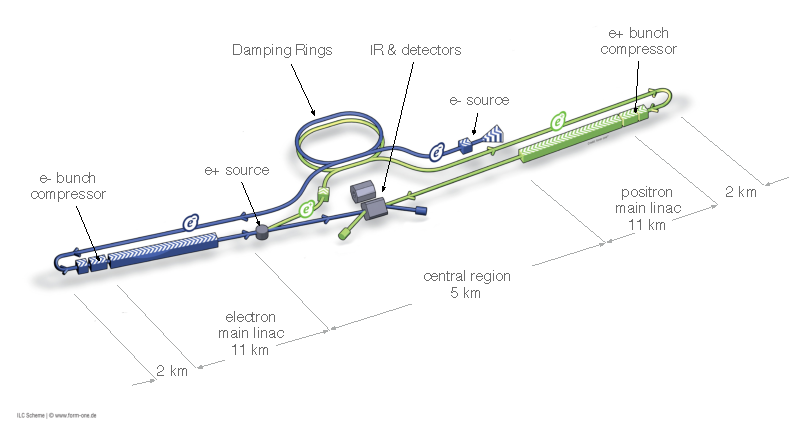
\includegraphics[scale=1.0]{./figures/ILC_schema.pdf}
      \caption{Sch\'ema de l'ILC.}
      \label{fig:ILC_schema}
    \end{center}
  \end{figure}
  
  Le d'injection comporte :
  
  \medskip
  
  \renewcommand{\labelitemi}{$\bullet$}
  
  \begin{itemize}
   
   \item une source d'\'electrons polaris\'es bas\'ee sur une photocathode DC,
   
   \item une source de positons polaris\'es, o\`u les positons sont obtenus \`a partir de paires d'\'electron-positon, elles-m\^emes obtenues gr\^ace aux photons de hautes \'energies produits par le passage du faisceau principal d'\'electron dans un ondulateur,
   
   \item deux anneaux de freinage \`a 5 GeV pour les \'electrons et positons d'une circonf\'erence de 3.5 $km$ et positionn\'es dans un tunnel commun,
   
   \item des syst\`emes de transports du faisceau entre les anneaux de freinage et les LINACs principaux, suivis d'un syst\`eme de compression (\`a deux \'etapes) du faisceau en paquets, avant injection.
   
   \end{itemize}
  
  \medskip
  
  Dans la version \`a 500 $GeV$, les deux LINACs principaux mesurent 11 $km$ de long et utilisent des cavit\'es supra-conductrices Radio Fr\'equence \`a 1.3 $GHz$ ce qui leur conf\`erent un gradient moyen d'acc\'el\'eration de 31.5 $MV/m$ (\`A l'\'echelle d'une cavit\'e des variations du champ acc\'el\'erateur de $\pm 20 \%$ sont attendues). Apr\`es avoir \'et\'e acc\'el\'er\'es dans les LINACs, les faisceaux d'\'electrons et de positons sont inject\'es dans deux syst\`emes oppos\'es d'une longueur de 2.2 $km$, conduisant les faisceaux jusqu'au point d'interaction. Les faisceaux se croisent alors avec un angle de 14 $mrad$ et la r\'egion d'interaction est recouverte par un d\'etecteur unique ou deux d\'etecteurs interchangeables. Cet angle de croisement permet d'obtenir une valeur de luminosit\'e optimale tout en facilitant l'extraction des faisceaux apr\`es leur croisement. Cette technique est sch\'ematis\'ee en figure \ref{fig:crab_crossing}
  
  \begin{figure}[!htb]
    \begin{center} 
      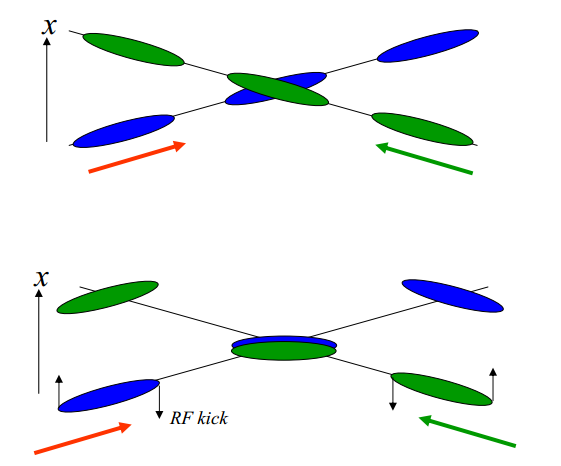
\includegraphics[scale=0.4]{./figures/crab_crossing.png}
      \caption{L'utilisation de cavit\'es de "Crab" permet d'incliner les paquets de particules afin qu'il se rencontrent face \`a face au point d'interaction. Cette technique permet de maximiser la luminosit\'e.}
      \label{fig:crab_crossing}
    \end{center}
  \end{figure}  
  
  \medskip
  
%   La r\'egion centrale visible en figure \ref{fig:ILC_schema_2} contient de nombreux sous-systèmes d'accélérations cl\'es. La source d'\'electrons, la source de positons (incluant la source auxiliaire de faible puissance), les anneaux de freinages des \'electrons et des positons sont situ\'es autour de la région d'interaction. Les anneaux de freinages sont d\'eplac\'es lat\'eralement pour éviter les perturbations avec les d\'etecteurs. Les sources d'électrons et de positons sont positionn\'ees dans le m\^eme tunnel que les syst\`emes conduisant les faisceaux au point d'interaction afin de r\'eduire les co\^uts et la taille de la région centrale. 

%   \begin{figure}[!htb]
%     \begin{center} 
%       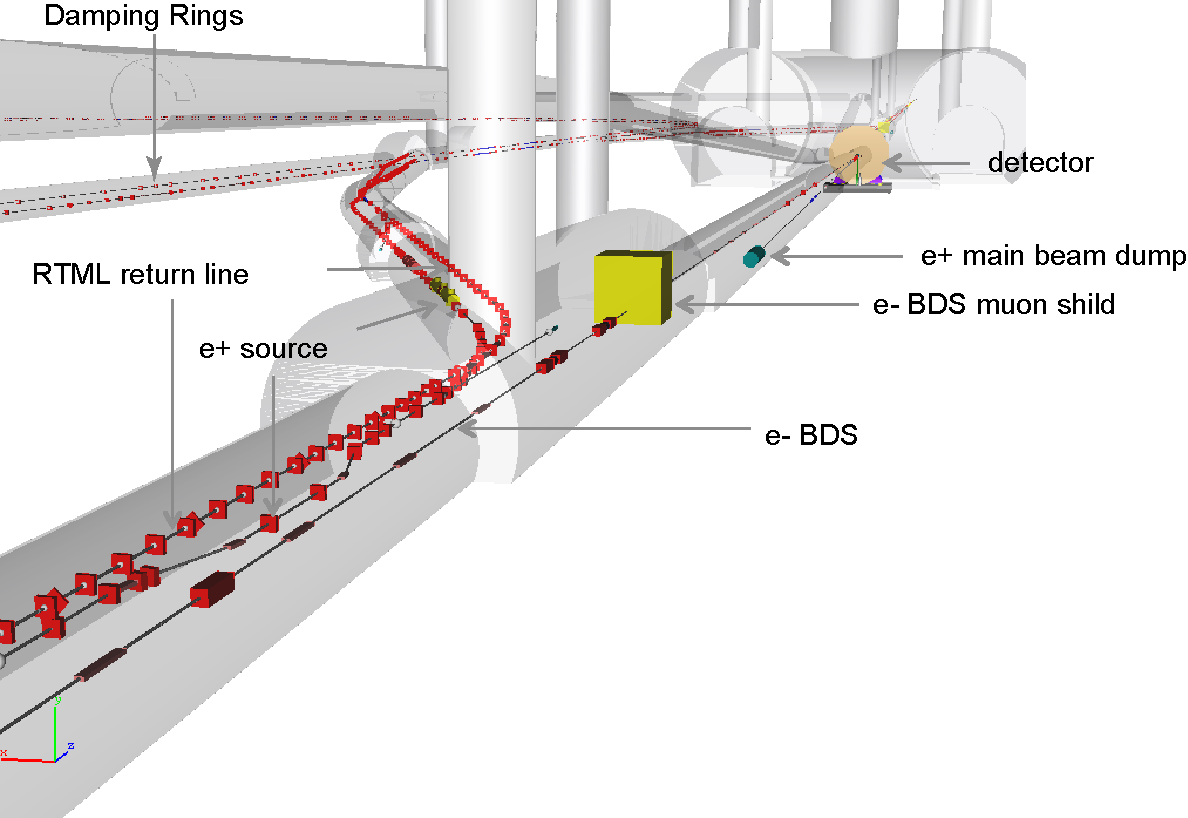
\includegraphics[scale=0.6]{./figures/ILC_region_centrale.pdf}
%       \caption{.}
%       \label{fig:ILC_schema_2}
%     \end{center}
%   \end{figure}
%   
%   \medskip
%   
%   Une \'etude g\'en\'erale de la physique \`a l'ILC men\'ee par un comit\'e de l'ICFA a conclu sur les principaux objectifs de physique qui devront être \'etudi\'es. Le GDE a alors établi les caract\'eristiques techniques principales de la machine \`a construire. 
  
  Les principales caract\'eristiques de la machine d\'erivant des objectifs de physique sont les suivants : 
  
  \medskip
  
  \renewcommand{\labelitemi}{$\bullet$}
  
  \begin{itemize}
   
   \item Une luminosit\'e qui doit conduire \`a $\int L dt = 500 \, fb^{-1}$ sur 4 ans,
   
   \item Une \'energie dans le centre de masse ajustable entre 200 et 500 $GeV$ (\'eventuellement option Giga-Z \`a 91 $GeV$ et Mega-W \`a 160 $GeV$),
   
   \item Une capacit\'e accrue \`a ajuster l'énergie dans le centre de masse entre 200 et 500 $GeV$,
   
   \item Une stabilit\'e de l'\'energie et une pr\'ecision sur celle-ci inf\'erieure \`a 0.1$\%$,
   
   \item Une polarisation des \'electrons $\geq 80 \%$.
   
   \end{itemize}
  
  \medskip  

%   De plus, le rapport de l'ICFA a identifi\'e diff\'erentes options qui devraient \^etre incluses dans la conception de la machine.
  
  De plus, il devra \^etre possible de mettre \`a jour la machine pour atteindre le $TeV$ dans le centre de masse. Un faisceau de positons polarisable est de plus souhaitable. Des caract\'eristiques plus d\'etaill\'ees de l'ILC sont list\'ees dans la table \ref{tab:paramILC}.
  
  \begin{table}[!htb]
  \begin{center}
  \begin{tabular}{|l|l|l|}  \hline
  Énergie max. dans le centre de masse & 500 & GeV  \\ \hline
  Pic de luminosit\'e & $\sim{2}\times10^{34}$ & $cm^{-2}s^{-1}$ \\ \hline
  Courant du faisceau & $9.0$ & mA \\ \hline
  Taux de r\'ep\'etition & $5$ & Hz \\ \hline
  Gradient moyen d'acc\'el\'eration & $31.5$ & MV/m \\ \hline
  Dur\'ee d'impulsion du faisceau & $0.95$ & ms \\ \hline
  Longueur totale du site & $31$ & km \\ \hline
  Puissance totale AC consomm\'ee & $\sim{230}$ & MW \\ \hline
  \end{tabular}
  \end{center}
  \caption{Principaux param\`etres du design de l'ILC \`a 500 $GeV$.}
  \label{tab:paramILC}
  \end{table}
  
%   L'ILC a \'et\'e con\c{c}u pour poss\'eder une \'energie réglable allant de 200 \`a 1000 $GeV$. Pour cela, les param\`etres de la machine ont \'et\'e optimis\'es en fonction du co\^ut, des risques et des performances de physiques. Le design cr\'e\'e est relativement conservatif et prend en compte certaines contraintes impos\'ees par les diff\'erents sous-syst\`emes d'acc\'el\'eration. Parmi celles-ci on peut lister des instabilit\'e de seuils (en particulier celle du nuage d'\'electrons dans l'anneau des positons), des \textit{temps de mont\'e} r\'ealistes pour les injecteurs et les extracteurs (kickers) et le désir de minimiser la circonf\'erence des anneaux.
  
  \medskip
  
  Pour r\'esumer l'ILC est un collisionneur d'\'electrons et de positons avec une \'energie r\'eglable entre 250 et 500 $GeV$ extensible \`a 1 $TeV$ dans le centre de masse. La technologie d'acc\'el\'eration radio-fr\'equence et la structure des faisceaux sont, de plus, adapt\'ees \`a la nature lin\'eaire du collisionneur. Apr\`es la description du complexe de l'acc\'el\'erateur, nous allons nous pencher sur les \'etudes physiques r\'ealisables \`a l'ILC. 
  
  %La production de positons dans l'ondulateur est d\'egrad\'e pour un faisceau d'électron d'énergie inf\'erieure \`a 150 $GeV$. Ainsi, pour des énergies dans le centre de masse inf\'erieures \`a 300 $GeV$ (faisceau d'électrons inf\'erieur \`a 150 $GeV$) le taux de r\'ep\'etition est augment\'e \`a 10 $Hz$. \\ la suite -> ?????? \\
  
  %La dur\'ee maximale de la pulsation du faisceau est contrainte \`a $\approx$ 1.6 $msec$.Il s'agit de ce qu'il est possible d'atteindre avec les klystrons multi-faisceaux \footnote{Les Klystrons convertissent et amplifient des faisceaux d'\'electrons en ondes radio-fr\'equence} (1.3 $GHz$ et 10 $MW$) et les modulateurs actuels. Le courant du faisceau est limit\'e par le nombre de klystrons (pic de puissance) et les modes d'ordre plus \'elev\'e.
    
  \subsection{Programme de physique}
  \label{sect:prog_physique}

%   Le mod\`ele standard de la physique des particules et de leurs interactions a pass\'e de nombreux tests de validation de la part de certains physiciens exp\'erimentateurs \cite{ALEPH:2010aa}. Le mod\`ele standard contient un m\'ecanisme de brisure de la symétrie \'electrofaible responsable de la masse des particules. Ce m\'ecanisme est appel\'e m\'ecanisme de Higgs et son boson vecteur, le boson de Higgs. Un candidat au boson de Higgs \'et\'e d\'ecouvert au LHC. Avec la faible pr\'ecision obtenue sur ses paramètres (masse, largeur, spin, couplages) \`a ce jour,  ce candidat est conforme au pr\'edictions du mod\`ele standard. Pour compl\'eter l'\'etude du mod\`ele standard et pour tenter de le d\'epasser, il faut mesurer avec pr\'ecision les propri\'et\'es de ces constituants et en particulier, le boson de Higgs. Cependant le mod\`ele standard n'explique pas plusieurs faits exp\'erimentaux importants et plusieurs questions restent encore en suspens :
% 
%   \medskip
% 
%   \renewcommand{\labelitemi}{$\bullet$}
% 
%   \begin{itemize}
%    \item La particule d\'ecouverte au LHC explique-t-elle enti\`erement l'origine de la brisure de la symétrie \'electro-faible et la masse des particules \'el\'ementaires ?
%    \item Pourquoi la particule d\'ecouverte au LHC a-t-elle cette masse et non une masse plus importante ? Ce probl\`eme est connu sous le nom de probl\`eme de hi\'erarchie.
%    \item Quelle est l'origine de la mati\`ere noire ?
%    \item Pourquoi l'univers est-il compos\'e de plus de mati\`ere que d'antimati\`ere ?
%    \end{itemize}
% 
%    \medskip

%    L'ILC permettra de chercher des r\'eponses \`a toutes ces questions.
   Comme nous l'avons d\'ej\`a vu, en juillet 2012, les collaborations ATLAS et CMS ont annonc\'e la d\'ecouverte d'une particule d'une masse de 125 $GeV/c^2$ compatible avec le boson de Higgs standard\cite{Aad:2012tfa, Chatrchyan:2012ufa}. Ces exp\'eriences du LHC continuent de raffiner leurs mesures sur les propri\'et\'es de cette nouvelle particule. Cependant, la pr\'ecision de ces mesures sera limit\'ee par la nature hadronique du collisionneur. De plus, les questions sur la physique au del\`a du mod\`ele standard restent encore en suspens et l'ILC sera le compl\'ement id\'eal au LHC pour tenter de r\'epondre \`a ces questions. Dans cette section nous allons d\'ecrire le programme de physique de l'ILC tel qu'il est d\'ecrit dans le \textit{TDR} \cite{Baer:2013cma}. Nous ferons ainsi une revue non exhaustive des mesures les plus importantes r\'ealisables \`a l'ILC.
   
   \medskip
   
   L'ILC \'etant un acc\'el\'erateur lin\'eaire, son \'energie dans le centre de masse est r\'eglable. Ainsi, diff\'erents programmes exp\'erimentaux pourront avoir lieu \`a l'ILC en fonction de l'\'energie disponible dans le centre de masse. Les diff\'erents programmes envisag\'es sont les suivants :
   
   \paragraph{91 GeV et 160 GeV :} \`A l'\'energie de 91 GeV on atteint la r\'esonance du boson $Z$ et \`a environ 160 GeV, on atteint le seuil pour de production de paires $W^+ W^-$ : $e^+ e^- \rightarrow W^+ W^-$. Comme l'ILC poss\'edera une luminosit\'e d'environ deux \`a trois ordre de grandeur au dessus de celle du LEP, cela permettra de mettre en place un programme \textit{GigaZ} et un programme \textit{MegaW}. L'objectif du programme \textit{GigaZ} est la mesure de l'asym\'etrie droite/gauche du Z et la mesure des couplages au Z avec une pr\'ecision d'un ordre de grandeur sup\'erieure compar\'ee \`a celle obtenue par le LEP. Le programme \textit{MegaW} vise quant \`a lui la mesure de la masse du W avec une pr\'ecision atteignant le $MeV/c^2$.
   
   \paragraph{250 GeV :} Cette \'energie correspond au pic de la section efficace du \textit{Higgstrahlung}. Ce dernier \'etant le nom donn\'e \`a la production de Higgs selon la r\'eaction $e^+ e^- \rightarrow Z h$. Avec $h$ le boson de Higgs de masse 125 $GeV/c^2$ d\'ecouvert au LHC. Que ce boson soit le boson de Higgs standard ou un autre boson, l'\'etude des couplages et des nombres quantiques de cette particule devrait \^etre r\'ealis\'ee avec pr\'ecision. La m\'ethode de la masse de recul devrait permettre une reconstruction de la masse de ce boson ind\'ependamment de toutes hypoth\`eses sur les produits de d\'esint\'egration du Higgs. (La masse manquante et les modes de d\'esint\'egration inattendus \'etant pris en compte). Nous reviendrons sur cette m\'ethode un peu plus loin.
   
   \paragraph{350-400 GeV :} Le seuil de production de paires $t\overline{t}$ apparaît aux alentour de 350 $GeV$. A cause de son très faible temps de vie, le quark top et son anti-particule ne poss\`edent pas d'\'etat li\'e (pas de particule compos\'ee de quark ou d'anti-quark top). Cependant, la section efficace de production de paires $t\overline{t}$ exhibe une forme particuli\`ere pr\`es du seuil de production. Cette forme est tr\`es pr\'ecis\'ement pr\'edite par des calculs de QCD perturbative. Un balayage en \'energie autour du seuil devrait permettre de reconstituer cette forme. La masse du quark top pourra alors \^etre mesur\'ee avec une pr\'ecision d'environ 100 $MeV/c^2$. La mesure pr\'ecise des \'etats finals au seuil de production et aux \'energies plus hautes livreront des mesures de pr\'ecision contraignant la brisure de la symétrie \'electrofaible. Au alentour de cette \'energie la section efficace de production de Higgs par fusion $WW$ devient importante. La mesure de la r\'eaction $e^+ e^- \rightarrow \nu \nu h$ devrait fournir une mesure pr\'ecise du couplage $hWW$. En effet, la section efficace de ce processus augmente avec l'\'energie dans le centre de masse (voir figure \ref{fig:energyHiggs}). Cette production de boson de Higgs offrira une statistique \'elev\'ee pour l'\'etude des d\'esint\'egrations rares du boson de Higgs. De plus une mesure fine des couplages au W \`a l'aide de la r\'eaction $e^+ e^- \rightarrow W^+ W^-$ permettra l'\'etude d'une d\'eviation de ces couplages par rapport au mod\`ele standard.
   
  \begin{table}[htb!] 
  \footnotesize{
  \begin{center}
  \begin{tabular}{rccc}
  \'Energie             &   R\'eaction  &  Objectif physique     
  \\  \hline \hline
  91~GeV            &       $e^+e^-  \to Z$     &      
   mesures ultra-pr\'ecises du mod\`ele \'electrofaible        \\   \hline
  160~GeV            &       $e^+e^-  \to WW$     &
  mesure ultra-pr\'ecise de la masse du $W$         \\   \hline
  250~GeV         &    $e^+e^-  \to Z h$     &      mesures pr\'ecises des couplages au Higgs           \\ 
			    \hline
  350--400~GeV         &      $e^+e^-  \to t\bar t$        &  
    mesures de la masse du quark top et de ses couplages                \\
    &    $ e^+e^-  \to WW$     &     mesures pr\'ecises des couplages au $W$             \\ 
			&     $ e^+e^-  \to \nu\bar\nu h $   & 
  mesures pr\'ecises des couplages au Higgs     \\   \hline
  500~GeV         &      $e^+e^-  \to f\bar f   $       &   
  recherche précise du $Z'$      \\ 
      &  $ e^+e^-  \to t\bar t h$    &      mesures des couplages Higgs-top      \\
			  &      $e^+e^-  \to Z h h $       &     mesure de l'auto-couplage du Higgs            \\
			&   $   e^+e^- \to  \tilde \chi \tilde \chi$  &
			recherche de la supersym\'etrie   \\  
			&    $  e^+e^- \to AH, H^+H^-  $  &
			recherche d'\'etats \'etendus du Higgs   \\  \hline
  700--1000~GeV &        $ e^+e^-  \to \nu\bar \nu hh $ & 
	  mesures des autocouplages du Higgs     \\ 
			    &    $e^+e^-  \to \nu\bar \nu VV$ &  recherche d'un Higgs composite  \\ 
			    &    $e^+e^-  \to \nu\bar \nu t\bar t$ &
			    recherche de Higgs et top composites  \\
			    &    $e^+e^-  \to \tilde t \tilde{ t}^* $ &
			  recherche de la supersym\'etrie  \\
			    \hline
  \end{tabular}
  \end{center} }
  \caption{Principaux processus physiques \'etudi\'es \`a l'ILC pour diff\'erentes \'energies dans le centre de masse. Le tableau indique les diff\'erentes réactions du mod\`ele standard accessibles en fonction de l'augmentation en \'energie, ainsi que les principaux objectifs physiques. Une r\'eaction list\'ee \`a une \'energie donn\'ee sera aussi \'etudi\'ee pour toutes les \'energies plus \'elev\'ees.}
  \label{tab:ILCprogramX}
  \end{table}
   
   \paragraph{500 GeV :} A cette \'energie l'ILC fonctionnera \`a son \'energie et \`a sa luminosit\'e nominale. Les donn\'ees collect\'ees permettront alors d'am\'eliorer les pr\'ecisions sur les mesures des processus sus-mentionn\'es. A cette \'energie, l'\'etude des r\'eactions $e^+ e^- \rightarrow f \overline{f}$ ou $f$ peut \^etre un quark ou un lepton, offre la possibilit\'e d'\'etudier la physique au delà du mod\`ele standard. Du fait de leur simplicit\'e, les \'etats finals de ces processus sont facilement distinguables exp\'erimentalement. De plus, les calculs perturbatifs correspondant, bas\'es sur le mod\`ele standard, ont d\'ejà \'et\'e r\'ealisés et donnent des r\'esultats tr\`es pr\'ecis. De faibles d\'eviations sur les pr\'edictions du mod\`ele standard pourraient permettre d'explorer une nouvelle physique \`a des \'echelles d'\'energie bien sup\'erieure \`a celle du centre de masse. L'existence du boson $Z'$, la nature composite des fermions ou encore certains mod\`eles \`a dimensions suppl\'ementaires pourront \^etre test\'es. Le d\'etecteur de vertex jouera un r\^ole primordial dans l'identification des saveurs mises en jeu. De plus, de nouvelles particules pourront \^etre recherch\'ees comme certaines particules supersym\'etriques ou comme d'autres \'etats d'un secteur de Higgs composite. De plus, \`a cette \'energie l'\'etude du couplage du quark top au Higgs devient possible.
%    Cette recherche de nouvelles particules est tr\`es difficile au LHC pour certaines gammes de param\`etres.
   
   \paragraph{1 TeV :} \`A cette \'energie de fonctionnement, envisag\'ee apr\`es une mise \`a jour de l'ILC, de nombreuses nouvelles mesures seront possibles. Ces mesures permettront entre autre d'explorer : le couplage du Higgs au quark top, les auto-couplages du Higgs et les mod\`eles de Higgs composite. De nouvelles particules exotiques pourront de plus \^etre recherch\'ees. Les donn\'ees produites permettront aussi d'am\'eliorer la pr\'ecision des mesures d\'ej\`a r\'ealis\'ees \`a des \'energies dans le centre de masses inf\'erieures.
   
% Le quark top est le plus massif des six quarks que nous connaissons. Sa grande masse, comparable à celle d'un atome d'or, lui confère une caractéristique particulière dans la famille des quarks : il n'existe pas d'état lié (donc de particule) avec un quark top (ou antitop). C'est en détectant ses produits de désintégration que l'on mesure les caractéristiques de ce quark.

  \medskip

  Le tableau \ref{tab:ILCprogramX} r\'esume tous ces programmes. Apr\`es avoir r\'ealis\'e une revue des \'etudes possibles \`a l'ILC nous allons nous pencher plus particuli\`erement sur la physique du Higgs, du top et la supersym\'etrie \`a l'ILC.

   \subsubsection{Physique du Higgs}
  
   La premi\`ere phase du programme de recherche sur le Higgs sera constitu\'ee par la mesure pr\'ecise des propri\'et\'es du boson de Higgs d\'ecouvert au LHC. L'objectif sera de savoir si ce boson est vraiment compatible avec le mod\`ele standard ou si des diff\'erences apparaissent.
  
  \medskip

   La premi\`ere \'etape de notre cheminement consiste \`a savoir quels sont les modes de production de Higgs du mod\`ele standard observables \`a L'ILC. Pour cela nous allons discuter les sections efficaces de production du Higgs standard \`a l'ILC. La figure \ref{fig:feynmanHiggs2} repr\'esente les diagrammes de \textit{Feynman} des trois processus majoritaires de production du Higgs \`a l'ILC.
   
  \begin{figure}[!htb]
    \begin{center} 
      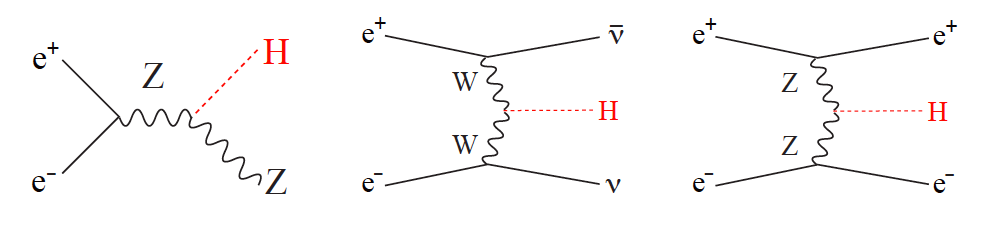
\includegraphics[scale=0.40]{./figures/feynman_Higgs.png}
      \caption{Diagrammes de \textit{Feynman} pour les 3 processus majeurs de production de Higgs \`a l'ILC : $e^+ e^- \rightarrow Z h$ (\`a gauche), $e^+ e^- \rightarrow \nu \overline{\nu} h$ (au centre), et $e^+ e^- \rightarrow e^+ e^- h$ (\`a droite). }
      \label{fig:feynmanHiggs2}
    \end{center}
  \end{figure}
   
  \begin{figure}[!htb]
    \begin{center} 
      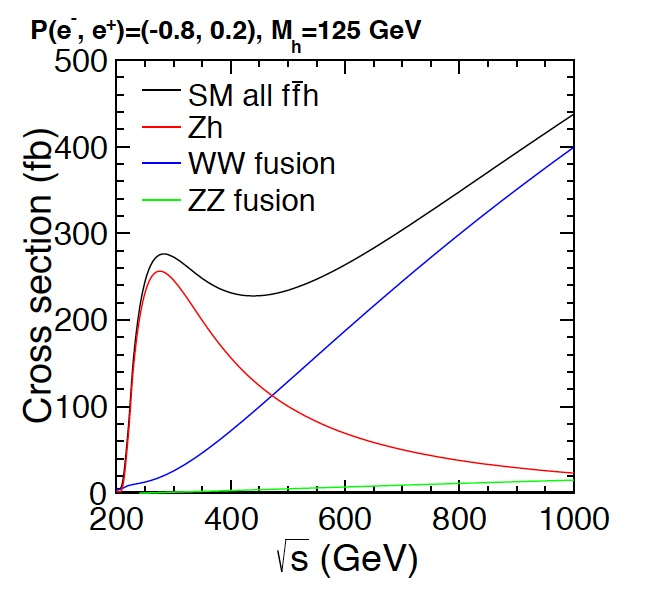
\includegraphics[scale=0.40]{./figures/energy_Higgs.jpg}
      \caption{Section efficace de production pour le Higgstrahlung ($e^+ e^- \rightarrow Z h$), la fusion WW ($e^+ e^- \rightarrow \nu \overline{\nu} h$) et la fusion ZZ ($e^+ e^- \rightarrow e^+ e^- h$) en fonction de l'\'energie dans le centre de masse, pour une masse du Higgs de 125 $GeV$, et pour une polarisation de faisceau ($P_{e^-}$, $P_{e^+}$) = ($-0.8$, $+0.2$). }
     \label{fig:energyHiggs}
     \end{center}
  \end{figure}
   
   D'autres processus existent, cependant ils ont une section efficace d'au moins un ordre de grandeur inf\'erieur \`a la fusion $ZZ$ et n'apparaissent qu'\`a partir de 350-500 $GeV$ dans le centre de masse (voir figure \ref{fig:crossSectionHiggs}). En figure \ref{fig:energyHiggs} est illustr\'ee la section efficace de production des trois processus majoritaires en fonction de l'\'energie dans le centre de masse, obtenue pour une polarisation de faisceau $(Pe^- , Pe^+ ) = (-0.8 , +0.2)$. La section efficace maximale de la r\'eaction $e^+ e^- \rightarrow Zh$ est obtenue aux alentours de 250 GeV dans le centre de masse. Elle vaut environ 220 $fb$. Cette r\'eaction porte le nom de Higgstrahlung. \`A cette \'energie la fusion $W^+W^-$ ($e^+ e^- \rightarrow \nu \overline{\nu} h$) poss\`ede une section efficace un ordre de grandeur au dessous. Cependant, alors que le Higgstrahlung diminue avec l'augmentation de l'\'energie disponible dans le centre de masse \`a partir de 250 GeV, la fusion $WW$ augmente avec la hausse en \'energie. Ainsi aux alentours de 500 GeV le Higgstrahlung et la fusion $WW$ ont environ la même section efficace (environ 120 $fb$). A plus haute \'energie, la section efficace de fusion $WW$ augmente encore et le Higgstrahlung d\'ecro\^it. Ainsi avec l'\'energie maximale de 1 $TeV$ atteignable \`a l'ILC, la section efficace de fusion $WW$ vaut environ 400 $fb$ et celle du Higgstrahlung 20 $fb$. La fusion $ZZ$ est quant \`a elle minoritaire. Elle passe d'environ quelques $fb$ \`a 250 GeV \`a 20 $fb$ \`a 1 $TeV$. Ainsi, plusieurs programmes de physique selon que l'on soit \`a une \'energie de 250, 500 ou 1000 $GeV$ dans le centre de masse sont r\'ealisables. 
   
   \medskip
   
   \begin{figure}[!htb]
     \begin{center} 
       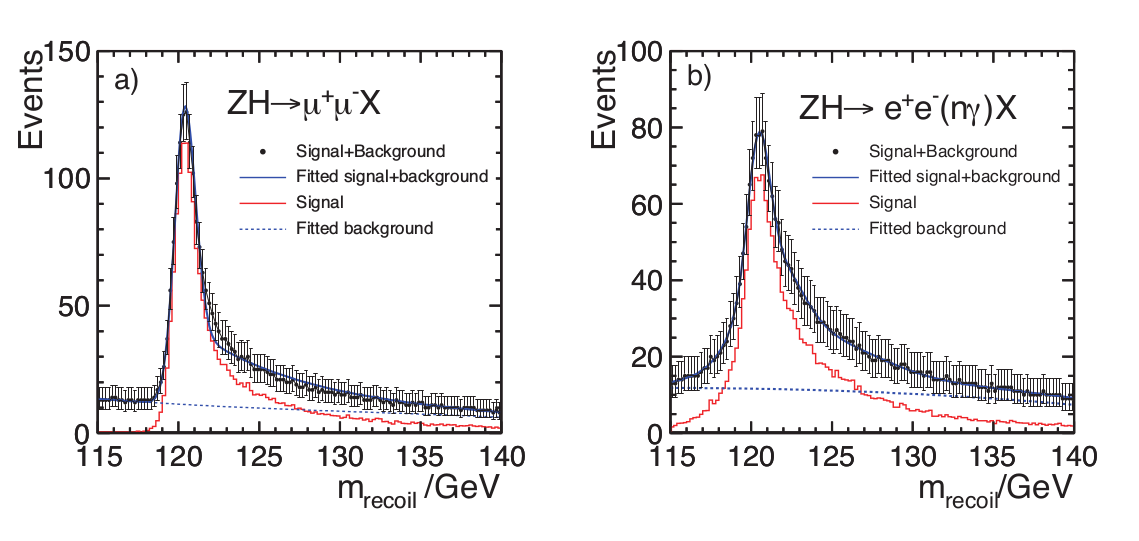
\includegraphics[scale=0.35]{./figures/recoil_mass_Higgs.png}
       \caption{ R\'esultats d'une simulation de 250 $fb^{-1}$ du Higgsstrahlung $e^+ e^- \rightarrow Z h$ avec \`a gauche $Z \rightarrow \mu^+ \mu^-$  et \`a droite $Z \rightarrow e^+ e^- (+n \gamma)$ comme attendu dans le d\'etecteur ILD de l'ILC. Ces r\'esultats sont montr\'es pour une polarisation $P(e^+ , e^-) = (+0.3 , -0.8)$ (TDR Volume Physics \cite{Behnke:2013lya} p288)}
     \label{fig:simuILC}
     \end{center}
  \end{figure}

% TDR page 288
  
   Le programme de l'ILC devrait donc commencer par l'exploitation du pic du Higgsstrahlung vers 250 $GeV$. Pour cela, la masse du Higgs sera reconstruite grâce \`a sa masse de recul $M_H$. L'int\'er\^et de cette m\'ethode repose sur le fait que la masse calcul\'ee est ind\'ependante de toute hypoth\`ese sur les produits de d\'esint\'egration du Higgs. Celui-ci peut alors se d\'esint\'egrer en invisible ou en particules exotiques sans que cela influe sur la mesure de sa masse. La masse de recul du Higgs est calcul\'ee selon la relation suivante :
   
   \begin{equation}
    M_H^2 = s + M_Z^2 - 2 \sqrt{s}(E_1 + E_2)
   \end{equation}
 
   o\`u $M_H$ est la masse de recul du boson de Higgs, $M_Z$ la masse du boson $Z$ et $E1$ et $E2$ sont les \'energies des produits de d\'esint\'egration du $Z$. La figure \ref{fig:simuILC} repr\'esente la simulation bas\'ee sur 250 $fb^{-1}$ de donn\'ees, de la masse de recul du Higgs dans le cas ou le Z se d\'esint\`egre en une paire de muons $\mu^+ \mu^-$ (ou $e^+ e^-$). La m\'ethode de la masse de recul comme illustr\'ee en figure \ref{fig:simuILC} permet d'obtenir une pr\'ecision statistique de l'ordre de 40 $MeV$ sur la masse de recul du Higgs pour le canal $Z \rightarrow \mu^+ \mu^-$ avec une \'energie de 250 $GeV$ dans le centre de masse et 250 $fb^{-1}$ de donn\'ees simul\'ees. Une pr\'ecision de l'ordre de 80 $MeV$ est obtenue dans les m\^emes conditions de simulation pour le canal $Z \rightarrow e^+ e^-$. La combinaison des deux r\'esultats donne une pr\'ecision sur la mesure d'environ 32 $MeV$ \cite{Abe:2010aa} \cite{Li:2012taa}.
   
   \medskip
   
   \begin{figure}[!htb]
     \begin{center} 
       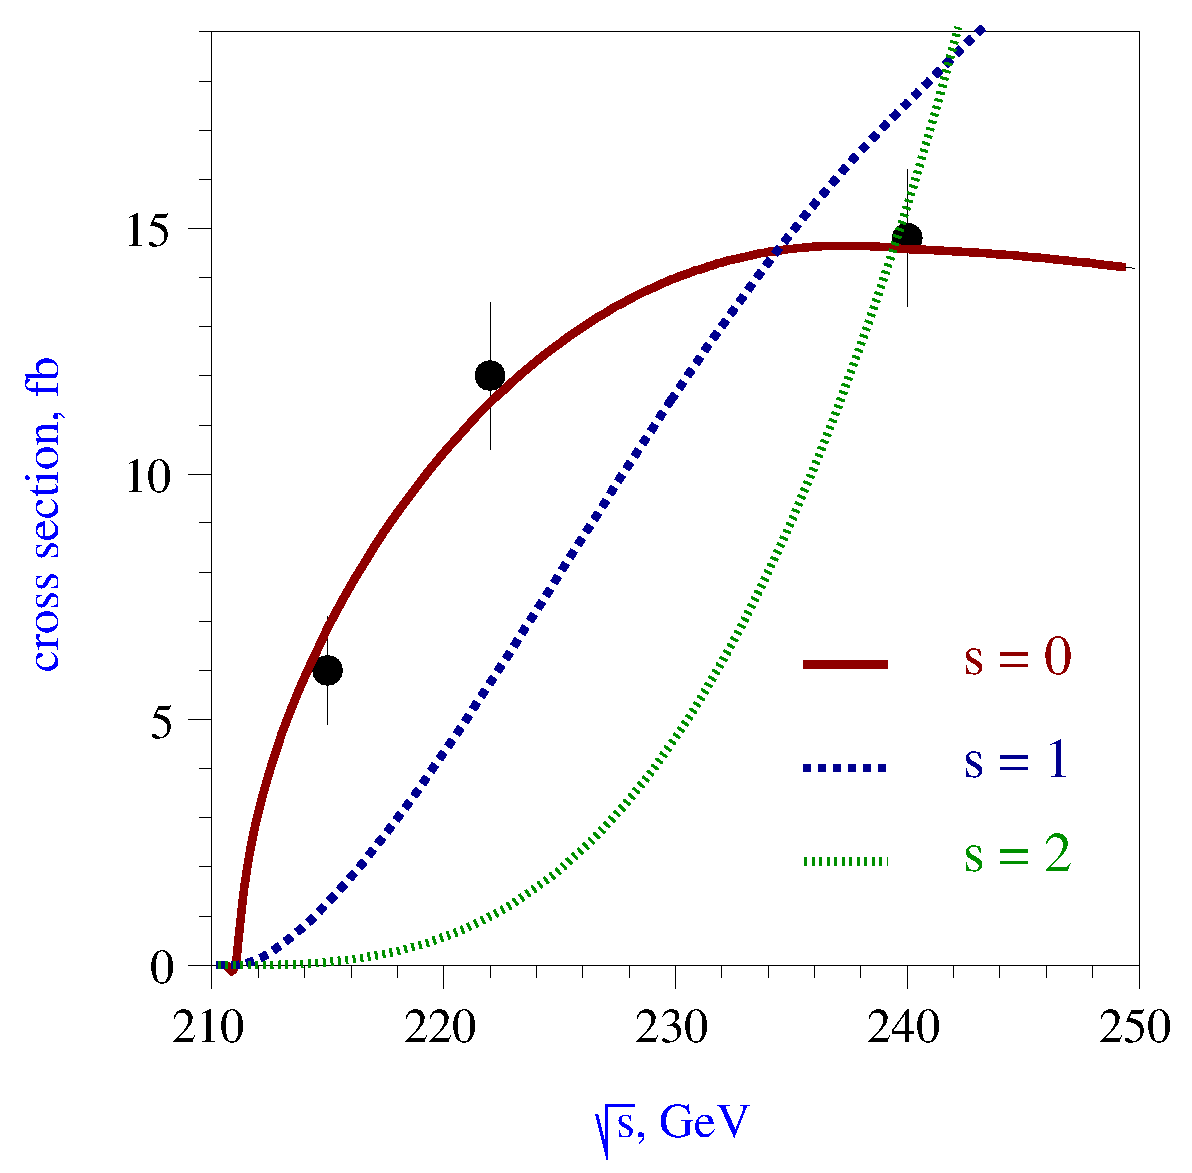
\includegraphics[scale=0.35]{./figures/higgs_spin1.eps}
       \caption{ Comportement de la section efficace $e^+ e^- \rightarrow Zh$ au seuil de production, en fonction du spin et de la valeur de CP. Les trois courbes indiquent le comportement th\'eorique de la section efficace au seuil de production pour $J^P$ = $0^+$ , $1^-$, et $ 2^+$. 3 points de mesures avec 20 $fb^{-1}$ de donn\'ees permettent de distinguer les diff\'erentes possibilit\'es. \cite{Dova:2003py} }
     \label{fig:spinHiggs}
     \end{center}
   \end{figure}
   
   Le programme de mesure \`a 250 $GeV$ inclura la mesure de la masse mais aussi du spin et de CP pour le boson de Higgs. Ainsi, l'ILC procurera un test complémentaire au LHC pour la mesure du spin du boson de Higgs. La m\'ethode de mesure est bas\'ee sur le comportement au seuil de production pour la section efficace du Higgstrahlung $e^+ e^- \rightarrow Zh$. Cette section efficace ne varie pas de la m\^eme mani\`ere selon les valeurs du spin et de CP pour le boson de Higgs. La possibilit\'e d'un spin 1 a \'et\'e exclue par l'observation du canal $h\rightarrow \gamma \gamma$ au LHC. Pour un boson de Higgs de spin 0, le comportement au seuil de la section efficace $e^+ e^- \rightarrow Zh$ \`a l'ILC varie comme lin\'eairement pour une valeur de CP paire et comme $x^3$ pour une valeur de CP impaire (voir figure \ref{fig:spinHiggs} \cite{Dova:2003py}). Pour un boson de Higgs de spin 2, la section efficace au seuil augmente comme $x^3$. Pour des spins plus \'elev\'es, la section efficace au seuil augmentera selon des puissances de $x^n$ plus grande que 3. Des mesures de la section efficace juste au dessus du seuil de production devraient permettre de trancher entre toutes ces possibilit\'es. Trois points de mesure nécessitant 20 $fb^{-1}$ de donn\'ees permettront de s\'eparer toutes les possibilit\'es et donc d'obtenir le spin et la valeur de CP \cite{Dova:2003py}.   
   
   \medskip
% Cette voie de d\'esint\'egration impose une valeur positive pour la conjugaison de charge.


   \begin{figure}[!htb]
   \renewcommand{\figurename}{Table}
   \begin{center} 
      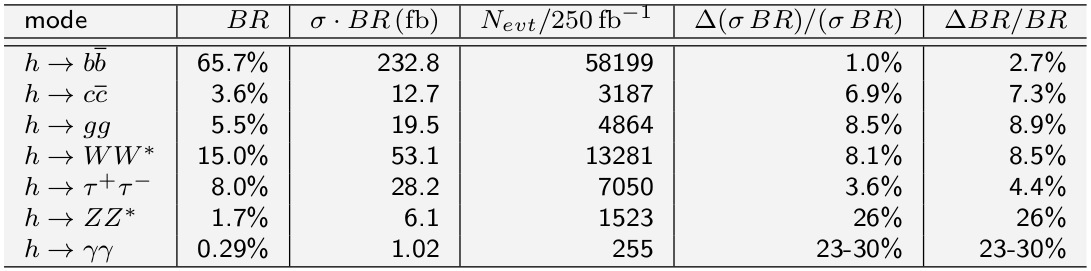
\includegraphics[scale=0.38]{./figures/table_BR_Higgs_MS.png}
      \caption{ Pr\'ecision sur les rapports de branchement pour un Higgs standard \`a 120 $GeV/c^2$, obtenue avec une simulation compl\`ete du d\'etecteur, pour une \'energie dans le centre de masse de 250 $GeV$ et une luminosit\'e int\'egr\'ee $L = 250 \, fb^{-1}$ et une polarisation des faisceaux $(e^- , e^+ ) = (-0.8, +0.3)$. Les erreurs sur les rapports de branchements incluent des erreurs de $2.5 \%$ sur $\sigma$. \cite{Ono:2013sea}}
     \label{fig:BR_SM_Higgs}
     \end{center}
  \end{figure}
  
   Les taux de d\'esint\'egration du boson de Higgs pourront \^etre mesur\'es avec pr\'ecision. Le tableau \ref{fig:BR_SM_Higgs} indique les rapports de branchement pour les diff\'erents modes de d\'esint\'egration pour le Higgs du mod\`ele standard. Les mesures qui seront r\'ealis\'ees \`a l'ILC, incluront  les d\'esint\'egrations invisibles ou les \'etats finaux inhabituels. Compar\'e au LHC o\`u de tels \'ev\`enements sont tr\`es difficilement s\'eparables du bruit de fond du mod\`ele standard, l'ILC permettra ces mesures avec une grande pr\'ecision. Dans le mod\`ele standard, les couplages du Higgs aux fermions sont proportionnels \`a la masse des fermions :
   
   \begin{equation}
    g_{hf\overline{f}} = \cfrac{m_f}{v}
   \end{equation}
  
    Et les couplages du Higgs aux bosons de jauge sont proportionnels \`a la masse au carr\'e de ces bosons. Avec $V = W , Z$, on a : 
    
    \begin{equation}
     g_{hVV} = \cfrac{2 m_V^2}{v}
    \end{equation}

%    \begin{figure}[!htb]
%      \begin{center} 
%        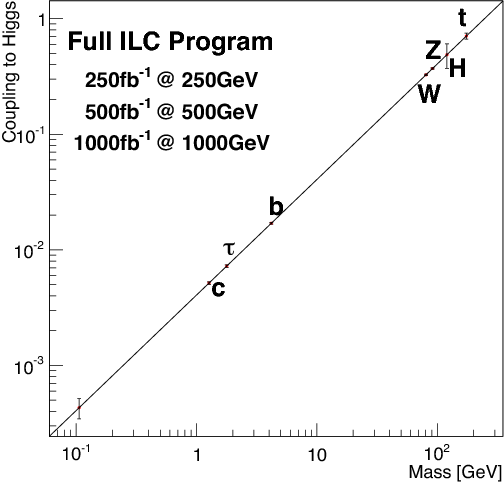
\includegraphics[scale=0.50]{./figures/Chapter_Theory_figs_mass-coupling1TeV.png}
%        \caption{ Les pr\'edictions des mesures des couplages au Higgs \`a l'ILC sont indiqu\'ees sur cette figure. La quantit\'e de donn\'ees utilis\'ee prend en compte l'ensemble des programmes envisag\'ees \`a l'ILC y compris celui \`a 1 $TeV$. }
%      \label{fig:HiggsCoupling}
%      \end{center}
%    \end{figure}
 
   Ainsi, des mesures de grande pr\'ecision des taux de d\'esint\'egration du boson de Higgs selon diff\'erentes voies (quarks, leptons et bosons) permettront de savoir si seul le champ de Higgs conf\`ere leur masse aux particules \'el\'ementaires ou si d'autres particules partagent le rôle de g\'en\'erateur de la masse. Il existe en effet plusieurs sc\'enarios de nouvelle physique qui g\'en\`erent des d\'eviations sur ces valeurs inf\'erieures \`a 10$\%$ par rapport au mod\`ele standard \cite{Gupta:2013}. On attirera l'attention du lecteur sur les voies de d\'esint\'egration $h \rightarrow b\overline{b}$ et $h \rightarrow c\overline{c}$ repr\'esentant respectivement environ $65.7\%$ et $3.6\%$ des d\'esint\'egrations du Higgs standard. Nous focaliseront aussi l'attention sur le canal $\tau^- \tau^+$ repr\'esentant environ $8\%$ de ces d\'esint\'egrations. Toutes ces saveurs devront \^etre reconstruites gr\^ace au d\'etecteur de vertex. 
   
   \medskip
   
   La largeur du boson de Higgs du mod\`ele standard \'etant estim\'ee \`a environ 4 $MeV/c^2$, une mesure directe aussi pr\'ecise ne pourra pas \^etre effectu\'ee \`a l'ILC. Cependant, la section efficace du processus $e^+ e^- \rightarrow Zh$ est proportionnelle au couplage $g_{hZZ}$ au carr\'e. Comme la largeur du processus de d\'esint\'egration $h \rightarrow ZZ^*$, $\Gamma(h \rightarrow ZZ^*)$, est proportionnelle \`a la constante de couplage $g_{hZZ}$ au carr\'e, la section efficace $e^+ e^- \rightarrow Zh$ est aussi proportionnelle \`a la largeur $\Gamma(h \rightarrow ZZ^*)$ \cite{Durig:2014lfa}. Cette derni\`ere largeur peut donc \^etre calcul\'ee \`a partir de la mesure pr\'ecise de la section efficace du processus $e^+ e^- \rightarrow Zh$. Étant donn\'e le rapport de branchement $BR(h \rightarrow ZZ^*)$ obtenu gr\^ace \`a la m\'ethode de la masse de recul, la largeur du boson de Higgs est donn\'ee par : 
   
   \begin{equation}
    \Gamma_{tot} = \dfrac{\Gamma(h \rightarrow ZZ^*)}{BR(h \rightarrow ZZ^*)}
   \end{equation}
 
   Le rapport de branchement $BR(h \rightarrow ZZ^*)$ \'etant faible ($\approx 1.7 \%$), une statistique importante est n\'ecessaire afin d'obtenir une mesure pr\'ecise. \`A 250 GeV avec 250 $fb^{-1}$ de donn\'ees collect\'ees, une pr\'ecision d'environ 26\% est attendue pour $BR(h \rightarrow ZZ^*)$. Afin d'augmenter la pr\'ecision sur la mesure de la largeur du Higgs l'utilisation du mode de d\'esint\'egration $h \rightarrow WW^*$ peut aussi \^etre utilis\'e. Une pr\'ecision sur la largeur du Higgs d'environ 2$\%$ pourra \^etre atteinte avec 250 $fb^{-1}$ de donn\'ees \`a 250 $GeV$ plus 500 $fb^{-1}$ de donn\'ees \`a 500 $GeV$.

   \medskip
   
   Dans la région d'\'energie 350-400 $GeV$ dans le centre de masse et plus haut, la r\'eaction $e^+ e^- \rightarrow WW$ permettra de sonder le mod\`ele standard \`a haute \'energie. Au fur et \`a mesure que l'\'energie monte, le processus de fusion $WW$ ($e^+ e^- \rightarrow \nu \overline{\nu} h$) cro\^it et une mesure plus pr\'ecise du couplage $hWW$ est alors possible. Il s'agit d'une des valeurs cruciales dans l'\'etude pr\'ecise du boson de Higgs.
   
   \medskip
  
  \begin{figure}[!htb]
    \begin{center} 
      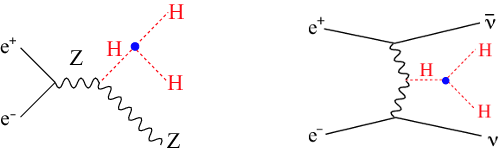
\includegraphics[scale=0.60]{./figures/tripleH_diagram.png}
      \caption{Diagrammes de \textit{Feynman} des processus $e^+ e^- \rightarrow Zhh$ et $e^+  e^- \rightarrow \nu_e \overline{\nu_e} hh$. Triple auto-couplage du Higgs.}
     \label{fig:triple-self_couplingHiggs}
     \end{center}
  \end{figure}    

   \`A 500 $GeV$ dans le centre de masse, deux processus importants \`a la compr\'ehension de la brisure de la sym\'etrie \'electrofaible deviennent accessibles \`a la mesure, le couplage de Yukawa du quark top et le terme d'auto-couplage triple du Higgs. La mesure du couplage de Yukawa du quark top sera accessible \`a partir de la r\'eaction $e^+ e^- \rightarrow t \overline{t} h$. La mesure de ce couplage permettra de mieux comprendre le m\'ecanisme de la g\'en\'eration des masses des fermions. 
   
   Une pr\'ecision de $\Delta g_t /g_t \approx 10\%$ sera possible avec une reconstruction du signal $e^+ e^- \rightarrow ttH$ en 6-jets + lepton et 8-jets, avec un Higgs \`a 120 GeV, une polarisation des faisceaux $(Pe^- , Pe^+ ) = (-0.8, +0.3)$ , et une luminosit\'e int\'egr\'ee de 1 $ab^-{1}$ \cite{Yonamine:2011jg}.

%    le canal $e^+ e^- \rightarrow ttH \rightarrow bW^- bW^+ b\overline{b}$ pour 1 $ab^{-1}$ de luminosit\'e int\'egr\'ee \`a 500 $GeV$ et pour un boson de Higgs de 120 GeV \cite{Tabassam:2012it}. Une pr\'ecision de $\Delta g_t /g_t \approx 28\%$ sera possible avec le canal $e^+ e^- \rightarrow ttH \rightarrow bW^- bW^+ b\overline{b}$ pour 1 $ab^{-1}$ de luminosit\'e int\'egr\'ee \`a 500 $GeV$ et pour un boson de Higgs de 120 GeV \cite{Tabassam:2012it}. 
   
   Les processus $e^+ e^- \rightarrow Zhh$ et $e^+  e^- \rightarrow \nu_e \overline{\nu_e} hh$ (voir figure \ref{fig:triple-self_couplingHiggs}) dont les sections efficaces sont tr\`es faibles de l'ordre de $0.1$ et $10^{-2}$ $fb$ (voir figure \ref{fig:crossSectionHiggs}) permettront d'estimer le terme $\lambda$ d'auto-couplage triple du Higgs. On rappelle que dans le mod\`ele standard : 
   
   \begin{equation}
    g_{hhh} = \cfrac{3}{2} \lambda v = \cfrac{3 m_h^2}{v}
   \end{equation}

   \`A la fin du programme de physique de l'ILC, une pr\'ecision de $\Delta \lambda / \lambda$ = 0.44 est atteignable avec $2 ab^{-1}$ de donn\'ees \`a 1 TeV. (TDR, Physics, page 37).
   
   \medskip
  
  \begin{figure}[!htb]
    \begin{center} 
      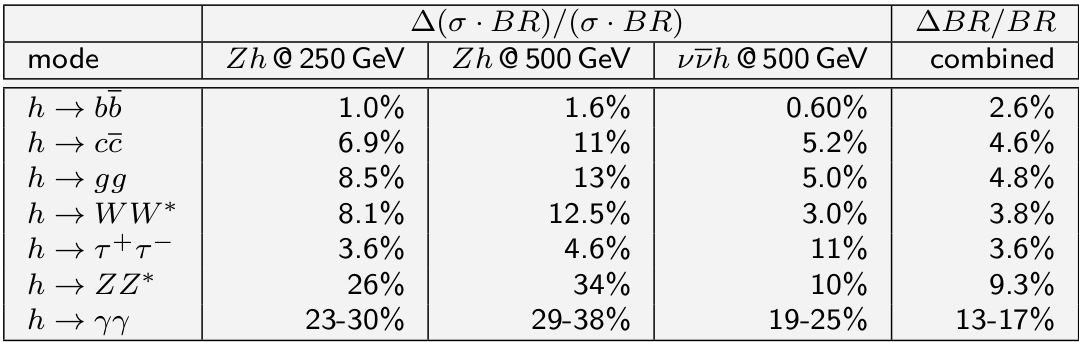
\includegraphics[scale=0.38]{./figures/BR_Higgs_500GeV.png}
      \caption{Pr\'ecisions sur les rapports de branchement mesur\'es \`a l'ILC en fonction des statistiques engrang\'ees \`a 250, 500, et 250+500 GeV.(source : TDR : Physics, page 39)}
     \label{fig:BR_500GeV}
     \end{center}
  \end{figure} 
   
   Toujours \`a 500 $GeV$, la d\'etermination des rapports de branchement du Higgs sera plus pr\'ecise en raison de l'augmentation de la statistique. La figure \ref{fig:BR_500GeV} r\'esume les pr\'ecisions atteignables en fonction de la luminosit\'e int\'egr\'ee \`a 250 et 500 $GeV$.   
   
%    De plus, pour tester si le Higgs est standard ou non, un test important est celui du potentiel de Higgs. Le potentiel du mod\`ele standard donne lieu \`a des auto-couplages triples et quadruples du Higgs. L'ILC mesurera le terme d'auto-couplage triple \cite{Baer:2013cma}.
   
   \medskip

  \begin{figure}[!htb]
    \begin{center} 
      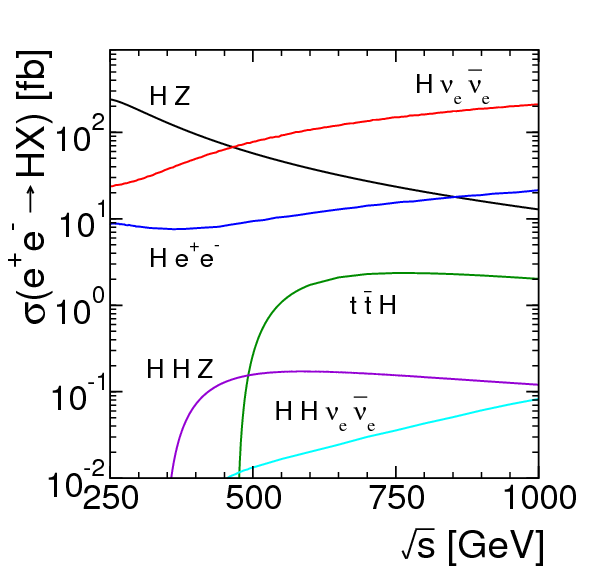
\includegraphics[scale=0.40]{./figures/cross_section_prod_Higgs_ILC.png}
      \caption{Section efficace de production du boson de Higgs. Les processus minoritaires sont cette fois-ci indiqu\'es.}
     \label{fig:crossSectionHiggs}
     \end{center}
  \end{figure} 
   
   Comme la figure \ref{fig:crossSectionHiggs} le montre, la section efficace de la r\'eaction $e^+ e^- \rightarrow t \overline{t} h$ augmente avec l'\'energie dans le centre de masse et atteint son maximum \`a environ 800 $GeV$. Cette section efficace d\'ecroît ensuite tr\`es l\'eg\`erement, mais reste proche de son maximum \`a 1 $TeV$. De plus, \`a 1 $TeV$ le bruit de fond $e^+ e^- \rightarrow t\overline{t}$ est devenu moins important. Une am\'elioration sur la pr\'ecision du coulage de Yukawa du quark top est alors possible. Une estimation r\'ecente r\'ealis\'ee grâce \`a une simulation compl\`ete, donne une pr\'ecision statistique de $4.0\%$ sur la valeur du couplage de Yukawa du top avec un Higgs standard de 125 $GeV$ et 1 $ab^{-1}$ de donn\'ees \`a 1 $TeV$ (voir TDR : physics, page 40).
   
   \medskip
   
   Toujours \`a 1 $TeV$ la fusion $WW$ est devenue le canal majoritaire de production de boson de Higgs, et en optimisant la polarisation des faisceaux \`a $(Pe^- , Pe^+ ) =  (-0.8, +0.2)$, on peut atteindre une section efficace de production de 400 $fb$ pour un Higgs de 125 $GeV$. Ainsi, avec 1 $ab^{-1}$ de donn\'ees, on obtient $4 \times 10^5$ \'ev\'enements contenant un Higgs. Cela permettra de mesurer le canal de d\'esint\'egration $h \rightarrow \mu^+ \mu^-$. Des simulations r\'ecentes montrent qu'il sera possible de mesurer la section efficace $\sigma BR(h \rightarrow \mu^+ \mu^-)$ avec une pr\'ecision d'environ $32\%$ pour un Higgs \`a 125 $GeV$, une polarisation $ P(-0.8, +0.2)$ et 1 $ab^{-1}$ \`a 1 $TeV$ (TDR, Physics : page 40).
   
   \medskip
   
   De plus, la section efficace du processus $e^+ e^- \rightarrow \nu \overline{\nu} h h$ devient beaucoup plus importante \`a 1 $TeV$ qu'\`a 500 $GeV$. Elle atteint environ 0.1 $fb$ \`a 1 $TeV$ (voir figure \ref{fig:crossSectionHiggs}). L'analyse de ce canal, coupl\'ee avec celle du canal $e^+ e^- \rightarrow Z h h$ permettra d'am\'eliorer la pr\'ecision sur la mesure de l'auto-couplage du Higgs. Une simulation compl\`ete r\'ecente donne une pr\'ecision $\Delta \lambda / \lambda \approx 0.21$. Ce r\'esultat est obtenu pour le canal $e^+ e^- \rightarrow \nu \overline{\nu} h h$ avec 2 $ab^{-1}$ \`a 1 $TeV$ et une polarisation $(P e^- , P e^+ ) = (-0.8, +0.2)$ (voir TDR : physics, page 41).
   
   \medskip

   \begin{figure}[!htb]
    \begin{center} 
      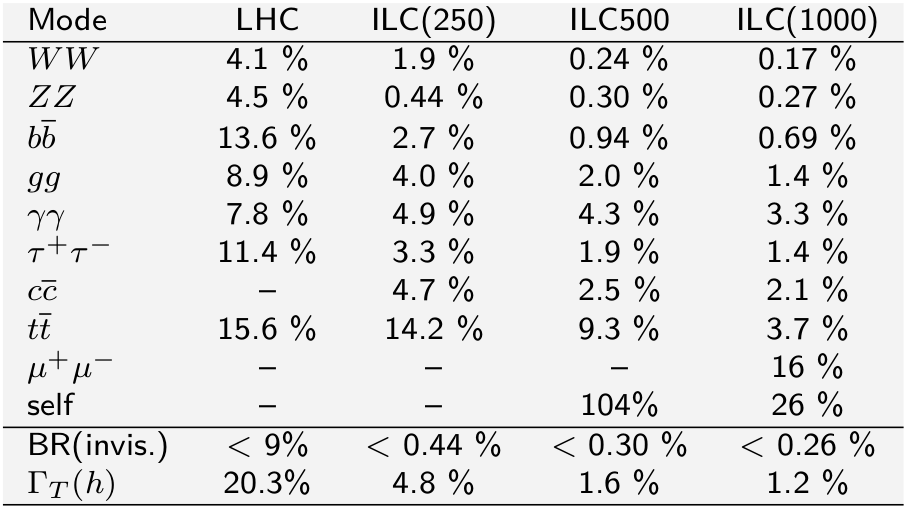
\includegraphics[scale=0.40]{./figures/Comparaison_couplage_1TeV.png}
      \caption{Pr\'ecisons sur les couplages du Higgs en fonction de l'exp\'erience, de l'\'energie dans le centre de masse et de la luminosit\'e int\'egr\'ee. \cite{Peskin:2012we}}
     \label{fig:Comp_BR_1000GeV}
     \end{center}
  \end{figure} 
   
   La figure \ref{fig:Comp_BR_1000GeV}, donne les diff\'erentes pr\'ecisions sur les couplages du Higgs. Sont mentionn\'ees les pr\'ecisions pour le LHC \`a 300 $fb^{-1}$ (avec 1 seul d\'etecteur), l'ILC \`a 250 GeV avec 250 $fb^{-1}$, l'ILC \`a 500 GeV avec 500 $fb^{-1}$ et l'ILC \`a 1000 GeV avec 1000 $fb^{-1}$ \cite{Peskin:2012we}. Cette figure r\'esume \`a elle toute seule l'int\'er\^et de l'ILC. Les pr\'ecisions obtenues \`a l'ILC permettront de tester si les param\`etres mesur\'es sont standards ou s'ils d\'evient du mod\`ele standard. La pr\'ecision de ces mesures constitue donc une sonde sur la physique au delà du mod\`ele standard.
   
   \subsubsection{Supersym\'etrie}
   
   Comme nous l'avons vu, la supersymétrie permet de r\'esoudre le probl\`eme de hi\'erarchie, elle postule un bon candidat de particule de mati\`ere noire et permet de faire se rejoindre les constantes de couplage des interactions fondamentales \`a l'\'echelle de grande unification.
   
   \medskip
   
   Actuellement (fin 2014), aucune preuve de particule supersym\'etrique n'a été identifiée au LHC, avec une \'energie de 8 $TeV$ dans le centre de masse. La recherche de telles particules au LHC continuera pour des \'energies de 13/14 TeV dans le centre de masse \`a partir de 2015. On notera que le LHC est particuli\`erement sensible aux super-partenaires color\'es.
   
   \medskip
   
   L'ILC sera un acc\'el\'erateur compl\'ementaire du LHC pour la recherche de supersymétrie. Il pourra permettre la mesure pr\'ecise d'\'eventuelles particules supersym\'etriques d\'ecouvertes au LHC. De plus, l'ILC permet de tester des espaces de param\`etres o\`u le LHC ne poss\`ede qu'une faible sensibilit\'e. Beaucoup de ces hypoth\'etiques nouvelles super-particules interagissent uniquement par l'interaction faible (neutralinos, jauginos). Leur faible niveau de production compar\'e aux particules interagissant par interaction forte, et le bruit de fond important des collisionneurs hadroniques, en font des particules difficilement observables au LHC. Ce bruit de fond et ce faible taux de production ne sont pas applicables au cas de l'ILC, et celui ci permettra de d\'ecouvrir et d'identifier ces particules si l'\'energie dans le centre de masse est assez haute pour les produire. Certaines particules supersym\'etriques ne lib\'erant qu'une tr\`es faible \'energie lors de leur d\'esint\'egration, le LHC, aura des difficult\'es \`a les d\'etecter. Ainsi, l'ILC gr\^ace \`a son faible bruit de fond pourrait d\'etecter des particules supersym\'etriques pass\'ees inaperçues au LHC. Pour finir, si de telles particules supersym\'etriques \'etaient d\'ecouvertes \`a l'ILC, ce dernier devrait fournir des mesures de pr\'ecisions sur les param\`etres les caract\'erisant, ce qui devrait fortement contraindre les mod\`eles th\'eoriques existants.

% \`a ses d\'etecteurs tr\`es pr\'ecis
   %   De nouvelles particules associ\'ees au champ de Higgs, \`a la mati\`ere noire mais aussi de nouvelles voies d'exploration en physique des particules permettront peut être de réaliser de nouvelles découvertes. La basse masse du boson de Higgs est myst\'erieuse. Ces corrections radiatives peuvent être corrig\'ees en ajoutant une nouvelle physique \`a l'\'echelle du $TeV$. Ceci est connu comme \'etant le \textit{probl\`eme de hi\'erarchie}. L'ILC recherchera les particules associ\'ees \`a cette nouvelle physique. Beaucoup de ces hypoth\'etiques nouvelles particules interagissent uniquement par l'interaction faible. Leur faible niveau de production compar\'e aux particules interagissant par interaction forte et le bruit de fond important des collisionneurs hadroniques en font des particules difficilement observables au LHC. Ce bruit de fond et ce faible taux de production ne sont pas applicable au cas de l'ILC, et celui ci permettra de d\'ecouvrir et d'identifier ces particules si elles poss\`edent une masse au moins aussi importante que l'énergie du faisceau.
%   
%   \medskip
%   
%   Parmi les mod\`eles de nouvelle physique \cite{Baer:2013cma} se trouve la supersym\'etrie. Ce mod\`ele résout le probl\`eme de la hi\'erarchie et est bas\'ee sur des sym\'etries d'espace-temps et entre fermions et bosons. La supersym\'etrie introduit des particules super-partenaires pour chaque particule du mod\`ele standard. Les corrections radiatives de ces super-partenaires introduisent de nouveaux termes pour la masse du (des) boson(s) de Higgs qui peuvent supprimer la divergence des corrections radiatives \`a sa masse \`a grande \'echelle. La recherche de ces nouvelles particules est au premier plan du programme du LHC. Actuellement, aucune preuve de particule supersym\'etriques n'a été identifié pour une \'energie de 8 $TeV$ dans le centre de masse. La recherche de telles particules au LHC continuera pour des \'energies de 13/14 TeV dans le centre de masse. Le LHC est particuli\`erement sensible aux super-partenaires color\'es (interagissant par interaction forte).
%   
%   \medskip
% 
%   La supersym\'etrie introduit de nouvelles particules de Higgs. Parmi celles-ci se trouvent 3 particules neutres ($h^0$ $H^0$ et $A^0$). Elles devraient \^etre difficiles \`a observer au LHC. L'existence de ces particules neutres est aussi motiv\'e par le rôle potentiel qu'elles peuvent jouer dans la compr\'ehension de la mati\`ere noire. Ces particules sont rarement produites et ne lib\`erent que tr\`es peu d'\'energie. Par rapport au LHC, ces particules seront facilement d\'etectable \`a l'ILC. De plus, l'ILC pourra mesurer leurs nombres quantiques et d\'eterminer leurs couplages \`a quelques pourcents pr\`es.
%   
%   \medskip
%   
%   L'ILC permettra des mesures de pr\'ecision des nouvelles particules d\'ecouvertes au LHC. Par exemple, l'ILC mesurera $\tan(\beta)$ pour le boson de Higgs ou $\cos(\theta_t)$ pour les partenaires supersym\'etriques du quark top, le tout de fa\c{c}on quasi- ind\'ependante des mod\`eles de physique. L'ILC devrait d\'elivrer des analyses plus fines et plus informative que le LHC en plus de potentielles nouvelles d\'ecouvertes. Les pr\'ecisions sur de telles nouvelles particules sont list\'ees en table \ref{tab:NewSummary}.
   
   
%    The precision measurements available at the ILC will provide a window to physics at much higher
% energy scales, possibly those associated with grand unification and string theory. The ILC will also
% provide a key connection between particle physics and cosmology, especially in identifying the nature
% of dark matter and shedding light on possible mechanisms for baryogenesis.
% Supersymmetry is challenged by the new results from the LHC, but this theory is still very
% attractive for the answers that it gives to the pressing theoretical problems of the Standard Model.
% The constraints from the LHC guide us to new regions of the large parameter space of supersymmetry.
% The ILC will explore these regions definitively and make precise measurements of new particles that
% may be found there. From this perspective, the construction of an ILC is more highly motivated now
% than ever before.


%   
%   \medskip
% 
%   La supersym\'etrie introduit de nouvelles particules de Higgs. Parmi celles-ci se trouvent 3 particules neutres ($h^0$ $H^0$ et $A^0$). Elles devraient \^etre difficiles \`a observer au LHC. L'existence de ces particules neutres est aussi motiv\'e par le rôle potentiel qu'elles peuvent jouer dans la compr\'ehension de la mati\`ere noire. Ces particules sont rarement produites et ne lib\`erent que tr\`es peu d'\'energie. Par rapport au LHC, ces particules seront facilement d\'etectable \`a l'ILC. De plus, l'ILC pourra mesurer leurs nombres quantiques et d\'eterminer leurs couplages \`a quelques pourcents pr\`es.
%   
%   \medskip
%   
%   L'ILC permettra des mesures de pr\'ecision des nouvelles particules d\'ecouvertes au LHC. Par exemple, l'ILC mesurera $\tan(\beta)$ pour le boson de Higgs ou $\cos(\theta_t)$ pour les partenaires supersym\'etriques du quark top, le tout de fa\c{c}on quasi- ind\'ependante des mod\`eles de physique. L'ILC devrait d\'elivrer des analyses plus fines et plus informative que le LHC en plus de potentielles nouvelles d\'ecouvertes. Les pr\'ecisions sur de telles nouvelles particules sont list\'ees en table \ref{tab:NewSummary}.
%   
%  \begin{table}[h]
%  \begin{center}
%  \caption{Exemples de mesures pr\'ecises des nouvelles particules r\'ealisables \`a l'ILC.}
%  \begin{tabular}{lccl}
%  Particule          &   Param\`etres & Pr\'ecision  $\Delta X/X$   
%   \\  \hline \hline
%  $ H^0$, $A^0$     &       $ m_H$, $m_A$  &   1.5\%   &  \\ 
%                             &   $\tan\beta$          &    20\%    &
%                             \\ 
%   $ \widetilde \chi^+       $            &
%   $  m(\widetilde\chi^+)   $   &    1\%     &  \\
%               &
%   $  m(\widetilde\chi^0)   $   &    1\%     &  \\
%   $ \widetilde t      $            &
%   $  m(\widetilde t)   $   &    1\%     &  \\
%   &   $   \cos\theta_t    $     &     0.4\%   \\ 
%  \end{tabular}
%  \label{tab:NewSummary}
%  \end{center}
%  \end{table}
   
   
%     \medskip
%    
%   La recherche de nouvelles particules sera aussi au programme. La recherche de particules supersym\'etriques singulet de couleur et l'exploration des \'etats associ\'es avec un secteur de Higgs \'etendu seront beaucoup moins difficile qu'au LHC. 
%   
%    La supersym\'etrie introduit de nouvelles particules de Higgs. Parmi celles-ci se trouvent 3 particules neutres ($h^0$ $H^0$ et $A^0$). Le boson trouv\'e au LHC pourrait \^etre l'un de ceux-ci. L'existence de ces particules neutres est aussi motiv\'e par le rôle potentiel qu'elles peuvent jouer dans la compr\'ehension de la mati\`ere noire. Ces particules sont rarement produites et ne lib\`erent que tr\`es peu d'\'energie. Par rapport au LHC, ces particules seront facilement d\'etectable \`a l'ILC. De plus, l'ILC pourra mesurer leurs nombres quantiques et d\'eterminer leurs couplages \`a quelques pourcents pr\`es.
%    \medskip
%    
%    Une seconde \'etape sera la mesure de grande précision des paramètres et des couplages des autres particules du mod\`ele standard. Ces deux \'etapes, qui demandent des mesures de pr\'ecision, ne sont r\'ealisables qu'avec un collisionneur d'\'electrons et de positons (ou de leptons) et non de hadrons. De plus, des recherches de nouvelles particules seront bien entendu effectu\'ees au cours de ce programme. Le tableau \ref{tab:ILCprogramX} illustre diff\'erents exemples de points de fonctionnements de l'ILC en fonction de l'\'energie dans le centre de masse et des objectifs de physique vis\'es. \cite{Behnke:2013xla}
% 
% 
%  
% 
% 
% %   \medskip
% %   
% %   Le programme de physique de l'ILC devrait d\'ebuter \`a une énergie d'environ 250 $GeV$ dans le centre de masse, puis il devrait \^etre mis \`a jour par \'etape pour atteindre une \'energie d'environ 500 $GeV$ dans le centre de masse ce qui constitue l'\'energie nominale du projet. Une extension \`a 1 $TeV$ est envisag\'ee. Cependant celle-ci n'aura lieu qu'\`a la toute fin du programme de physique.
%   
%   \medskip
%   
% 
%   
%   \medskip
%   
%    
%   
%   \begin{figure}[!htb]
%     \begin{center} 
%       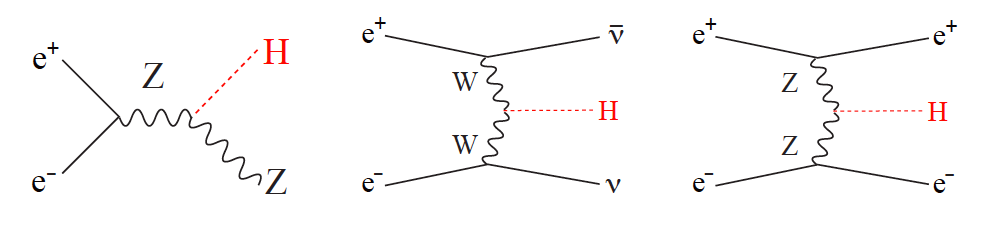
\includegraphics[scale=0.40]{./figures/feynman_Higgs.png}
%       \caption{Diagrammes de Feynman pour les 3 processus majeurs de production de Higgs \`a l'ILC : $e^+ e^- \rightarrow Z h$ (\`a gauche), $e^+ e^- \rightarrow \nu \overline{\nu} h$ (au centre), et $e^+ e^- \rightarrow e^+ e^- h$ (\`a droite). }
%       \label{fig:feynmanHiggs2}
%     \end{center}
%   \end{figure} 
%   
%   \begin{figure}[!htb]
%     \begin{center} 
%       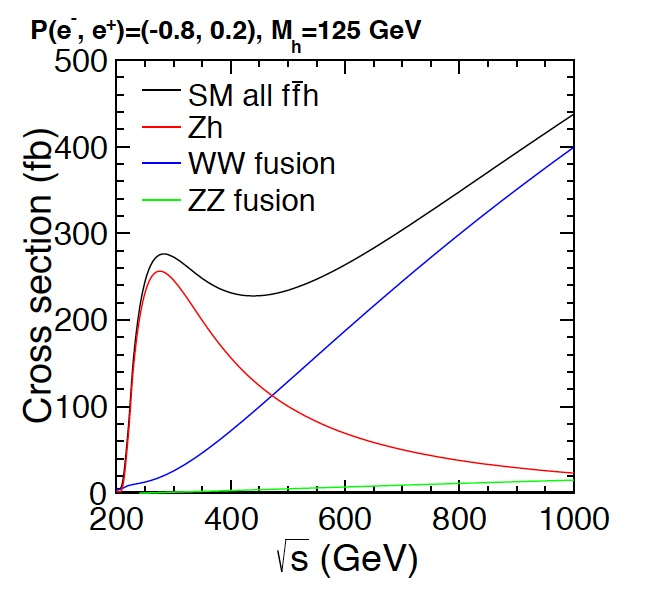
\includegraphics[scale=0.40]{./figures/energy_Higgs.jpg}
%       \caption{Section efficace de production pour le Higgstrahlung ($e^+ e^- \rightarrow Z h$), la fusion WW ($e^+ e^- \rightarrow \nu \overline{\nu} h$) et la fusion ZZ ($e^+ e^- \rightarrow e^+ e^- h$) en fonction de l'\'energie dans le centre de masse, pour une masse du Higgs de 125 $GeV$, et pour une polarisation de faisceau ($P_{e^-}$, $P_{e^+}$) = ($-0.8$, $+0.2$). }
%      \label{fig:energyHiggs}
%      \end{center}
%   \end{figure}   
%   
%   Entre environ 200 et 450 $GeV$ le processus dominant est le Higgstrahlung. Celui-ci croit entre environ 200 et 275 $GeV$ puis diminue lentement par la suite. Comme le processus de fusion $WW$ augmente de façon quasi-r\'eguli\`ere, il devient dominant \`a partir d'environ 450 $GeV$. La fusion ZZ est quant \`a elle tr\`es minoritaire. La facult\'e de r\'ealiser des mesures de pr\'ecision de ces processus \`a l'ILC résulte d'une bonne connaissance des \'etats initiaux et de niveaux de signal-sur-bruit \'elev\'e. 
%   
%   \medskip
%   
%   Le programme de l'ILC devrait donc commencer par l'exploitation du pic du higgsstrahlung vers 250 $GeV$. Pour cela, la masse de recul du Higgs $M_H$ sera reconstruite. Cette masse est ind\'ependante de toutes hypoth\`eses sur les produits de d\'esint\'egration du Higgs. La masse de recul est calcul\'ee selon la relation suivante :
%   
%   \begin{equation}
%    M_H^2 = s + M_Z^2 - 2 \sqrt{s}(E_1 + E_2)
%   \end{equation}
% 
%   o\`u $M_H$ est la masse de recul du boson de Higgs, $M_Z$ la masse du boson $Z$ et $E1$ et $E2$ sont les \'energies des produits de d\'esint\'egration du $Z$.
%   La figure \ref{fig:simuILC}(a) montre une simulation d'un \'ev\`enement Higgsstrahlung, ou le Z se d\'esint\`egre en une paire de muons $\mu^+ \mu^-$ et o\`u le Higgs donne une paire de quark $b \overline{b}$. La figure \ref{fig:simuILC}(b) repr\'esente quant \`a elle la simulation bas\'ee sur 250 $fb^{-1}$ de donn\'ees, de la masse de recul du Higgs dans le cas ou le Z se d\'esint\`egre en une paire de muons $\mu^+ \mu^-$.
% 
%   \medskip
%   
%   Ainsi, les taux de d\'esint\'egration du boson de Higgs pourront \^etre mesur\'e avec pr\'ecision. Ces mesures incluent des d\'esint\'egrations invisibles ou des \'etats finals inhabituels. Compar\'e au LHC o\`u de tels \'ev\`enements sont tr\`es difficilement s\'eparables du bruit de fond du mod\`ele standard, l'ILC permettra ces mesures avec une grande pr\'ecision. Ces mesures de grande pr\'ecisions des taux de d\'esint\'egration du boson de Higgs selon diff\'erentes voies (quarks, leptons et bosons) permettront de savoir si seul le champs de Higgs conf\`erent leur masse aux particules \'el\'ementaires ou si d'autres particules partagent le rôle de g\'en\'erateur de la masse. Il existe en effets plusieurs sc\'enarios de  nouvelle physique qui g\'en\`erent des d\'eviations inf\'erieure \`a 10$\%$ par rapport au mod\`ele standard \cite{Gupta:2013}.
%   
%   
%   \begin{figure}[!htb]
%     \begin{center} 
%       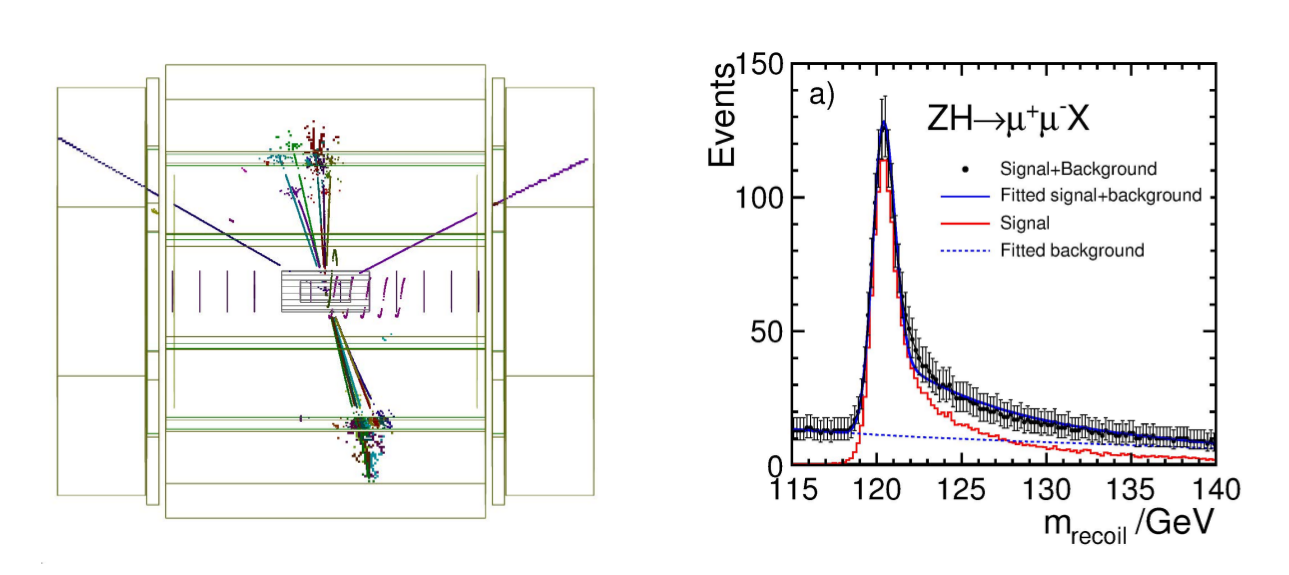
\includegraphics[scale=0.30]{./figures/figure_ilc_barish_brau.png}
%       \caption{(a) Simulation d'un \'ev\`enement $e^+ e^- \rightarrow Z h$, avec $Z \rightarrow \mu^+ \mu^-$ et $h \rightarrow b\overline{b}$, comme attendu au d\'etecteur ILD de l'ILC. (b) R\'esultats d'une simulation de 250 $fb^{-1}$ du Higgsstrahlung $e^+ e^- \rightarrow Z h$ avec $Z \rightarrow \mu^+ \mu^-$ comme attendu dans le d\'etecteur ILD de l'ILC. }
%     \label{fig:simuILC}
%     \end{center}
%   \end{figure}
%   
%   \medskip
%   
%   Le programme de mesure \`a 250 $GeV$ inclura la mesure de la masse mais aussi du spin du boson de Higgs. Ainsi, la masse de recul comme illustr\'ee en figure \ref{fig:simuILC}(b) permet d'obtenir une pr\'ecision statistique de l'ordre de 40 $MeV$ sur la masse de recul du Higgs pour le canal $Z \rightarrow \mu^+ \mu^-$ avec une \'energie de 250 $GeV$ dans le centre de masse et 250 $fb^{-1}$ de donn\'ees simul\'ees. Une pr\'ecision de l'ordre de 80 $MeV$ est obtenue dans les m\^eme condition de simulation pour le canal $Z \rightarrow e^+ e^-$. La combinaison des deux r\'esultats donne une pr\'ecision sur la mesure d'environ 35 $MeV$.
%   
%   \medskip
%   
%   L'ILC procurera aussi un test complémentaire avec le LHC pour la mesure du spin du boson de Higgs. Le comportement au seuil de production pour la section efficace $e^+ e^- \rightarrow Zh$ ne varie pas de la m\^eme mani\`ere selon les valeurs du spin et de CP pour le boson de Higgs. La possibilit\'e d'un spin 1 a \'et\'e exclue par l'observation du canal $h\rightarrow \gamma \gamma$ au LHC. Cette voie de d\'esint\'egration impose une valeur positive pour la conjugaison de charge. Pour un boson de Higgs de spin 0, le comportement au seuil de la section efficace $e^+ e^- \rightarrow Zh$ \`a l'ILC varie comme $\beta$ pour une valeur de CP paire et comme $\beta^3$ pour une valeur de CP impaire. Pour un boson de Higgs de spin 2, la section efficace au seuil augmente comme $\beta^3$. Pour des spin plus \'elev\'es, la section efficace au seuil augmentera selon des puissances de $\beta$ plus grande que 3. Une mesure de la section efficace \`a trois points juste au dessus du seuil devrait permettre de trancher entre toutes ces possibilit\'es.
%   
%   \medskip
%   
%   \`A des \'energies bien au dessus du seuil (350 $GeV$), le processus $e^+ e^- \rightarrow Zh$ devrait \^etre domin\'e par la production longitudinale de boson Z. Cela sera utilis\'e pour confirmer la nature scalaire du boson de Higgs. L'ILC sera aussi capable de traiter des cas plus compliqu\'es comme, par exemple, celui d'un Higgs qui n'est pas un \'etat propre de CP mais un m\'elange d'\'etats propres de CP pairs et impairs. L'environnement unique et le param\'etrage des faisceaux font de l'ILC un outil puissant pour tester ces possibilit\'es.\cite{Baer:2013cma}
%   
%   \medskip
%   
%   La section efficace du processus $e^+ e^- \rightarrow Zh$ avec $h \rightarrow ZZ$constitue une mesure directe du couplage $g_{hZZ}$. La largeur du processus de d\'esint\'egration $h \rightarrow ZZ$, $\Gamma(h \rightarrow ZZ)$ est proportionnelle \`a la section efficace $e^+ e^- \rightarrow Zh$. Étant donn\'e le rapport de branchement $BR(h \rightarrow ZZ)$ obtenu gr\^ace \`a la m\'ethode de la masse de recul, la largeur du boson de Higgs est donn\'ee par : 
%   
%   \begin{equation}
%    \Gamma_{tot} = \dfrac{\Gamma(h \rightarrow ZZ)}{BR(h \rightarrow ZZ)}
%   \end{equation}
% 
%   Dans le mod\`ele standard, cette largeur vaut environ 4 $MeV$. La pr\'ecision sur cette mesure sera d'environ 2$\%$ \`a 250 $GeV$ et 250 $fb^{-1}$ de donn\'ees plus 500 $fb^{-1}$ de donn\'ee \`a 500 $GeV$.
%   
%   \medskip
% 
%   \`A la suite du programme de la mesure des param\`etres du boson de Higgs \`a 250 GeV, le programme de physique continuera \`a des \'energies plus hautes. Un pallier \`a 350 GeV devrait \^etre effectu\'e. A ce niveau d'\'energie, la section efficace de production de paires de quark top apparaît. L'augmentation de cette section efficace est pr\'ecis\'ement pr\'edite grâce aux calculs de QCD perturbative et gr\^ace aux mesures d\'ej\`a effectu\'ees. Ceci m\`enera \`a la d\'etermination de la masse du quark top avec une pr\'ecision de l'ordre de 100 MeV. Une telle pr\'ecision n'est pas atteignable au LHC. Cette mesure est cruciale pour les pr\'edictions de physique fondamentale comme celles des th\'eories de grande unification. De plus la mesure d\'etaill\'ee des \'ev\`enements mettant en jeu des paires de quark top proche du seuil de production et au-dessus de celui-ci va permettre la mesure pr\'ecise de certains param\`etres de la th\'eorie de la brisure de sym\'etrie \'electrofaible. Avec son faisceau polarisable, l'ILC devrait \^etre sensible \`a de la nouvelle physique et en particulier \`a un boson de Higgs composite.
%   
%   \medskip
%   
%   Dans la région d'\'energie 350-400 $GeV$ dans le centre de masse, la r\'eaction $e^+ e^- \rightarrow WW$ permettra de sonder le mod\`ele standard \`a haute \'energie. Au fur et \`a mesure que l'\'energie monte, le processus de fusion $WW$ ($e^+ e^- \rightarrow \nu \overline{\nu} h$) cro\^it et une mesure du couplage $hWW$ est alors possible. Il s'agit d'une des valeurs cruciales dans l'\'etude pr\'ecise du boson de Higgs. 
%   
%   \medskip
%   
%   A son \'energie nominale de 500 $GeV$ la section efficace du processus de fusion $WW$ est encore plus \'elev\'ee comme l'atteste la figure \ref{fig:energyHiggs}. Ceci permettra une mesure encore plus pr\'ecise des couplages au Higgs. A 500 $GeV$ l'ILC sera sensible \`a l'auto-couplage du Higgs. A cette \'energie, des \'etudes pr\'ecise des r\'eactions $e^+ e^- \rightarrow f\overline{f}$ seront effectu\'ees avec une grande sensibilit\'e. Ainsi l'exploration des r\'esonances \`a grande masse des bosons vecteurs, des nouvelles interactions fermioniques, et des quarks et leptons composites sera effectu\'ee. La recherche de nouvelles particules sera aussi au programme. La recherche de particules supersym\'etriques singulet de couleur et l'exploration des \'etats associ\'es avec un secteur de Higgs \'etendu seront beaucoup moins difficile qu'au LHC.
%   
%   \medskip
%   
%   L'\'etude des productions de paires de quarks, de leptons, et de bosons W et Z \`a l'ILC devrait permettre d'obtenir de nouvelles connaissances sur de possibles nouvelles interactions \`a des niveaux de masse plus \'elev\'e.
%   
%   \medskip
%   
%   L'\'etude d\'etaill\'ee des propri\'et\'es du boson W et du quark top seront ajout\'es \`a notre connaissance actuelle des mesures de pr\'ecision sur le boson Z, obtenues gr\^ace aux collisionneurs $e^+ e^-$. Parmi ces mesures, une mesure de la masse du quark top avec une précision de 100 $MeV$ fourni gr\^ace \`a une analyse en seuil, devrait \^etre obtenue \`a l'ILC. Cette mesure constitue un param\`etre important \`a connaître pour effectuer des calculs th\'eoriques pr\'ecis. Les pr\'ecisions sur les mesures du quark top et du boson W sont fournis en table \ref{tab:TopSummary}
%   
%   \begin{table}[h]    %[p] 
%   \begin{center}
%   \caption{Pr\'ecision sur les param\`etres cl\'ees du quark top et du boson W du mod\`ele standard \`a l'ILC.}
%   \begin{tabular}{lccl}
%   Particule          &   Param\`etre & Pr\'ecision  $\Delta X/X$   
%   \\  \hline \hline
%   Top           &    $  m_t   $  &      0.02\%   &   $\Delta m_t =
%   30$~MeV,   balayage en seuil \\ 
% 		      &     $\Gamma_t  $&   2.\%     &    \\ 
% 			&    $\tilde F^\gamma_{1V} $      &    0.2\%     &      500
% 			GeV\\ 
% 			&    $\tilde F^Z_{1V} $      &    0.3\%     &     \\
% 			&    $\tilde F^Z_{1A} $      &    0.5\%     &     \\
% 			&    $\tilde F^\gamma_{2V} $      &    0.3\%     &     \\
% 			&    $\tilde F^Z_{2V} $     &    0.6\%     &
% 			\\ \hline
%   $W$          &    $  m_W   $  &      0.004\%   &   $\Delta m_W =
%   3$~MeV,   balayage en seuil \\ 
% 			&    $ g_1  $&   0.16\%     &   500~GeV \\ 
% 			&    $\kappa_\gamma $      &    0.03\%     &     \\ 
% 			&    $\kappa_Z  $      &    0.03\%     &     \\  
% 			&    $\lambda_\gamma $      &    0.06\%     &     \\ 
% 			&    $\lambda_Z  $      &    0.07\%     &     \\
%   \end{tabular}
%   \label{tab:TopSummary}
%   \end{center}
%   \end{table}
% 
%   Lorsque l'\'energie augmente et atteint 1 $TeV$ dans le centre de masse, une mesure pr\'ecise des couplages de Yukawa du boson de Higgs avec le quark top est possible. La mesure de l'autocouplage du Higgs \`a cette \'energie atteindra une pr\'ecision de 20 $\%$. Le programme de recherche de nouvelles particules exotiques continuera et la recherche de Higgs interagissant fortement ou de Higgs composite sera possible. Le quark top offre un indicateur possible de la pr\'esence d'une structure composite pour le Higgs qui pourrait \^etre observ\'ee dans la mesure des couplages forts du quark top au champ de Higgs.
%   
%   \medskip
%   
%   La table \ref{tab:HiggsSummary} r\'esume les pr\'ecisions qui pourront \^etre obtenues \`a l'ILC pour la physique du Higgs.\cite{Behnke:2013xla} Ce tableau est bas\'e sur les param\`etres de l'ILC donn\'es dans le TDR (\textit{Technical Design Report}).Ces pr\'esisions sont ind\'ependantes du mod\`ele choisi, \`a la diff\'erence des analyses d\'ependantes des mod\`eles fr\'equemment employ\'ees pour tester les diff\'erents couplages du mod\`ele standard. Par exemple, le LHC HXSWG (\textit{Higgs Cross Section Working Group}) propose pour les couplages du Higgs une série d'indicateurs de r\'ef\'erence \cite{Dittmaier:2011ti}, bas\'es sur certains mod\`eles comme le mod\`ele standard ou la supersym\'etrie. Lorsque de telles hypoth\`eses sont faites pour les mesures \`a l'ILC, des pr\'ecisions encore meilleures peuvent \^etre obtenues.
%   
%   \begin{table}[h]    %[p] 
%   \begin{center}
%   \caption{Estimation des mesures des propri\'et\'es du boson de Higgs du mod\`ele standard ($m_h = 125$ GeV). Ces analyses ne nécessitent pas d'hypoth\`eses significatives sur les mod\`eles de physique. Les pr\'ecisions sur les mesures \`a l'ILC sont obtenues avec des lots d'\'ev\`enement de 250 $fb^{-1}$ \`a 250 $GeV$, 500 $fb^-{1}$ \`a 500 GeV et 1000 $fb^-{1}$ \`a 1 $TeV$. La polarisation du faisceau $e^-/e^+$ est de 80$\%$/30$\%$ \`a 250 et 500 GeV et de 80$\%$/20$\%$ \`a 1 $TeV$.}
%   \begin{tabular}{lccl}
%   Particule          &   Param\`etres & Pr\'ecision  $\Delta X/X$   
%   \\  \hline \hline
%   Higgs            &   $  m_h $   &      0.03\%   &   $\Delta m_h =
%   35$~MeV,   250 GeV \\ 
% 		  &    $  \Gamma_h  $ &   2.\%     &     250 GeV and 500
% 		      GeV \\                     
% 		      &   $  g(hWW)  $  &  0.3\%    &        \\ 
% 		      &    $ g(hZZ)  $    &  0.35\%    &        \\ 
% 		      &    $ g(hb\bar b)  $ &  1.1\%    &        \\ 
% 		      &    $ g(hc \bar c)  $ &  2.1\%    &        \\ 
% 		      &    $ g(hgg)  $ &  2.3\%    &        \\ 
% 		      &    $ g(h\tau^+\tau^-)  $ &  2.0\%    &        \\ 
% 		      &   $  BR(h\to \mbox{ invis.})  $ &   0.05\%  &
% 		      \\ 
% 			&    $ g(ht\bar t)  $  &  4.5\%    &    1000 GeV    \\ 
% 			&    $ g(hhh)  $  &  20.\%    &     \\ 
% 		      &   $  g(h\mu^+\mu^-)  $ &  16.\%    &        \\  
% 
%   \end{tabular}
%   \label{tab:HiggsSummary}
%   \end{center}
%   \end{table}
% 
%   De nouvelles particules associ\'ees au champ de Higgs, \`a la mati\`ere noire mais aussi de nouvelles voies d'exploration en physique des particules permettront peut être de réaliser de nouvelles découvertes. La basse masse du boson de Higgs est myst\'erieuse. Ces corrections radiatives peuvent être corrig\'ees en ajoutant une nouvelle physique \`a l'\'echelle du $TeV$. Ceci est connu comme \'etant le \textit{probl\`eme de hi\'erarchie}. L'ILC recherchera les particules associ\'ees \`a cette nouvelle physique. Beaucoup de ces hypoth\'etiques nouvelles particules interagissent uniquement par l'interaction faible. Leur faible niveau de production compar\'e aux particules interagissant par interaction forte et le bruit de fond important des collisionneurs hadroniques en font des particules difficilement observables au LHC. Ce bruit de fond et ce faible taux de production ne sont pas applicable au cas de l'ILC, et celui ci permettra de d\'ecouvrir et d'identifier ces particules si elles poss\`edent une masse au moins aussi importante que l'énergie du faisceau.
%   
%   \medskip
%   
%   Parmi les mod\`eles de nouvelle physique \cite{Baer:2013cma} se trouve la supersym\'etrie. Ce mod\`ele résout le probl\`eme de la hi\'erarchie et est bas\'ee sur des sym\'etries d'espace-temps et entre fermions et bosons. La supersym\'etrie introduit des particules super-partenaires pour chaque particule du mod\`ele standard. Les corrections radiatives de ces super-partenaires introduisent de nouveaux termes pour la masse du (des) boson(s) de Higgs qui peuvent supprimer la divergence des corrections radiatives \`a sa masse \`a grande \'echelle. La recherche de ces nouvelles particules est au premier plan du programme du LHC. Actuellement, aucune preuve de particule supersym\'etriques n'a été identifié pour une \'energie de 8 $TeV$ dans le centre de masse. La recherche de telles particules au LHC continuera pour des \'energies de 13/14 TeV dans le centre de masse. Le LHC est particuli\`erement sensible aux super-partenaires color\'es (interagissant par interaction forte).
%   
%   \medskip
% 
%   La supersym\'etrie introduit de nouvelles particules de Higgs. Parmi celles-ci se trouvent 3 particules neutres ($h^0$ $H^0$ et $A^0$). Elles devraient \^etre difficiles \`a observer au LHC. L'existence de ces particules neutres est aussi motiv\'e par le rôle potentiel qu'elles peuvent jouer dans la compr\'ehension de la mati\`ere noire. Ces particules sont rarement produites et ne lib\`erent que tr\`es peu d'\'energie. Par rapport au LHC, ces particules seront facilement d\'etectable \`a l'ILC. De plus, l'ILC pourra mesurer leurs nombres quantiques et d\'eterminer leurs couplages \`a quelques pourcents pr\`es.
%   
%   \medskip
%   
%   L'ILC permettra des mesures de pr\'ecision des nouvelles particules d\'ecouvertes au LHC. Par exemple, l'ILC mesurera $\tan(\beta)$ pour le boson de Higgs ou $\cos(\theta_t)$ pour les partenaires supersym\'etriques du quark top, le tout de fa\c{c}on quasi- ind\'ependante des mod\`eles de physique. L'ILC devrait d\'elivrer des analyses plus fines et plus informative que le LHC en plus de potentielles nouvelles d\'ecouvertes. Les pr\'ecisions sur de telles nouvelles particules sont list\'ees en table \ref{tab:NewSummary}.
%   
%  \begin{table}[h]
%  \begin{center}
%  \caption{Exemples de mesures pr\'ecises des nouvelles particules r\'ealisables \`a l'ILC.}
%  \begin{tabular}{lccl}
%  Particule          &   Param\`etres & Pr\'ecision  $\Delta X/X$   
%   \\  \hline \hline
%  $ H^0$, $A^0$     &       $ m_H$, $m_A$  &   1.5\%   &  \\ 
%                             &   $\tan\beta$          &    20\%    &
%                             \\ 
%   $ \widetilde \chi^+       $            &
%   $  m(\widetilde\chi^+)   $   &    1\%     &  \\
%               &
%   $  m(\widetilde\chi^0)   $   &    1\%     &  \\
%   $ \widetilde t      $            &
%   $  m(\widetilde t)   $   &    1\%     &  \\
%   &   $   \cos\theta_t    $     &     0.4\%   \\ 
%  \end{tabular}
%  \label{tab:NewSummary}
%  \end{center}
%  \end{table}
%  
%   \medskip
  
  \subsubsection{Conclusion}
  
  Comme illustr\'e dans cette section, l'ILC explorera les plus importantes questions en physique des particules en mesurant avec une pr\'ecision encore in\'egal\'ee les param\`etres des particules \'el\'ementaires. Ainsi, l'ILC devrait offrir des mesures du boson de Higgs, des bosons W et Z, du quark top et des nouvelles particules au delà du mod\`ele standard qui seront peut-\^etre d\'ecouvertes au LHC ou \`a l'ILC.
  
  \medskip
  
  Pour r\'ealiser ce programme de physique ambitieux, l'ILC requiert de nouvelles avanc\'ees en termes de performances de d\'etection par rapport aux détecteurs de particules anciens et actuels. En vertu du niveau de pr\'ecision que devra atteindre l'ILC et du faible bruit de fond compar\'e au LHC, de meilleures technologies de d\'etection, encore plus pr\'ecises, doivent \^etre envisag\'ees. Examinons \`a pr\'esent les performances que devront fournir les d\'etecteurs de l'ILC.
  
%   \subsection{Bruit de fond}
%   
%   Beanstrahlung \\
%   Taux d'occupation \\
  
%   \subsection{D\'etecteurs}
%   
%   Historiquement 2 d\'etecteurs. Mais maintenant : Un ou peut-\^etre deux ? ... \\
%   ILD et SID : 2 voies diff\'erentes \\
%   
%   \subsubsection{ILD}
%   
%   D\'etecteur de Vertex \\
%   Trajectom\`etre \\
%   Colorim\`etres \\
%   Champs magn\'etique et culasse (+ muons) \\
  
%\section[Physique \`a l'ILC]{Physique \`a l'ILC\protect\footnote{Cette section est tir\'ee en grande partie de l'article de \textit{Barish} et \textit{Brau} : \textit{The International Linear Collidor} \cite{BARISH:2013}.}}
% 
%   L'ILC ou \textit{International Linear Collider} devrait jouer un r\^ole central pour la physique des particules de demain. Il s'agit d'un collisionneur lin\'eaire d'\'electrons et de positons dot\'e d'une \'energie dans le centre de masse de 200-500 $GeV$ (extensible \`a 1 $TeV$), d'une haute luminosit\'e, et d'une technologie acc\'el\'eratrice \`a radio-fr\'equences \`a base de supraconducteurs (SCRF). Il pourra permettre de nombreuses \'etudes de ph\'enom\`enes physiques encore inexplor\'es, comme la nouvelle physique, une \'etude pr\'ecise du quark top et bien sur l'\'etude fine du boson de Higgs, r\'ecemment d\'ecouvert au \textit{Large Hadron Collider} \cite{Aad:2012tfa, Chatrchyan:2012ufa}. Dans cette partie nous d\'ecrirons les objectifs de physique de l'ILC, nous verrons le fonctionnement de cet acc\'el\'erateur, puis nous expliciterons l'importance de ces ses diff\'erents d\'etecteurs.
% 
% \subsection{Objectifs de physique}
%   
  \subsection{D\'etecteurs}

  %Deux d\'etecteurs interchangeables sont envisag\'es pour l'$ILC$, le $SiD$ pour $Silicon$ $Detector$ et l'$ILD$ pour $International$ $Linear$ $Detector$. Nous nous intéresserons plus particuli\`erement \`a l'$ILD$.
  
%   Le programme de physique de l'ILC requiert de nouvelles avanc\'ees en termes de performances de d\'etection par rapport aux détecteurs de particules anciens et actuels. En vertu du niveau de pr\'ecision que devra atteindre l'ILC et du faible bruit de fond compar\'e au LHC, de meilleures technologies de d\'etections, encore plus pr\'ecises, doivent \^etre envisag\'ees.
  
  Une fois le programme de physique pass\'e en revue, la question de la d\'etection des ph\'enom\`enes physiques \`a \'etudier se pose. Étant donn\'e les faibles sections efficaces de production, la luminosit\'e du collisionneur et le bruit de fond machine, quel type de d\'etecteur doit-on construire pour s'assurer de mesurer les \'ev\'enements physiques recherch\'es ? C'est ce que nous allons expliciter dans cette partie. Premi\`erement nous listerons les diff\'erents pr\'e-requis pour les d\'etecteurs de l'ILC dict\'es par la physique. Puis, nous traiterons le cas du nombre de d\'etecteurs au niveau du point d'interaction. Ensuite, nous analyserons la structure du faisceau et le bruit de fond au niveau de la r\'egion d'interaction. Nous d\'ecrirons alors les diff\'erentes options de d\'etecteurs envisag\'ees pour la calorim\`etrie, la trajectom\'etrie et le d\'etecteur de vertex. Nous pr\'esenterons alors l'ILD, l'un des d\'etecteurs envisag\'e \`a l'ILC, et ses performances. Le d\'etecteur de vertex \'etant le d\'etecteur \'etudi\'e dans cette th\`ese, nous nous pencherons plus en d\'etail sur celui-ci.
  
%   en attachant un int\'erêt tout particulier au d\'etecteur de vertex. Ce dernier faisant partie int\'egrante de cette th\`ese.
  
  \subsubsection{Objectifs de physique et d\'etecteurs}
  
  Parmi les principales exigences sur la conception des d\'etecteurs, du cot\'e de la calorim\`etrie, se trouve la reconstruction avec une grande pr\'ecision de l'\'energie des \textit{jets} \footnote{Un jet est un ensemble de particules issus de l'hadronisation des quarks et gluons} et de la masse des \textit{di-jets}. Pour cela la technique du \textit{particle flow algorithm} (PFA) a \'et\'e choisie. Afin de s\'eparer les di-jets provoqu\'es soit par les bosons W soit par les bosons Z, la pr\'ecision sur la reconstruction de l'\'energie des jets issus de l'hadronisation de ces bosons, doit atteindre 3 \`a 4 $\%$ pour des jets de 100 $GeV$. 
  
  \medskip
  
  Pour la trajectom\'etrie (\textit{tracking}), la résolution sur l'impulsion des traces charg\'ees est d\'efinie par la pr\'ecision sur la reconstruction de la masse de recul du Higgs calcul\'ee dans le cas d'une d\'esint\'egration du boson Z en une paire lepton-antilepton. Ainsi, la masse du boson de Higgs, reconstruite selon la mesure sur la paire lepton-antilepton, devra offrir un rapport $\Delta p / p^2 < 5\times 10^{-5} (GeV/c)^{-1}$. 
  
  \medskip
  
  Enfin, pour le detecteur de vertex, l'identification de la saveur et de la charge des quarks devra \^etre effectu\'ee gr\^ace \`a une nouvelle g\'en\'eration de d\'etecteur de vertex.
  
  \medskip
  
  De plus, les calorim\`etres, hautement granulaires, devront participer \`a l'identification des particules et la d\'etection des muons sera suppl\'e\'ee par une culasse instrumentalis\'ee.
  
  \medskip
  
  Ces caract\'eristiques d\'epassent de loin les performances obtenues par les détecteurs des collisionneurs actuels, y compris ceux du LHC. Les conditions sp\'ecifiques \`a l'ILC (structure en temps du faisceau et bas niveau de radiation) rendent ces avanc\'ees possibles et de nombreux programmes de recherche et d\'eveloppement des d\'etecteurs ont vu le jour. De ces pr\'e-requis, deux concepts de d\'etecteurs pour l'ILC ont \'emerg\'e : le SiD \textit{Silicon Detector} et l'ILD \textit{International Large Detector}.
  
  \subsubsection{Un point d'interaction, deux d\'etecteurs ?}
  
%   Dans les collisionneurs de particules r\'ecents et actuels tel que le Tevatron, le LEP, HERA ou le LHC ; au moins deux d\'etecteurs sont mis en concurrence. Chaque d\'etecteur apporte une approche compl\'ementaire, une confirmation des r\'esultats d'un autre, une possibilit\'e de combinaison des donn\'ees, plus de fiabilit\'e et une assurance vis \`a vis d'une panne \'eventuelle d'un autre d\'etecteur. L'histoire montre que plusieurs d\'etecteurs valent mieux qu'un. Ainsi, lorsque l'exp\'erience UA1 d\'eclara avoir observ\'e des preuves de l'existence du quark top d'une masse d'environ 40 $GeV/c^2$, l'exp\'erience UA2 ne l'observa pas. Et c'est finalement en 1995 que le quark top fut d\'ecouvert au Tevatron par les exp\'eriences CDF et D0. 

  L'ILC a \'et\'e con\c{c}u pour accueillir deux d\'etecteurs compl\'ementaires, le \textit{SiD} et l'\textit{ILD}. Le \textit{SiD} et l'\textit{ILD} sont con\c{c}us pour \^etre g\'en\'eralistes et sont optimis\'es pour la large gamme de physiques possible \`a l'ILC. Le \textit{SiD} est un d\'etecteur compact bas\'e sur un syst\`eme de trajectom\`etrie en silicium et un champ magn\'etique de 5 Teslas, le tout r\'ealis\'e avec un co\^ut restreint. Les technologies bas\'ees sur le silicium permettent d'avoir une r\'esolution temporelle de l'ordre d'un croisement de paquets, ce qui permettra d'\'eliminer une grande partie du bruit de fond. Le calorim\`etre hautement granulaire est optimis\'e pour le \textit{particle flow}. Les concepteurs de l'\textit{ILD} ont quant \`a eux con\c{c}u un grand d\'etecteur, dot\'e de performances robustes et stables sur une vaste gamme d'\'energie. L'\textit{ILD} utilise un syst\`eme de trajectom\'etrie bas\'e sur une chambre \`a projections temporelles (TPC) pour offrir d'excellentes performances en terme d'efficacit\'e et de \textit{pattern recognition} \footnote{pattern recognition : reconnaissance des impacts laiss\'es par le passage d'une trace dans un d\'etecteur}. En compl\'ement de la TPC se trouve un d\'etecteur de vertex en silicium. Il s'agit du d\'etecteur \`a l'origine de ce sujet de th\`ese. Contenu dans un champ magn\'etique de 3.5 T, le syst\`eme de calorim\'etrie est granulaire et permet une tr\`es bonne reconstruction avec le PFA. Les deux d\'etecteurs se diff\'erencient essentiellement par leur syst\`eme de trajectom\'etrie et sont compatibles avec un ILC \`a 1 $TeV$ dans le centre de masse.
  
  \medskip
  
%   Les deux d\'etecteurs sont interchangeables par un syst\`eme de \textit{push-pull} \footnote{Litt\'erallement pousser-tirer}.Le principe est le suivant :  pendant qu'un des deux d\'etecteurs est dans le faisceau, l'autre est hors faisceau et rang\'e dans un local pr\'evu \`a cet effet. L'intervalle de temps avant l'\'echange des d\'etecteurs est assez court pour s'assurer que les deux détecteurs puissent acqu\'erir une quantit\'e de donn\'ees suffisantes, afin qu'ils puissent tout les deux annoncer une d\'ecouvertes. La dur\'ee avant \'echange doit \^etre de l'ordre de la journ\'ee pour maximiser la luminosit\'e int\'egr\'ee.
  
  \medskip
  
  Les d\'etecteurs et les infrastructures qui les portent doivent \^etre optimis\'es de telle sorte que chaque d\'etecteur puisse être plac\'e, \`a l'intérieur ou \`a l'extérieur du faisceau de particule, le plus rapidement possible. Un syst\`eme \`a tiroir (\textit{push-pull}) illustr\'e en figure \ref{fig:ILC_hall} a ainsi \'et\'e choisi. 
  
  
%   Pour r\'epondre \`a cette contrainte temporelle, des exigences sur les d\'etecteurs et des d\'efis technologiques ont du \^etre relev\'es. C'est particulièrement le cas pour les aimants de la région d'interaction, le refroidissement cryog\'enique, le syst\`eme d'alignement, le blindage de la ligne de faisceau, la conception des d\'etecteurs et l'int\'egration globale. La figure \ref{fig:ILC_hall} illustre le système de \textit{push-pull} et la salle des d\'etecteurs. 
  
  \begin{figure}[!htb]
    \begin{center} 
      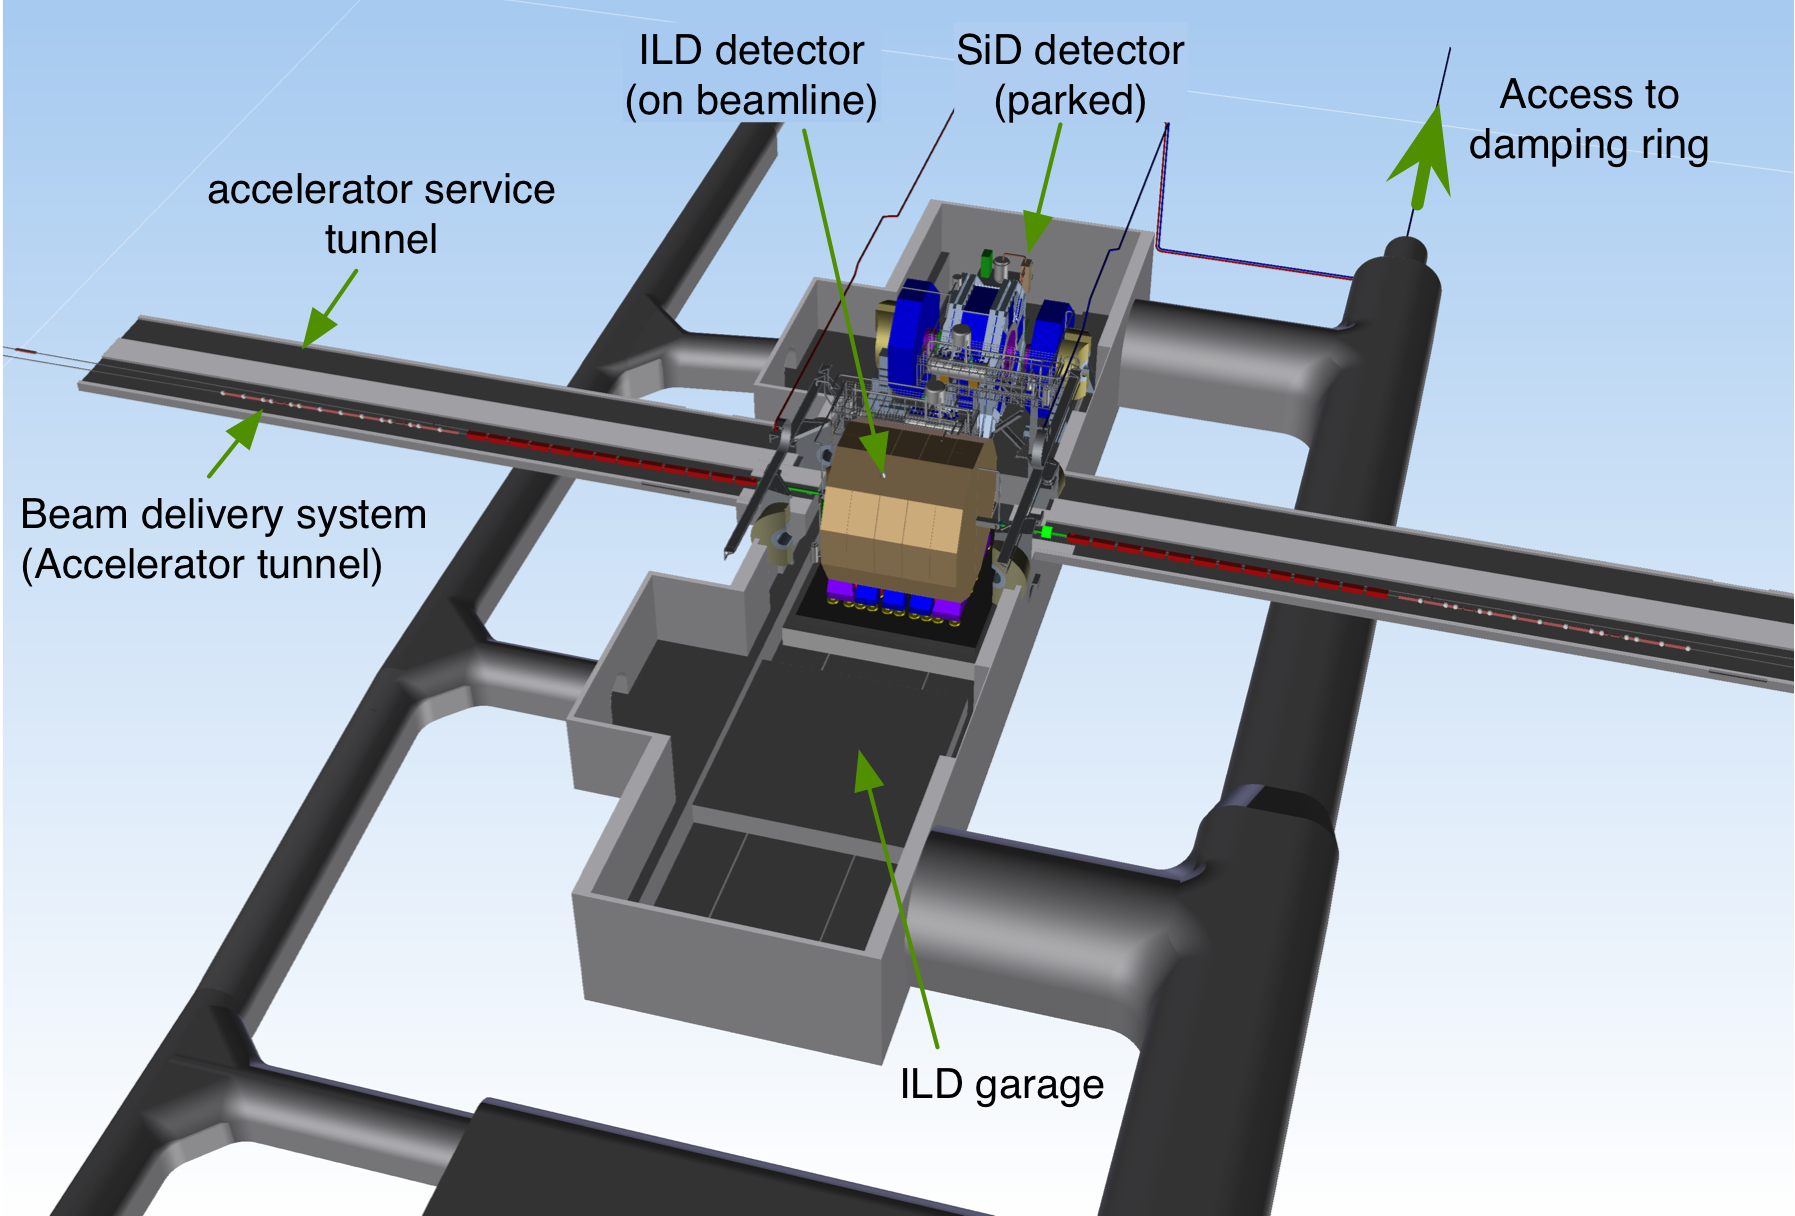
\includegraphics[scale=0.8]{./figures/ILC_detector_hall.jpg}
      \caption{Salle des d\'etecteurs de l'ILC et illustration du syst\`eme \textit{push-pull}. L'ILD est en faisceau alors que le SiD est rang\'e dans son emplacement hors faisceau.}
      \label{fig:ILC_hall}
    \end{center}
  \end{figure}
  
  Les d\'eplacements du d\'etecteurs et le syst\`eme de support sont con\c{c}us pour une centaine d'échanges en pr\'eservant les composantes des d\'etecteurs et en assurant un positionnement de pr\'ecision. L'alignement des d\'etecteurs doit \^etre effectu\'e apr\`es chaque d\'eplacement. Les d\'etecteurs seront plac\'es sur des plate-formes qui pr\'eserveront au maximum l'alignement du d\'etecteur et distribueront la charge uniform\'ement dans le sol.
  
  \medskip
  
  Malgr\'e l'importance de la pr\'esence de deux d\'etecteurs, fournissant des mesures compl\'ementaires, pour des questions de co\^ut, un seul et unique d\'etecteur pourrait voir le jour. Une autre solution serait l'arriv\'ee d'un second d\'etecteur plus tard dans le programme de physique. Celui-ci pourrait alors \^etre optimis\'e pour la physique d\'ecouverte par le premier.
  
  \subsubsection{Structure temporelle du faisceau et bruits de fond machine}
  \label{sect:beamstrahlung}
  
  \`A 250 $GeV$ dans le centre de masse, la structure en temps des faisceaux de l'ILC consiste en 1312 paquets de particules formant un train de 724 $\mu s$, le tout d\'elivr\'e \`a 5 $Hz$. A l'int\'erieur du train de paquets, la s\'eparation temporelle entre deux paquets est de 552 $ns$. La figure \ref{fig:timeStructure} illustre la structure temporelle des faisceaux. Environ toute les 200 $ms$ un train de paquets est émis. Cela donne un temps mort d'environ 199 $ms$ avant r\'e-\'emission d'un train. Ce temps mort peut être utilis\'e pour diminuer la puissance consomm\'ee par les d\'etecteurs en les mettant en veille.
  
  \begin{figure}[!htb]
    \begin{center} 
      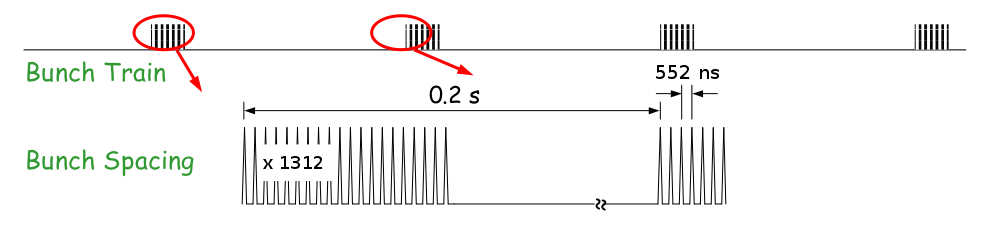
\includegraphics[scale=0.40]{./figures/bunch_structure.png}
      \caption{Structure en temps des faisceaux de l'ILC.}
      \label{fig:timeStructure}
    \end{center}
  \end{figure}  
  
  \medskip
  
  Alors qu'il est restreint au LHC, le bruit de fond machine est beaucoup plus pr\'esent \`a l'ILC (par rapport au flux de particules provenant des collisions). Ce bruit de fond est cr\'e\'e par de nombreux processus relatifs aux faisceaux de particules. Les particules de bruit de fond produites, impactent essentiellement les premiers \'el\'ements de d\'etections du fait de leur faible impulsion transverse. Parmi les principales sources de bruit de fond machine, on trouve le \textit{beamstrahlung}, le rayonnement synchrotron, les muons et les neutrons. Un nombre important de paires $e^+ e^-$ de faible \'energie est produit autour du point d'impact lors de l'interaction d'un faisceau avec l'autre ; ce processus se nomme \textit{beamstrahlung}. Lorsque deux paquets se croisent au niveau de la r\'egion d'interaction, les \'electrons (positons) sont perturb\'es par le champ \'electrique de l'autre paquet. Les électrons (positons) sont alors d\'evi\'es et ils produisent du rayonnement synchrotron. Cet effet \`a l'avantage de compresser les paquets et donc d'augmenter la luminosit\'e. Cependant le rayonnement \'emis d\'egrade la r\'esolution en \'energie des particules. L'\'etat initial est alors connu avec moins de pr\'ecision. Les photons \'emis par bremstrahlung suivent la direction du faisceau. Ils ne sont donc pas une source majeur de bruit de fond. Cependant, les photons produits, s'ils sont assez \'energ\'etiques, peuvent interagir et cr\'eer des paires \'electron-positon.
 
  \medskip
  
  Plusieurs cas de figure se pr\'esentent, les cr\'eations de paires coh\'erentes et incoh\'erentes. La cr\'eation de paires coh\'erentes \cite{Chen:1989fd} est un processus similaire \`a la cr\'eation de paires qui s'\'etablie lorsque un photon interagit avec le champ \'electromagn\'etique d'un noyau. Cette fois-ci c'est le champ \'electromagn\'etique des paquets qui induit la cr\'eation de paires. Ce processus est estim\'e n\'egligeable \`a l'ILC. Cependant, la cr\'eation de paires incoh\'erentes \cite{Zolotorev:1987wk}, n'est elle, pas n\'egligeable. Des processus de diffusions des photons provenant des deux paquets se rapprochant entrent en jeu. Trois processus majoritaires sont responsable de la cr\'eation de paires incoh\'erentes. Si le deux photons sont virtuels, le processus de \textit{Landau-Lifshitz} entre en jeu. Ce processus est responsable d'environ $1/3$ de la production de paires incoh\'erentes. Lorsqu'un photon est r\'eel et l'autre virtuel, le processus de \textit{Bethe-Heitler} donne naissance \`a environ $2/3$ de la production de paires incoh\'erentes. Enfin, lorsque les deux photons sont r\'eels, le processus de \textit{Breit-Wheeler} produit environ $1\%$ des paires incoh\'erentes. 
  
  \begin{figure}[!htb]
    \begin{center} 
      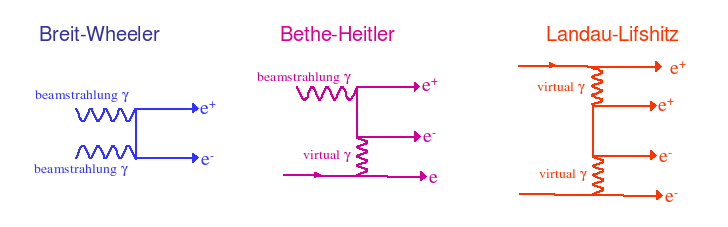
\includegraphics[scale=0.60]{./figures/beamstrahlung_processes.png}
      \caption{Diff\'erents processus participant \`a la cr\'eation de paires \'electron-positon incoh\'erentes \cite{Zolotorev:1987wk} \`a l'ILC.}
      \label{fig:beamstrahlung_processes}
    \end{center}
  \end{figure}
  
  \medskip
  
  La figure \ref{fig:beamstrahlung_processes} illustre les diagrammes de \textit{Feynman} de ces processus. Les particules ainsi cr\'e\'ees, induisent des impacts sur les premi\`eres couches de d\'etection. Du fait du fort champ magn\'etique et de leur relativement faible impulsion, ces particules peuvent boucler et cr\'eer d'autres impacts. De plus, ces particules peuvent aussi \^etre r\'etro-diffus\'ees depuis les r\'egions tr\`es \`a l'avant, au niveau des calorim\`etres de faisceau. Cela augmente de nouveau le nombre d'impacts.
  
  \medskip
  
  Concernant les autres sources de bruits machine, on notera qu'un syst\`eme de collimateurs est employ\'e afin de réduire le bruit g\'en\'er\'e par le rayonnement synchrotron produit lors du croisement des paquets. D'autres techniques sont employ\'ees pour r\'eduire l'impact du bruit de fond compos\'e de muons et de neutrons. Les muons sont produits lors de l'interaction du faisceau avec les collimateurs, et les neutrons sont le r\'esultat de l'interaction des \'electrons et positons cr\'e\'es par beamstrahlung ou issus d'un faisceau mal focalis\'e avec la ligne de faisceau ou les d\'etecteurs crois\'es. D'autres neutrons peuvent \^etre r\'etro-diffus\'es depuis les absorbeurs de faisceau en fin de ligne. Ce type de bruit de fond est rare et on peut le consid\'erer n\'egligeable en premi\`ere approximation.
  
  \medskip
  
  Pour se d\'efaire du \textit{beamstrahlung}, un dipôle a \'et\'e ajout\'e afin de guider les particules charg\'ees produites \`a l'ext\'erieur du d\'etecteur. Ce dipôle cr\'ee un champ magn\'etique nomm\'e champ \textit{anti-DID}. Cependant, malgr\'e ce champ, le d\'etecteur de vertex sera toujours affect\'e par le bruit de fond. Une \'etude sur le taux d'occupation des premi\`eres couches de d\'etection induit par la production de paires incoh\'erentes a \'et\'e r\'ealis\'ee par le groupe \textit{PICSEL} \cite{2009arXiv0902.2707D}. De nouvelles \'etudes ont \'et\'e men\'ees dans le cadre du \textit{TDR}. Ces nouvelles valeurs sont list\'ees en figure \ref{fig:tx_occupation} \cite{Vogel:2008zza}.
  
  \begin{figure}[!htb]
    \begin{center} 
      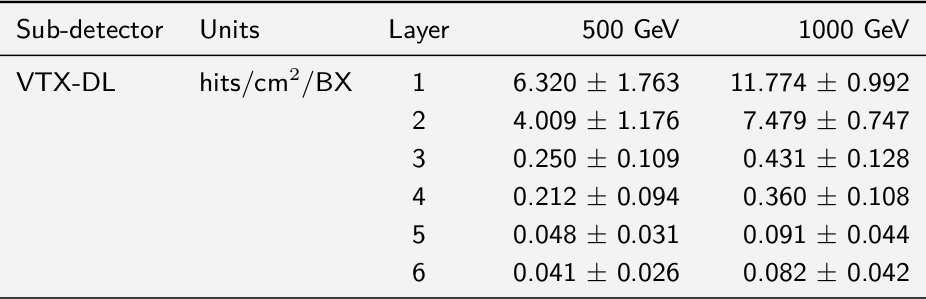
\includegraphics[scale=0.40]{./figures/table_beamstrahlung.png}
      \caption{Densit\'e d'impacts par unit\'e de surface et par croisement de faisceau pr\'evu \`a l'ILD.}
      \label{fig:tx_occupation}
    \end{center}
  \end{figure}
  
  \medskip
  
  On notera la valeur de $6.3 \pm 0.8$ impacts par $cm^2$ et par croisement de faisceaux (1 croisement de faisceaux = 1 BX) pour la premi\`ere couche du détecteur de vertex avec une \'energie de 500 $GeV$ dans le centre de masse. \`A partir de la troisi\`eme couche ce taux baisse \`a moins de $0.5$ impacts par $cm^2$ et par croisement de paquet. Toutefois on gardera \`a l'esprit que ces valeurs ne sont que des estimations et non des mesures. Une nouvelle \'etude d\'etaill\'ee de ce bruit de fond sur le d\'etecteur de vertex a \'et\'e r\'ealis\'ee au cours de cette th\`ese. Elle conduit notamment \`a une nouvelle estimation des temps de lecture des capteurs utilis\'es pour le d\'etecteur de vertex. Nous reviendrons sur ces valeurs dans le chapitre \ref{chap:alignement} portant sur l'alignement des \'echelles et le bruit de fond de faisceau.
  
  \medskip

  Ainsi, le beamstrahlung impose une certaine tenue aux radiations pour les d\'etecteurs situ\'es proches du point d'interaction. En effet, en terme de radiations, \'etant donn\'e la faible section efficace $e^+$ $e^-$ pour les \'ev\'enements que l'on veut \'etudier \`a l'ILC, le nombre d'impacts dans la premi\`ere couche du d\'etecteur de vertex par croisement de faisceau et par $cm^2$ est n\'egligeable par rapport au \textit{beamstrahlung}. En prenant la section efficace totale $e^+$ $e^-$, un calcul approch\'e rapide nous donne un nombre moyen de particules produites par croisement de faisceau et par $cm^2$ de : $N = L \times \sigma_{tot} / (5 \times BXs \times 2\pi R Z) \lesssim 2 \times 10^{-5} $ Avec R=$16 \, mm$, $Z = 62.5 \, mm$, $L = 2 \times 10^{34} \, cm^{-2}s^{-1}$, 5 le taux de r\'ep\'etition (= nombre de trains par seconde) de la machine et $BXs$ le nombre de croisements de paquets par train. Le taux d'occupation des premi\`eres couches du d\'etecteur de vertex est alors totalement domin\'e par le beamstrahlung. Ce dernier constitue une contrainte sur les capteurs qui seront utilis\'es pour \'equiper les premi\`eres couches de d\'etection. Les détails de l'optimisation du d\'etecteur de vertex \'equip\'e de capteurs CMOS, imagin\'e par le groupe $PICSEL$ de l'IPHC pour \'equiper l'ILD, sera d\'ecrit dans le prochain chapitre.
  
  \medskip
  
  Nous allons \`a pr\'esent d\'ecrire les d\'etecteurs de l'ILD.
  
%   \subsubsection{Principaux d\'eveloppements pour les d\'etecteurs}
%   
%   Depuis quelques ann\'ees, d'importants programmes internationaux de recherche et développement visent à d\'evelopper les futurs d\'etecteurs de l'ILC. Ils ont comme objectifs principaux le d\'eveloppement des calorim\`etres, des syst\`emes de trajectom\'etrie, et des d\'etecteurs de vertex. Étant donn\'e que de nombreux canaux de physique entraînent la cr\'eation de multi-jets, les syst\`emes de calorim\'etrie doivent assurer une bonne identification de ceux-ci. Ainsi, une s\'eparation nette des jets, avec une reconstruction de la masse invariante des di-jets, est essentielle. Le PFA permettra d'atteindre des r\'esolutions sans pr\'ec\'edent et sera utilis\'e pour les d\'etecteurs de l'ILC. Le PFA fonctionne de la fa\c{c}on suivante. Tout d'abord le quadri-vecteur énergie-impulsion de toutes les particules visibles est reconstruit, puis dans un second temps, la reconstruction du jet est effectu\'ee. Pour les particules charg\'ees, la mesure de ce quadri-vecteur est effectu\'ee par le d\'etecteur de traces (\textit{tracker}). En effet, pour ces particules la pr\'ecision est meilleure que celle obtenue par le calorim\`etre. Les photons et les hadrons neutres seront mesur\'es dans les calorim\`etres \'electromagn\'etiques (photons) et hadroniques (hadrons neutres). Cela requi\`ere une bonne s\'eparation de toutes les particules qui interagissent avec le calorim\`etre. En pratique, cette s\'eparation est difficile et la résolution en \'energie en est affect\'ee. Pour permettre d'obtenir une bonne distinction des particules, le calorim\`etre doit poss\'eder une grande granularit\'e tant longitudinale que transverse.
  
%    La r\'esolution sur la masse invariante est d\'efinie par une pr\'ecision sur les largeurs des bosons de jauges d'environ 3$\%$
  
%   \medskip
%   
%   De nouvelles technologies ont \'et\'e explor\'ees pour la calorim\'etrie. Pour le calorim\`etre hadronique (HCAL) de nombreuses technologies se basant sur des absorbeurs en tungst\`ene ou en acier ont \'et\'e \'etudi\'ees. Parmi celles-ci ce trouvent les photo-multiplicateurs au silicium (SiPM), les MAPS (Monolithic active pixel sensors) et les d\'etecteurs gazeux comme les RPCs (Resistive Plate Chambers) ou les Micromegas. Un vaste effort de R$\&$D a \'et\'e accompli afin de tester ces solutions, de valider les simulations de celles-ci et de tester les performances du PFA. Ces développements ont principalement \'et\'e r\'ealis\'es par la collaboration CALICE. Par exemple, un calorim\`etre hadronique digital \'equipé de GRPCs et contenant environ 500 000 canaux a déjà \'et\'e test\'e. Un \'ev\`enement enregistr\'e par ce prototype est visible en figure \ref{fig:HCAL_event}.
%   
%   \begin{figure}[!htb]
%     \begin{center}
%       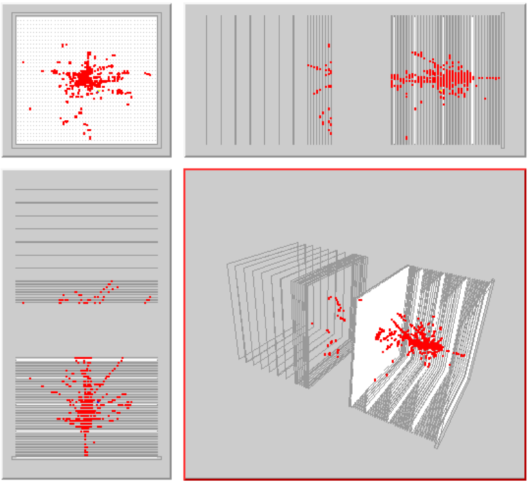
\includegraphics[scale=1.0]{./figures/DHCAL-ED.pdf}
%       \caption{Affichage d'un \'ev\`enement montrant le passage d'un pion de 10 GeV dans le détecteur DHCAL, \'equip\'e de GRPCs}
%       \label{fig:HCAL_event}
%     \end{center}
%   \end{figure}
% 
%   \medskip
%   
%   Le calorim\`etre \'electromagn\'etique doit identifier les photons et mesurer leur \'energie. Il doit pouvoir s\'eparer un photon d'un autre photon proche ou d'un hadron proche pour la reconstruction du jet gr\^ace au PFA. Pour les absorbeurs, le tungst\`ene constitue un bon choix puisque sa longueur de radiation (X0) \'electromagn\'etique et sa longueur d'interaction nucl\'eaire ($\lambda$) sont tr\`es diff\'erentes. Le tungst\`ene poss\`ede de plus un faible rayon de Moli\`ere, ce qui minimise l'\'etendue transverse des gerbes \'electromagn\'etiques. Les technologies au silicium (matrices de diodes en silicium ou MAPS) offrent la plus grande compacit\'e (et le plus grand rayon de Moli\`ere effectif) avec une stabilit\'e de calibration excellente. Les pistes scintillatrices avec des photo-détecteurs en silicium ont une segmentation effective \'equivalente pour un co\^ut plus r\'eduit, mais sont moins compactes. Ces options peuvent aussi \^etre combin\'ees pour former un syst\`eme hybride.
%   
%   \medskip
%   
%   Les d\'eveloppements du côt\'e de la trajectom\'etrie se sont orient\'es vers les technologies bas\'ees sur le silicium et les d\'etecteurs gazeux. Du côt\'e des technologies bas\'ees sur le silicium on trouve les \textit{strips} et les capteurs hautement pixelis\'es. Pour les detecteurs gazeux, la d\'etection sera r\'ealis\'ee grâce \`a une chambre \`a projection temporelle (TPC). Pour collecter les charges produites par celle-ci les développements s'orientent vers les \textit{Micromegas}, les \textit{GEM} ou les capteurs CMOS.
%   
%   \medskip
%   
%   La d\'etection et l'identification des fermions lourds reposent sur la reconstruction des vertex d\'eplac\'es. Cette reconstruction est elle m\^eme reli\'ee \`a la r\'esolution du d\'etecteur de vertex proche du point d'interaction. Un d\'etecteur de vertex dot\'e d'un faible pas inter-pixel et d'un budget de mati\`ere le plus r\'eduit possible, le tout proche du point d'interaction est recquit. La premi\`ere couche de capteurs du d\'etecteur de vertex pourra \^etre plac\'ee \`a une distance de 14 \`a 16 $mm$ du point d'interaction. Le budget de mati\`ere de ce d\'etecteur de vertex devra \^etre de l'ordre de 0.1 $\%$ $X_0$ par couche ; et celui pour un détecteur de trace (\textit{tracker}) en silicium devra \^etre de moins de 1 $\%$ $X_0$ par couche. Pour une TPC, le budget de mati\`ere est accumul\'ee dans les extr\'emités (d\'etection des charges) et un budget de mati\`ere d'environ 30 $\%$ $X_0$ pour les extr\'emit\'es est l'objectif \`a atteindre.
%   
% %   et des leptons $\tau$
%   
%   \medskip
%   
%   Afin de réduire la puissance dissip\'ee globale du d\'etecteur, les d\'etecteurs peuvent \^etre mis en veille durant 199 $ms$ toute les 200 $ms$, c'est ce que l'on appelle le \textit{power-pulsing}. Cela entraîne une baisse de la puissance consomm\'ee par les d\'etecteurs d'un facteur proche de 100. De ce fait, les d\'etecteurs de vertex et de traces n'ont pas besoin de refroidissement actif, ce qui m\`ene \`a une réduction significative du budget de mati\`ere. Ainsi un simple refroidissement par pulsation d'air \`a l'intérieur des cylindres du d\'etecteur de vertex permet de dissiper les environ 20 W consomm\'es.
%   
%   \medskip
%   
%   Nous allons \`a pr\'esent nous focaliser sur l'ILD. Ce dernier \'etant le d\'etecteur pour le lequel le groupe \textit{PICSEL} \'etudie un d\'etecteur de vertex.
  
  \subsubsection{ILD}
  
  L'ILD est un d\'etecteur polyvalent optimis\'e pour le PFA. Il est constitu\'e d'un d\'etecteur de vertex de haute pr\'ecision, suivi par un syst\`eme de trajectom\'etrie hybride r\'ealis\'e \`a partir d'une combinaison de plans de micropistes et d'une TPC, le tout suivi d'un système de calorim\'etrie. Tous ces \'el\'ements sont plac\'es dans un champ magn\'etique de 3.5 T d\'elivr\'e par un sol\'eno\"ide. Le sol\'eno\"ide est plac\'e à la suite des calorim\`etres afin d'optimiser les associations entre les traces et les d\'ep\^ots d'\'energie dans les calorim\`etres. \`A l'ext\'erieur du sol\'eno\"ide, la culasse est \'equip\'ee avec un d\'etecteur de muons réalisant aussi la calorim\'etrie des longues gerbes. Le rayon de l'ILD mesure 783 cm pour une longueur de 1324 cm. L'ILD est illustr\'e en figure \ref{fig:ILDschema}. Les d\'etecteurs de l'ILD sont sch\'ematis\'es en figure \ref{fig:detector_ILD}.
  
  \begin{figure}[!htb]
    \begin{center} 
      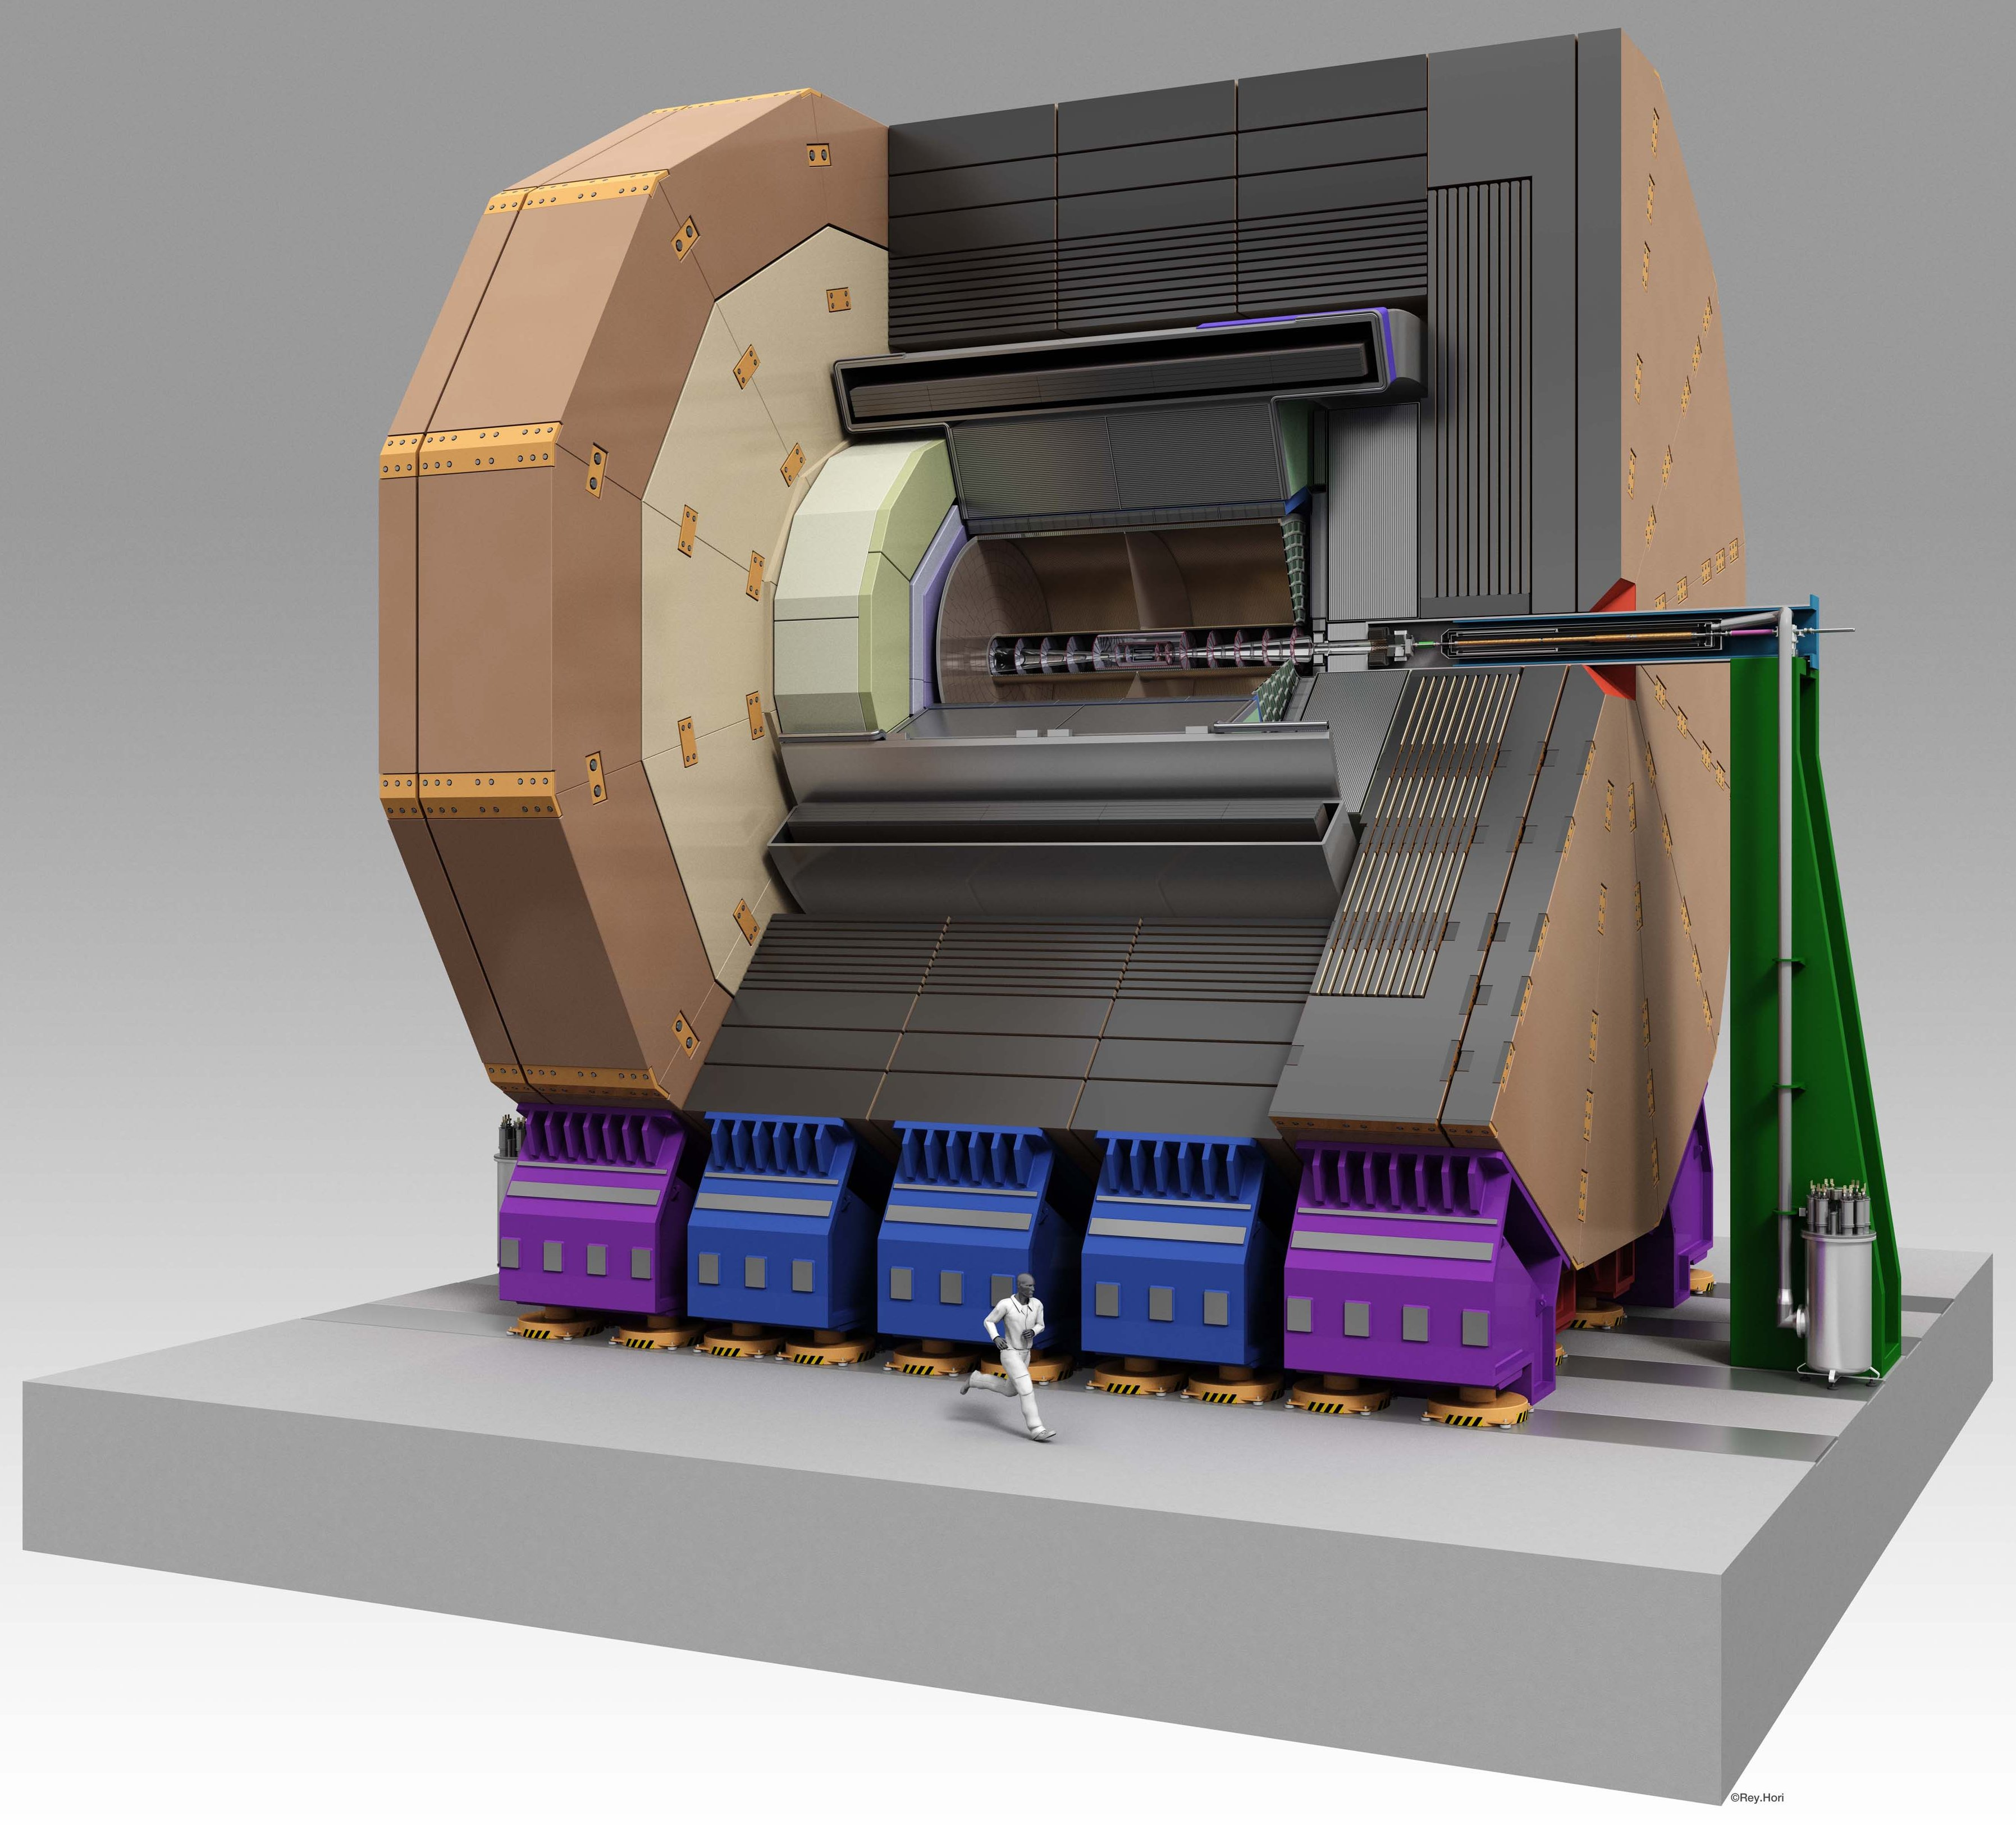
\includegraphics[scale=0.12]{./figures/ILD_schema_global.jpg}
      \caption{Sch\'ema de l'ILD.}
      \label{fig:ILDschema}
    \end{center}
  \end{figure}

  \medskip
  
  Le d\'etecteur de vertex de l'ILD (VTX) sera compos\'e de 3 super-couches double face. Une seconde option consiste à \'equiper ce d\'etecteur de vertex de 5 couches simple face. Ces couches seront "cylindriques" avec des rayons variant de 16 \`a 60 mm. La longueur (selon Z) de la premi\`ere super-couche mesurera la moiti\'e des deux autres afin de minimiser l'impact du bruit de fond machine. La technologie dans laquelle sera con\c{c}ue le VTX n'a pas encore \'et\'e choisie. Cependant, le VTX est optimis\'e pour une bonne r\'esolution spatiale alli\'ee \`a un budget de mati\`ere r\'eduit. Nous reviendrons dans le prochain chapitre sur les caract\'eristiques de ce d\'etecteur de vertex puisqu'il s'agit du d\'etecteur dont il est question dans cette th\`ese. 
  %Nous rappelons que l'objectif de cette th\`ese est l'\'etude de la valeur ajout\'ee des \'echelles double face en terme d'alignement.
%   Nous verrons comment r\'ealiser l'alignement d'\'echelles double faces d'une m\^eme couche, selon leur zone de recouvrement, \`a l'aide de mini-vecteurs pouvant \^etre reconstruits \`a partir des coups pr\'esents sur chaque face d'une \'echelle.

  \medskip
  
  \`A la suite du d\'etecteur de vertex, se trouve un système de trajectom\'etrie interm\'ediaire compos\'e de détecteurs bas\'e sur des plans de micropistes ou des pixels au silicium. Dans la partie centrale de celui-ci, deux couches de d\'etecteurs compos\'es de \textit{strip} sont interpos\'es entre le VTX et la TPC (SIT). Dans la r\'egion avant, un syst\`eme de deux disques compos\'es de pixels et 5 disques compos\'es de \textit{strip} (FTD) offre un recouvrement pour les petits angles. Une des principales caract\'eristiques de l'ILD est sa TPC de grand volume, permettant de d\'etecter jusqu'\`a 224 points par trace. Cette TPC est optimis\'ee pour sa résolution spatiale en 3 dimensions. Elle participe \`a l'identification des particules par la m\'ethode du $dE/dx$. \`A l'ext\'erieur de la TPC se trouve un syst\`eme de trajectom\'etrie secondaire compos\'e de \textit{strips} qui permet l'am\'elioration de la reconstruction des traces et offre une redondance entre la TPC et les calorim\`etres. Ce syst\`eme est compos\'e de deux d\'etecteurs. L'un est constitu\'e d'une couche de d\'etecteur et si\`ege derrière les parties avant de la TPC (ETD) et l'autre se trouve entre la TPC et le calorim\`etre \'electromagn\'etique (SET).
  
  \medskip
  
    \begin{figure}[htb!]
     \begin{center}
        \subfigure[Vue en coupe des d\'etecteurs de l'ILD.]{
            \label{fig:ILD_coupe}
            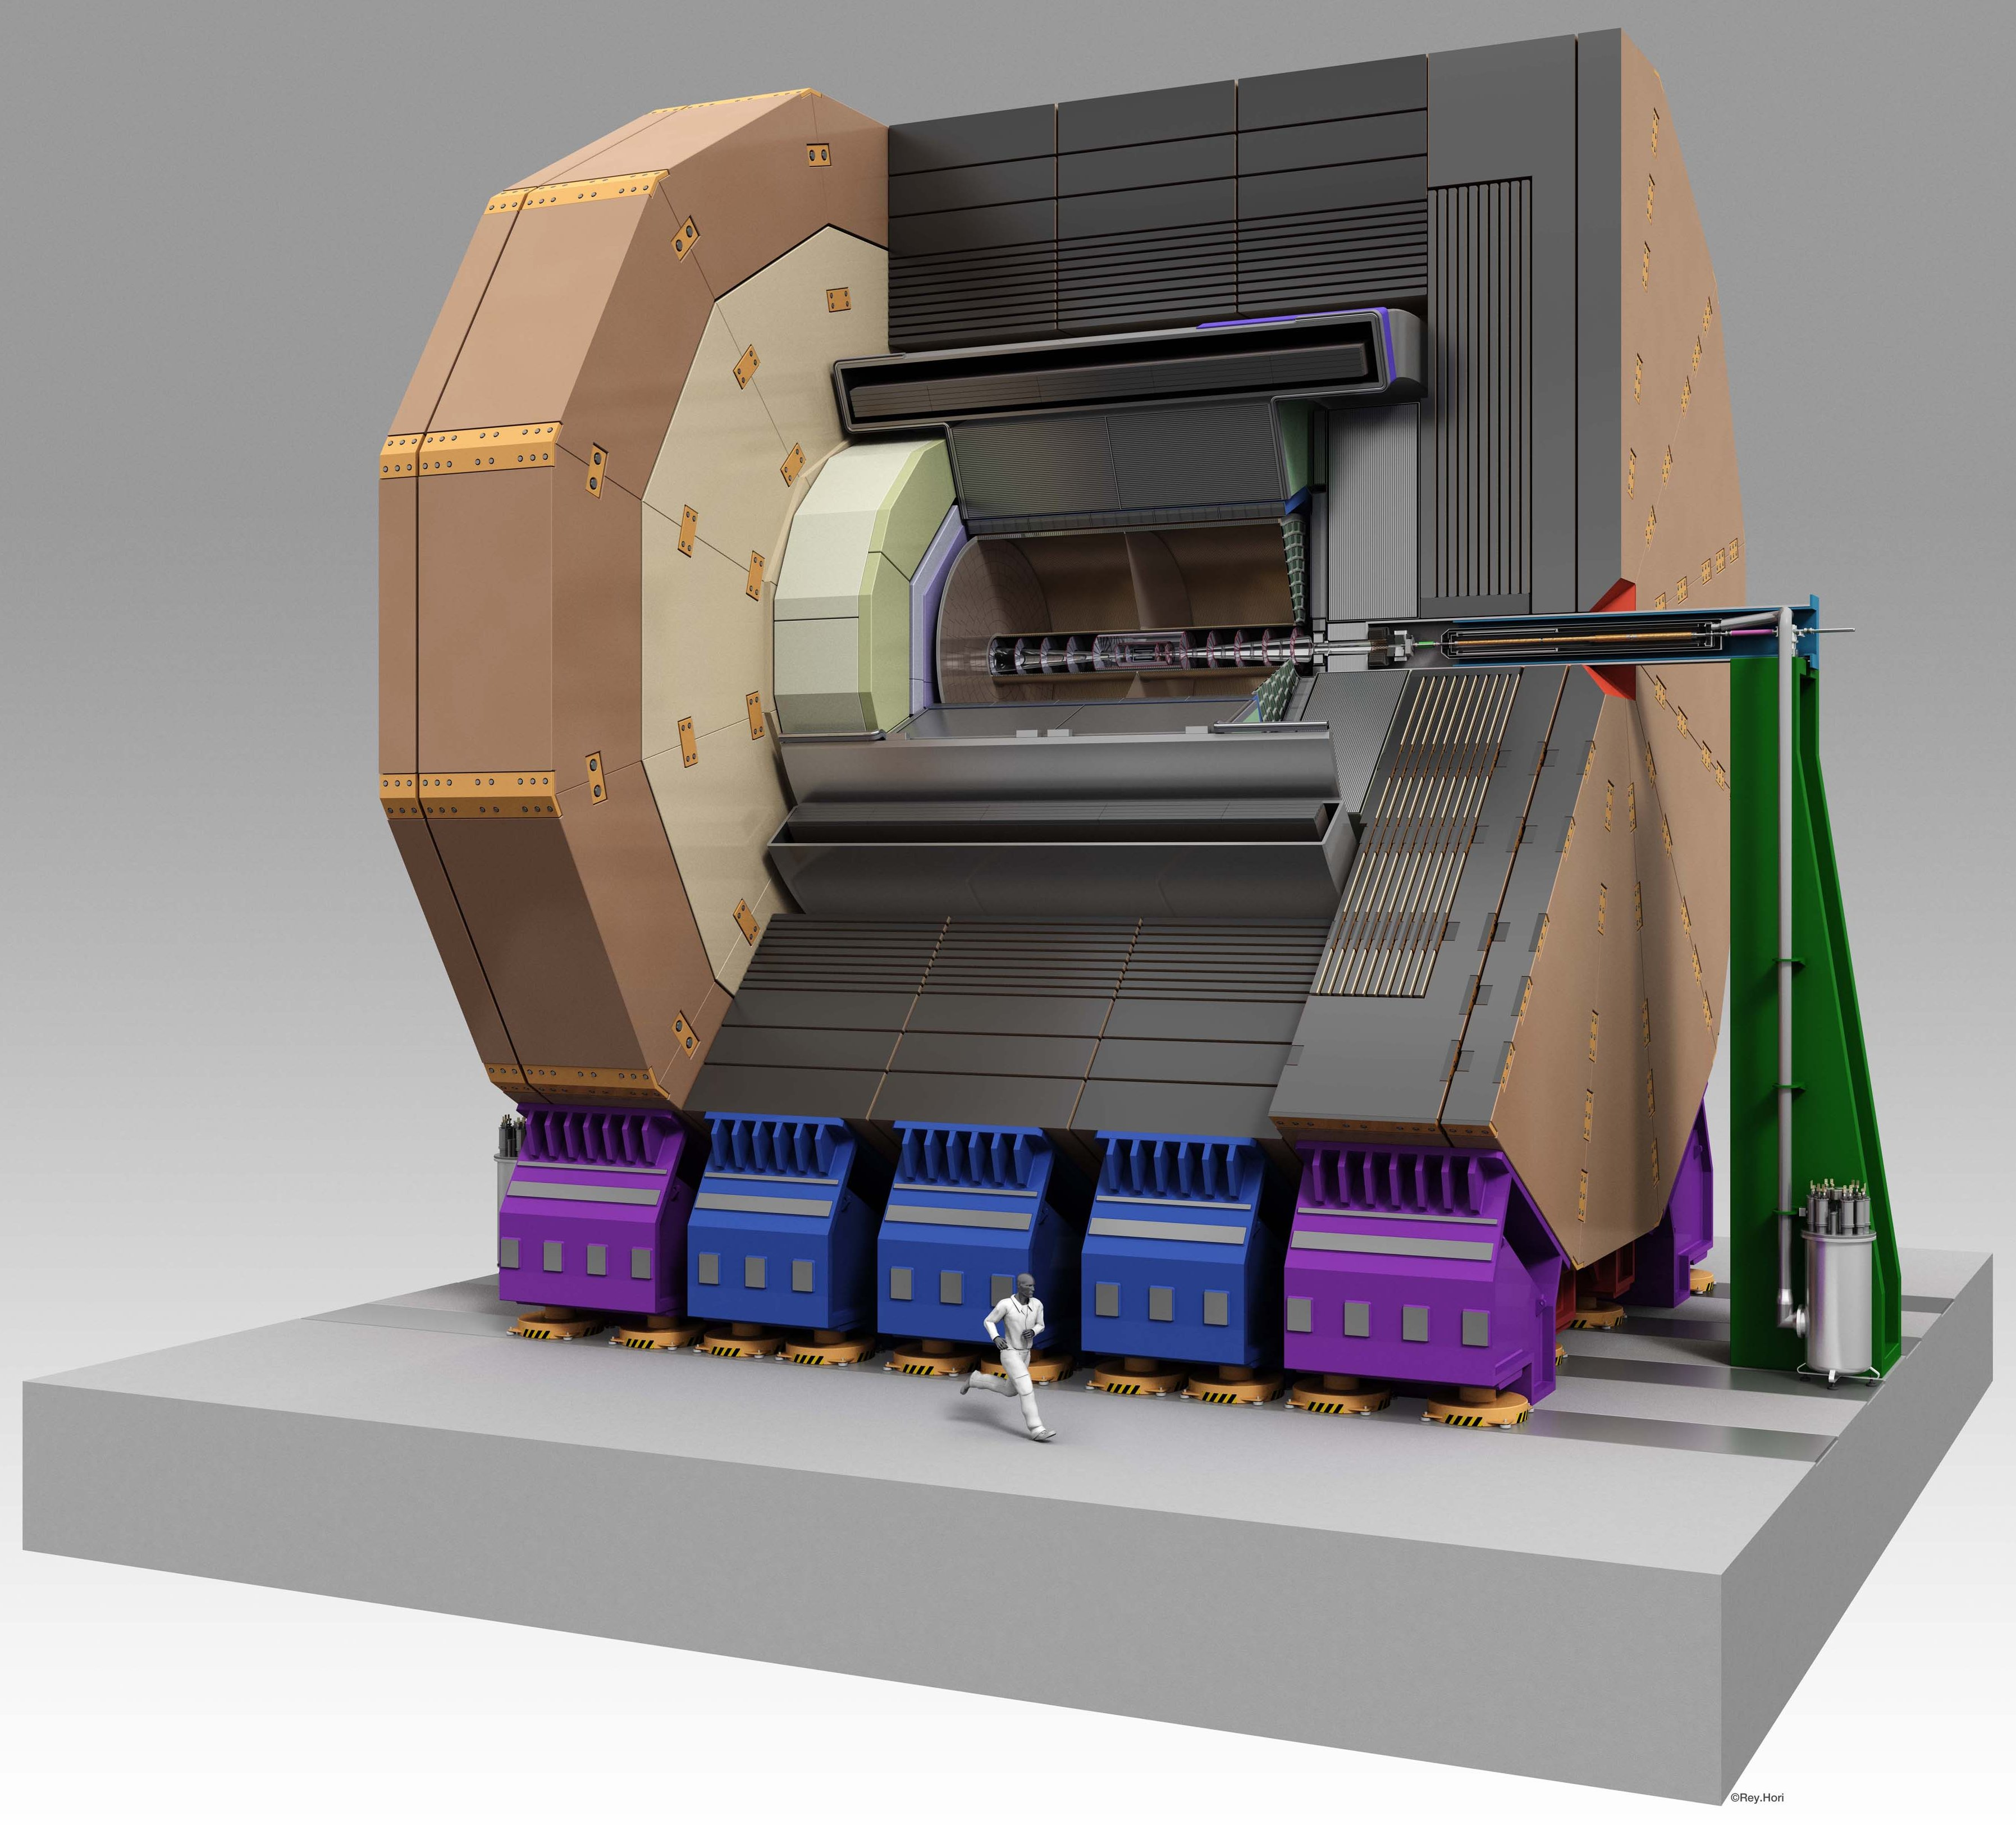
\includegraphics[width=0.47\textwidth]{./figures/ILD_schema_global.jpg}
        }
        \subfigure[Zoom sur les syst\`emes de tracking.]{
           \label{fig:ILD_Zoom_Tracker}
           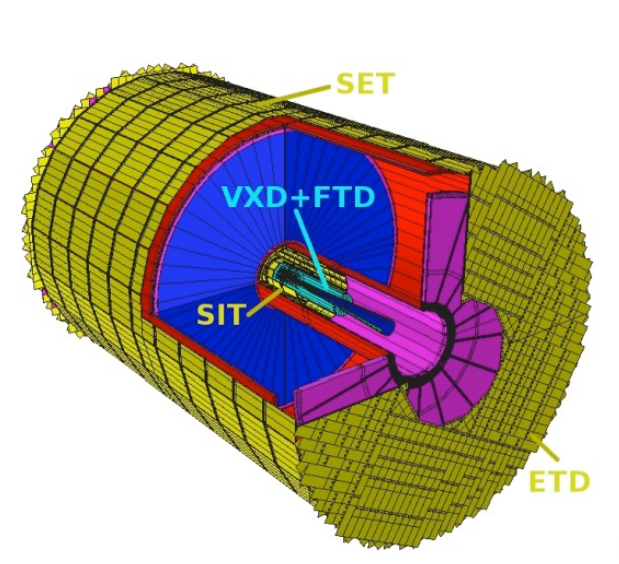
\includegraphics[width=0.47\textwidth]{./figures/ILD_SIT_FTD_SET_ETD.png}
        }
     \end{center}
     \caption{Vues sch\'ematiques de l'ILD.}
     \label{fig:detector_ILD}
   \end{figure}
  
  Le calorim\`etre \'electromagn\'etique (ECAL) est hautement granulaire et fournit jusqu'\`a 30 points de mesure en profondeur. Il devrait fournir des cellules de $5 \times 5 \, mm^2$ selon sa dimension longitudinale. L'ECAL est d\'ecoup\'e en deux parties majeures, la partie centrale et cylindrique et les bouchons qui ferment le calorim\`etre aux extr\'emités. Le calorim\`etre \'electromagn\'etique est compos\'e de plaques d'absorption en tungst\`ene et de couches sensibles r\'ealis\'ees avec des pistes scintillatrices, des diodes en silicium, ou une combinaison des deux. Le calorim\`etre \'electromagn\'etique est suivi d'un calorim\`etre hadronique (HCAL) compos\'e de 48 couches sensibles selon la dimension transverse et de cellules de petites tailles lontudinalement. Deux options sont en développement, toutes deux bas\'ees sur des absorbeurs en acier. La premi\`ere option est constitu\'ee de cellules de 3$\times$3 $cm^2$ avec une sortie analogique. La seconde option utilise des GRPC avec des cellules de 1$\times$1 $cm^2$ et une sortie semi-digitale, pour chaque cellule. Dans la continuation du faisceau, tr\`es \`a l'avant du d\'etecteur, se trouve un syst\`eme de calorim\`etres (LumiCAL, BeamCAL, LHCAL) charg\'e de mesurer avec pr\'ecision la luminosit\'e et la qualit\'e des interactions entre faisceaux.
  
  \medskip
  
  Les calorim\`etres de l'ILD sont entour\'es par une bobine supra-conductrice qui cr\'ee un champ magn\'etique axial de 3.5 T. Une culasse en fer, \'equip\'ee de pistes scintillatrices ou de RPCs, retourne le champ magn\'etique du sol\'eno\"ide et sert aussi de filtre \`a muons, de d\'etecteur de muons et de calorim\`etre pour les fins de gerbes. La figure \ref{fig:detector_ILD} illustre la g\'eom\'etrie de l'ILD.
  
  \medskip

  Afin de maximiser la sensibilit\'e des d\'etecteurs \`a la physique de l'ILC, les donn\'ees ne seront pas enregistr\'ees \`a la suite d'un signal de d\'eclenchement mais seront lues en continu.

%   \medskip
%   
%   Toutes les composantes cl\'ees de l'ILC ont \'et\'e \'evalu\'ees et les performances ont \'et\'e \'etudi\'ees en tests en faisceau. C'est en particulier le cas pour l'ambitieux projet de calorim\'etrie. Une premi\`ere \'etude de l'int\'egration des d\'etecteurs a \'et\'e r\'ealis\'ee. Elle inclut une revue des composantes des d\'etecteurs, de leur taille, et des structures n\'ecessaires \`a leur montage. Les proc\'edures de montage et de maintenance ont \'et\'e simul\'ees pour valider l'int\'egration de l'ILD. Des estimations des services n\'ecessaires ont \'et\'e incluses, et des contraintes r\'ealistes ont \'et\'e prises en compte pour la conception de l'ILD. Un mod\`ele d\'etaill\'e et complet du d\'etecteur dans son ensemble a \'et\'e r\'ealis\'e en utilisant des outils de conception assist\'ee par ordinateur. Celui-ci a ensuite \'et\'e compar\'e avec la simulation GEANT4 utilis\'e pour pr\'edire les performances de l'ILD.
  
  %Description du détecteur de vertex. (Schema global :  VXD vs SIT, TPC, etc, $
  %... )\\
%   
%   \subsubsection{Performances de l'ILD}
% 
%   Afin d'estimer les performances de l'ILD, celui-ci a \'et\'e mod\'elis\'e sous GEANT4. Pour cela des mod\`eles d\'etaill\'es des d\'etecteurs et des outils de reconstruction sophistiqu\'es ont \'et\'e mis en place. Les bruits de fond tels que la production de paires incoh\'erentes et les processus $\gamma \gamma \rightarrow \text{hadrons}$, pour un croisement de faisceau, ont \'et\'e pris en compte. Une fois le bruit de fond extrait, les \'ev\`enements sont envoy\'es dans le syst\`eme de reconstruction incluant la num\'erisation, la d\'etection de traces, la d\'etection des vertex et l'algorithme de \textit{particle flow} : PandoraPFA \cite{Thomson:2009rp}. Le budget de mati\`ere de chaque d\'etecteur est un param\`etre cl\'e. Le PFA requi\`ere un d\'etecteur de traces (tracker) fin afin de minimiser les interactions avant les calorim\`etres. Ces derniers sont quant \`a eux denses afin d'absorber au maximum les gerbes. Le budget de mati\`ere du tracker de l'ILD est inf\'erieur \`a 10$\%$ $X_0$ pour la partie centrale ($\theta \gtrsim 40 $ degr\'es). La figure \ref{fig:matILD} montre le budget de mati\`ere pour les premiers \'el\'ements de d\'etection de l'ILD. 
%   
%     \begin{figure}[!htb]
%     \begin{center} 
%       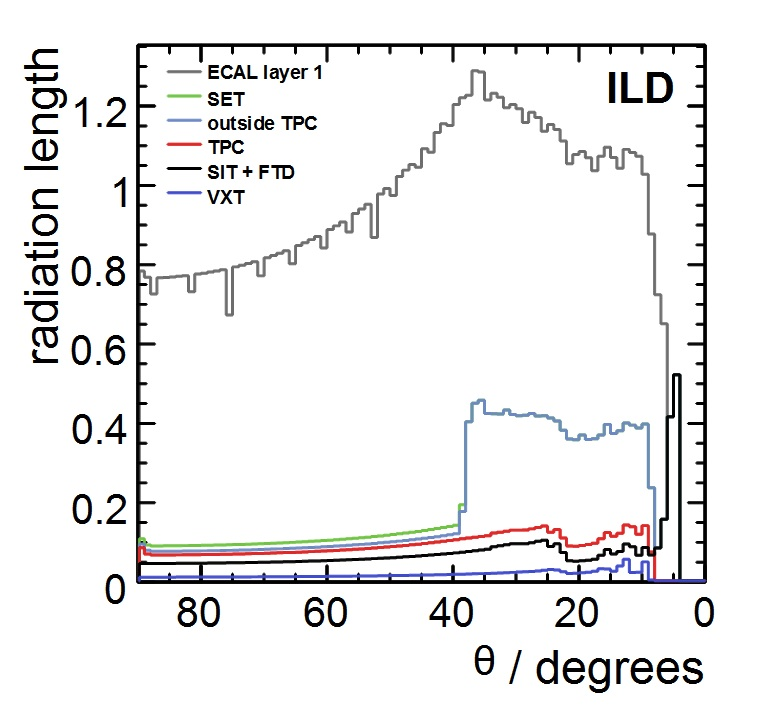
\includegraphics[scale=0.5]{./figures/material-budget_ECAL.jpg}
%       \caption{Longueur de radiation moyenne pour les premiers \'el\'ements de d\'etection de l'ILD en fonction de l'angle polaire $\theta$. La courbe rouge montre le budget de mati\`ere sans les \'el\'ements solides de la TPC. La ligne grise symbolise le budget de mati\`ere total des détecteurs, jusqu'\`a la premi\`ere couche active du calorim\`etre \'electromagn\'etique.}
%       \label{fig:matILD}
%     \end{center}
%   \end{figure}  
% 
%   \begin{figure}[!htb]
%     \begin{center} 
%       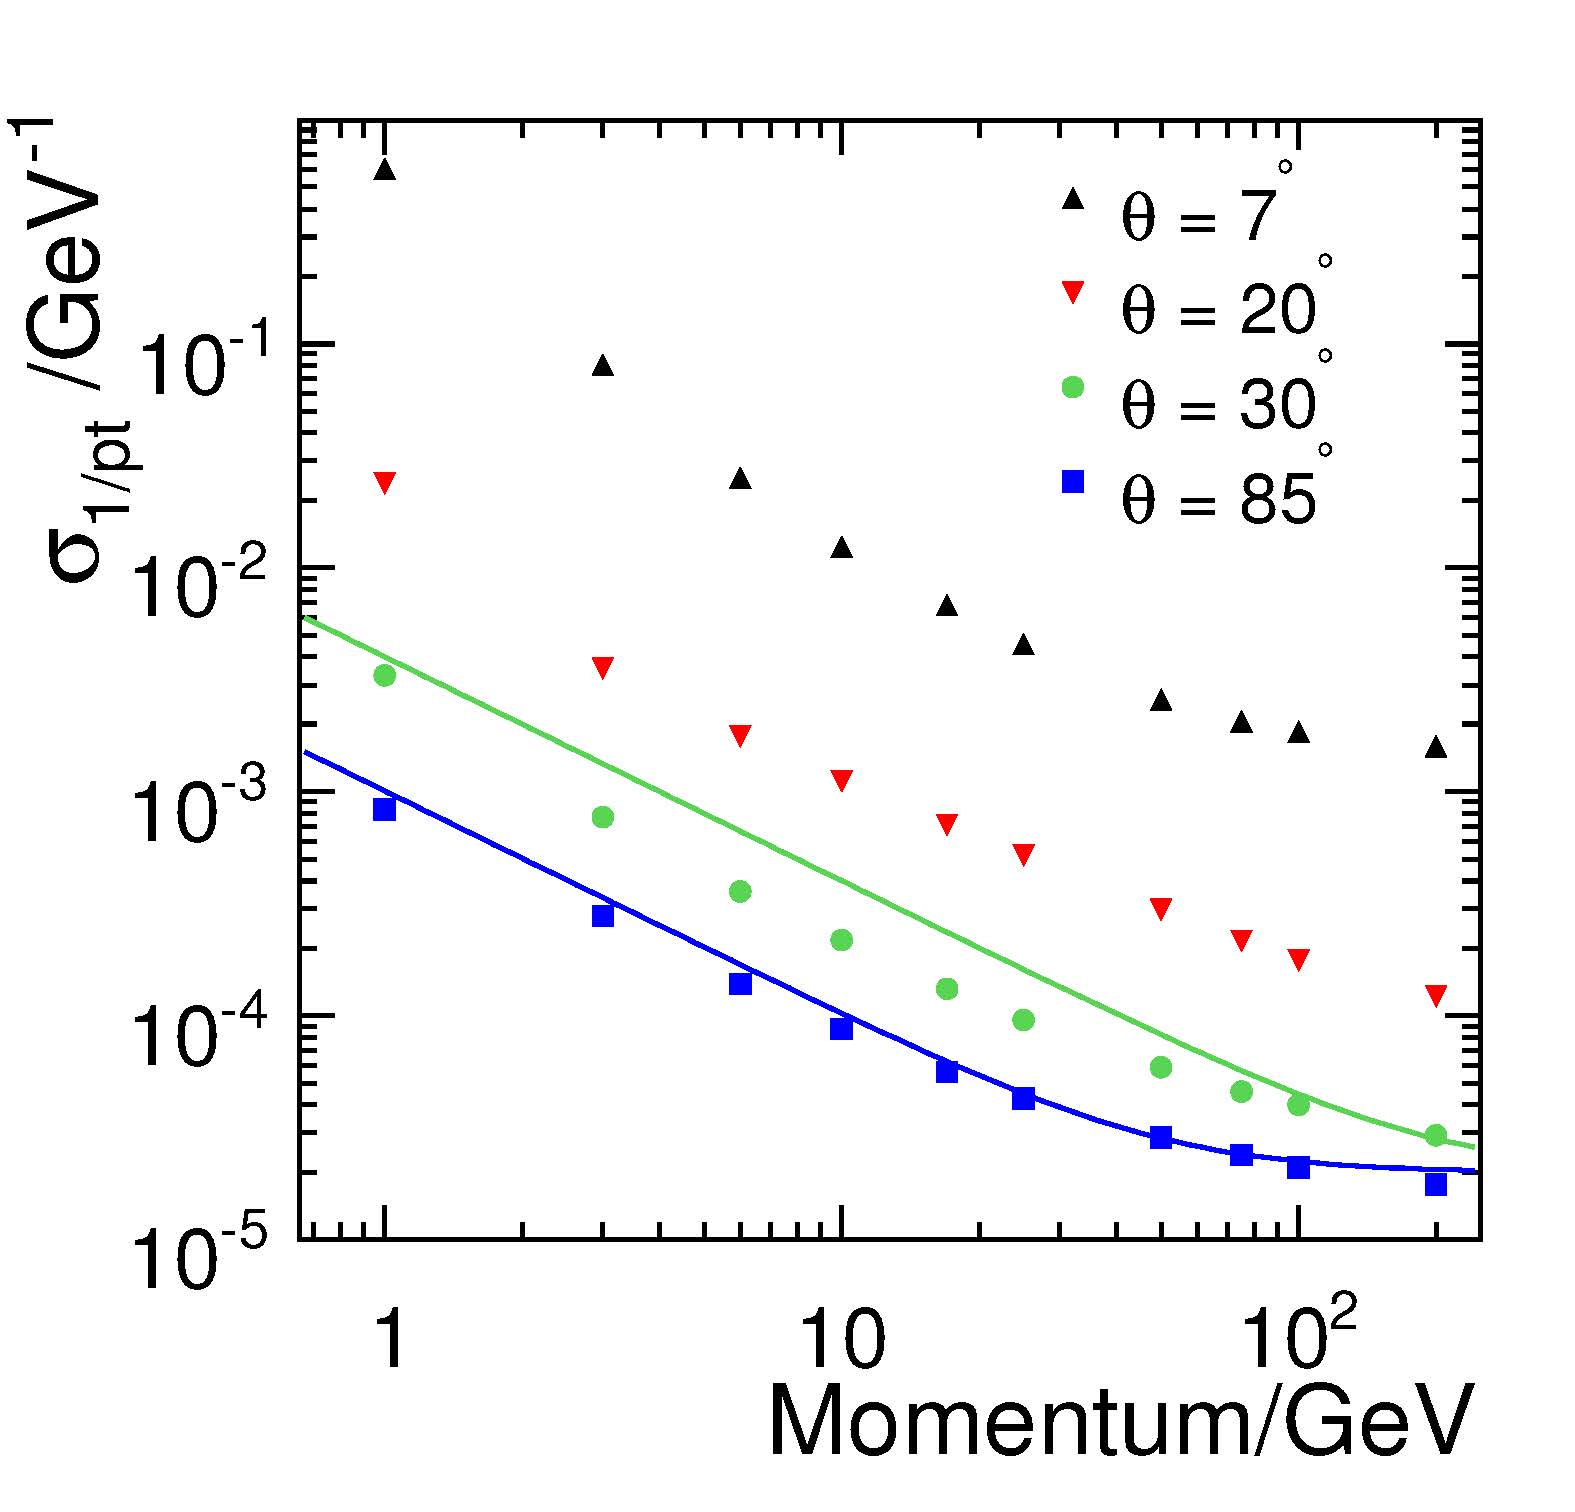
\includegraphics[scale=0.5]{./figures/deltaInvP_all_fits.jpg}
%       \caption{R\'esolution sur l'impulsion en fonction de l'impulsion transverse des particules, pour des traces d'angles polaires diff\'erents. En ligne continue les pr\'evisions th\'eoriques sont expos\'ees.}
%       \label{fig:trackingPerf}
%     \end{center}
%   \end{figure}
%   
%     \begin{figure}[!htb]
%     \begin{center} 
%       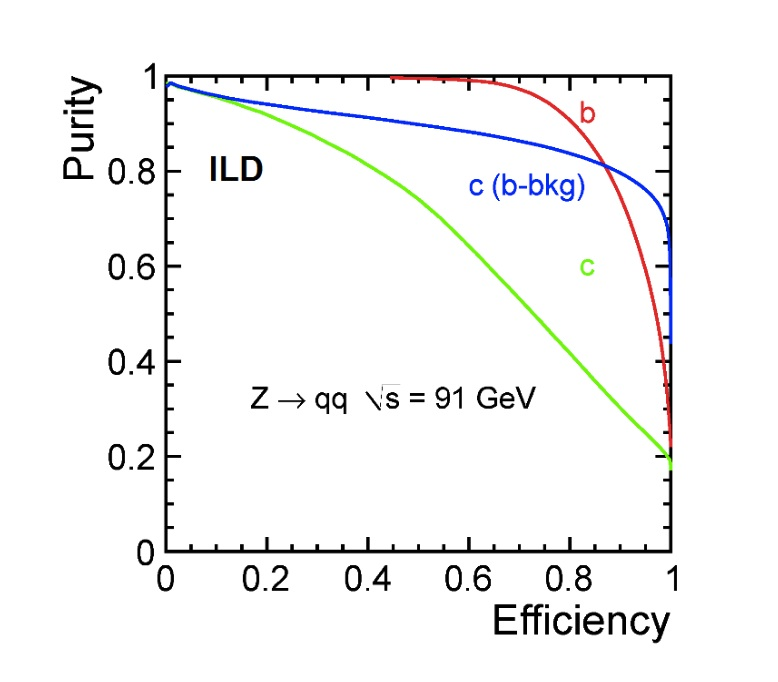
\includegraphics[scale=0.5]{./figures/evalZ-lcfiweights_qq91new_v02-test.jpg}
%       \caption{Performances de l'ILD pour l'\'etiquetage des saveurs bas\'ees sur des d\'esint\'egrations $Z \rightarrow q\overline{q}$ \`a 91 $GeV$}
%       \label{fig:displacedVertex}
%     \end{center}
%   \end{figure}
%   
%   \begin{figure}[!htb]
%     \begin{center} 
%       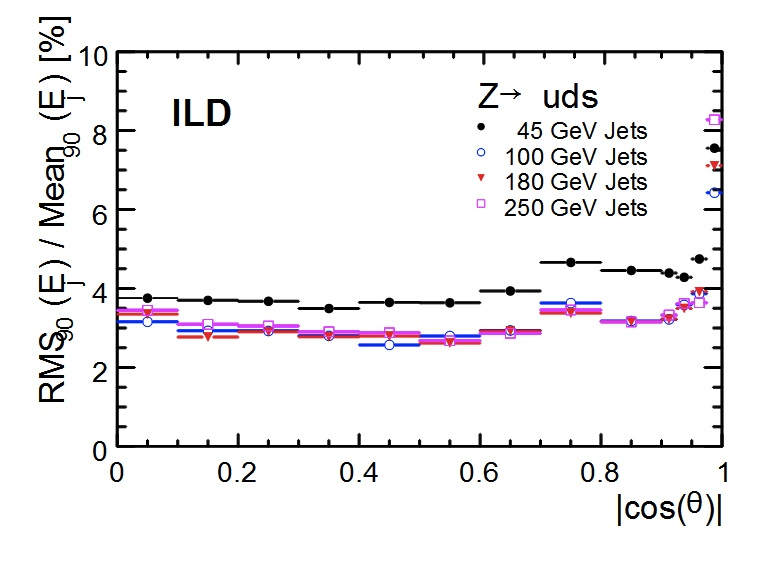
\includegraphics[scale=0.5]{./figures/ild01_o1_pflow.jpg}
%       \caption{R\'esolution sur l'\'energie (partielle) des jets \`a l'ILD en fonction de $|\cos(\theta)|$. O\`u $\theta$ est l'angle polaire \`a partir de l'axe symbolis\'e par la direction de l'\'ev\`enement.}
%       \label{fig:resoJets}
%     \end{center}
%   \end{figure}
%   
%   \medskip
%   
%   Au niveau des bouchons de l'ILD, l'augmentation du budget de mati\`ere pour la TPC est d\^ue au support de lecture de la TPC ($\theta \lesssim 40$ degr\'es). Comme cet \'el\'ement est plac\'e proche des bouchons du calorim\`etre \'electromagn\'etique, il a un impact minime sur les performances. Cela peut \^etre vu en examinant la courbe grise de la figure \ref{fig:matILD} repr\'esentant la longueur de radiation totale jusqu'\`a la premi\`ere couche active du calorim\`etre \'electromagn\'etique.
%   
%   \medskip
%   
%   Les performances simul\'ees pour la trajectom\'etrie, et pour des particules uniques, sont visibles en figure \ref{fig:trackingPerf}. La r\'esolution sur les hautes impulsions ($\approx 100 GeV/c$) \`a l'ILD devra atteindre $\sigma_{1/p_T} = 2 \times 10^{-5} (GeV/c)^{-1}$.
%   
%   \medskip
%   
%   Pour de nombreuses \'etudes, l'étiquetage des particules de longue dur\'ee de vie est primordiale. La capacit\'e \`a \'etiqueter les d\'esint\'egrations charm\'ees et belles avec une grande puret\'e a \'et\'e un objectif cl\'e dans la conception du d\'etecteur de vertex. La figure \ref{fig:displacedVertex} montre la capacit\'e de l'ILD \`a reconstruire les vertex d\'eplac\'es.
%   
%   \medskip
%   
%   La reconstruction des jets repose sur d'excellentes performances de trajectom\'etie et de calorim\'etrie, le tout combin\'e \`a des algorithmes de reconstruction sophistiqu\'es bas\'es sur le PFA. La r\'esolution obtenue permet de s\'eparer les d\'esint\'egrations des bosons W et Z. La figure \ref{fig:resoJets} illustre les r\'esolutions sur l'\'energie des jets obtenues par la simulation. Les r\'esolutions sont pr\'esent\'ees en fonction du RMS90 et de la valeur moyenne Mean90 (Ces valeurs utilisent le plus petit intervalle qui contient 90\% des événements). Cette mesure empêche de donner de l'importance aux queues des distributions d'\'energie. 
  
  \subsubsection{Détecteur de Vertex}
  \label{sect:paramVTX}
  
  Comme nous l'avons vu, lors de la pr\'esentation du programme de physique de l'ILC (voir section \ref{sect:prog_physique}), l'identification des quarks lourds (charm\'es et beaux) et des leptons tau est primordiale pour le programme de physique de l'ILC. Ainsi, la reconstruction des vertex de d\'esint\'egration des particules \`a faible dur\'ee de vie comme les m\'esons D ou B m\'erite beaucoup d'attention et demande un détecteur de vertex pr\'ecis avec un budget de mati\`ere r\'eduit. Les vertex sont reconstruits \`a partir des traces issues de la reconstruction des trajectoires des produits de d\'esint\'egration des particules \`a faible dur\'ee de vie. La reconstruction de ces trajectoires est r\'ealis\'ee gr\^ace \`a la mesure tr\`es pr\'ecise des param\`etres des traces issues des particules charg\'ees au voisinage du point d'interaction avec le d\'etecteur de vertex, combin\'ee avec les autres informations sur ces traces issues des autres syst\`emes de trajectom\'etrie. Les performances d'un syst\`eme de d\'etection de vertex peuvent \^etre exprim\'ees par la r\'esolution sur le param\`etre d'impact des particules charg\'ees. L'objectif pour le d\'etecteur de vertex de l'ILD est d'atteindre une r\'esolution sur le param\`etre d'impact $\sigma_{ip} < 5 \oplus 10/p \, \sin^{\frac{3}{2}}(\theta) \, \mu m$. La figure \ref{fig:sigmaIP} montre la résolution sur le param\`etre d'impact en fonction de l'impulsion de la particule pour deux technologies de capteurs et pour deux angles de productions diff\'erents.
  
  \begin{figure}[!htb]
    \begin{center} 
      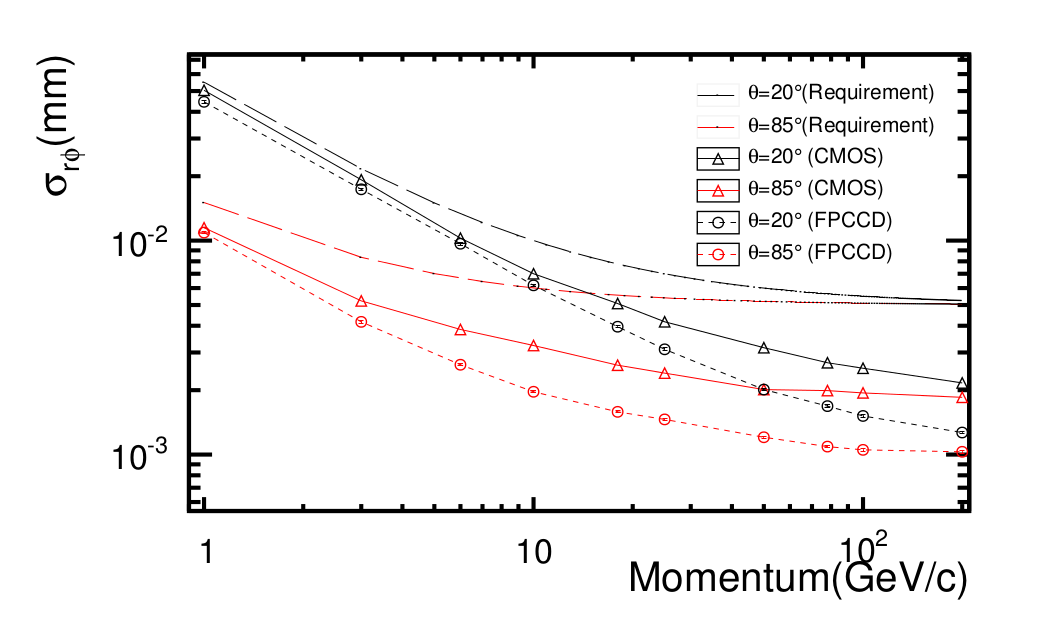
\includegraphics[scale=0.40]{./figures/sigmaIP_vs_p.png}
      \caption{R\'esolution sur le param\`etre d'impact du d\'etecteur de vertex de l'ILD pour deux angles de productions de particules diff\'erents. Ces r\'esultats sont bas\'es sur les caract\'eristiques du détecteur de vertex donn\'ees dans le tableau \ref{tab:caractVXD}. Deux options de capteurs sont \'etudi\'es : les CMOS (lignes pleines) et les FPCCD (lignes pointill\'ees). Les pointill\'es longs indiquent les spécifications requises.}
      \label{fig:sigmaIP}
    \end{center}
  \end{figure}
  
  \medskip
  
  Afin d'atteindre un tel param\`etre d'impact le d\'etecteur de vertex de l'ILD devra poss\'eder les caract\'eristiques suivantes : 

  \medskip
  
  \renewcommand{\labelitemi}{$\bullet$}
  \begin{itemize}
   \item Une r\'esolution spatiale sur les premi\`eres couches du VTX $\leq$ 3 $\mu m$
   \item Un budget de mati\`ere inf\'erieur \`a $0.15 \%$ $X_0$ par couche
   \item Une premi\`ere couche \`a environ 1.6 $cm$ du point d'impact.
   \item Un taux d'occupation inf\'erieur \`a quelques pourcents.
   \label{list:caracteristiques}
   \end{itemize}
  
  \medskip  

  La puissance consomm\'ee doit \^etre réduite afin de minimiser le syst\`eme de refroidissement et donc le budget de mati\`ere. Pour cela la structure en temps du faisceau peut \^etre mise \`a profit en mettant en veille les capteurs durant les périodes sans faisceau et en les rallumant durant les p\'eriodes où le faisceau est pr\'esent, c'est ce que l'on appelle le \textit{power-pulsing}. La tol\'erance aux radiations des capteurs est directement reli\'ee aux bruits de fond faisceau, qui comme nous l'avons vu pr\'ec\'edemment dominent le taux de radiations (voir section \ref{sect:beamstrahlung}). C'est particuli\`erement le cas pour la premi\`ere couche de d\'etection du d\'etecteur soumise aux plus fortes doses de radiations, les autres couches subissant de moins en moins les radiations caus\'ees par le bruit de fond induit par le faisceau. Ainsi, les capteurs devront r\'esister \`a une dose ionisante de l'ordre de 100 $kRad/an$ et \`a une fluence d'environ $10^{11} \, n_{eq}/cm^2$ (neutrons d'environ 1 $MeV$) par an.
  
  \medskip
  
  De plus, le bruit de fond faisceau, contraint le rayon minimum et la vitesse de lecture des premi\`eres couches. En effet, plus on se rapproche de la région d'interaction, plus la densit\'e surfacique d'impacts a tendance \`a augmenter. Deux solutions permettent de garder un taux d'occupation acceptable : une granularit\'e pour la premi\`ere couche amenant \`a une r\'esolution d'environ 3 $\mu m$ associ\'ee \`a une vitesse de lecture adapt\'ee pour un rayon minimum optimis\'e (CMOS) ou une plus forte granularit\'e associ\'ee \`a un temps de lecture plus important pour un rayon minimum optimis\'e (FPCCD). Si l'on ne compte pas les particules de beamstrahlung retrodiffus\'ees (retard\'ees en temps) vers le d\'etecteur de vertex, plus la vitesse de lecture augmente et plus le nombre d'impacts moyen par unit\'e de surface tend \`a diminuer. De plus, selon cette m\^eme condition, plus l'on s'\'eloigne de la r\'egion d'interaction, et plus la densit\'e surfacique d'impacts diminue. Lorsque l'on inclut les particules r\'etrodiffus\'ees et les particules bouclant \`a cause du fort champs magn\'etique ($3.5 \, T$), les variations sont plus complexes et des simulations sont n\'ecessaires afin d'estimer le taux d'occupation (voir chapitre \ref{chap:alignement}).
  
%   De plus, comme nous le verrons dans le chapitre suivant, \`a design \'egal, augmenter la vitesse de lecture revient \`a d\'egrader la r\'esolution spatiale atteignable sur l'un des axes du capteur. Optimiser la g\'eom\'etrie d'un d\'etecteur de vertex n'est donc pas chose facile, et des compromis doivent \^etre trouv\'es. Par exemple, le concept d'\'echelles double face permet de jouer sur les param\`etres des deux faces. La premi\`ere face pourrait ainsi \^etre optimis\'ee pour atteindre une r\'esolution spatiale de l'ordre de 3 $\mu m$ tout en ayant une vitesse de lecture plus faible que la seconde, optimis\'ee pour l'\'etiquetage temporel mais poss\'edant une r\'esolution moindre.
  
%   Cette fluence suppose que les neutrons r\'etro-diffus\'es depuis les points d'arrêts du faisceau sont suffisamment stopp\'es pour qu'ils ne contribuent que de façon minoritaire.

    \begin{figure}[!htb]
    \begin{center} 
      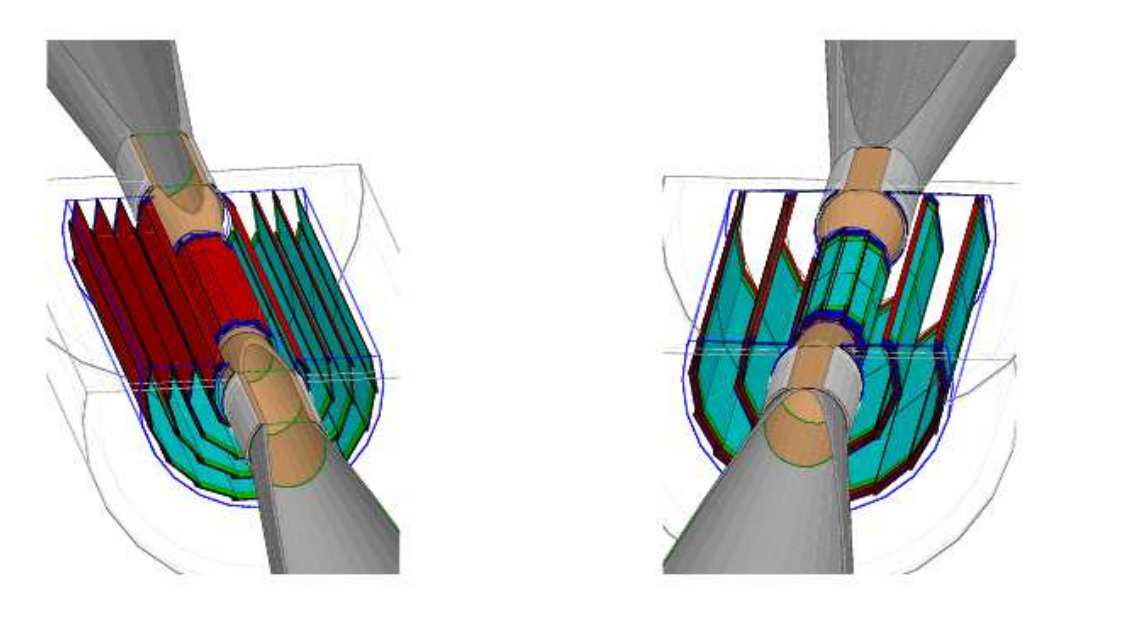
\includegraphics[scale=0.30]{./figures/options_VXD.png}
      \caption{Deux options pour le d\'etecteur de vertex. La principale avec 3 couches double face \`a droite, et l'option alternative avec 5 couches simple face \`a gauche.}
      \label{fig:optionsVXD}
    \end{center}
  \end{figure} 
  
  \begin{table}[h]
  \begin{center}
  \begin{tabular}{|l|l|l|l|l|l|} \hline
           & $R(mm)$ & $|z|(mm)$ & $|\cos(\theta)|$ & $\sigma(\mu m)$ & temps de lecture $(\mu s)$ \\ \hline \hline
  couche 1 &   16    &   62.5    &       0.97       &      2.8        &           50               \\
  couche 2 &   18    &   62.5    &       0.96       &      6.0        &           10               \\ \hline
  couche 3 &   37    &   125     &       0.96       &      4.0        &           100              \\
  couche 4 &   39    &   125     &       0.95       &      4.0        &           100              \\ \hline
  couche 5 &   58    &   125     &       0.91       &      4.0        &           100              \\
  couche 6 &   60    &   125     &       0.90       &      4.0        &           100              \\  \hline
  \end{tabular}
  \caption{Caract\'eristiques de l'option principale \`a 3 couches doubles faces pour le d\'etecteur de vertex.}
  \label{tab:caractVXD}
  \end{center}
  \end{table}
  
  \medskip
  
  Deux options pour la conception du d\'etecteur de vertex ont \'et\'e retenues. L'option principale consiste en un d\'etecteur constitu\'e de 3 couches cylindriques double face, alors que l'option alternative est bas\'ee sur 5 couches cylindriques simple face. Pour la premi\`ere option chaque \'echelle de chaque double couche est \'equip\'ee de capteurs sur ces deux faces, les deux faces \'etant s\'epar\'ees d'une distance d'environ 2 $mm$. Ainsi, pour chaque particule charg\'ee traversant le d\'etecteur de vertex, six points de mesure seront enregistr\'es. Les rayons des double couches sont compris entre 16 et 60 $mm$ et le budget de mati\`ere pour chaque double couche est d'environ 0.3 $\% \, X_0$ ce qui \'equivaut \`a un budget de mati\`ere pour une couche simple face de 0.15 $\% \, X_0$. Les caract\'eristiques de cette option sont list\'ees dans le tableau \ref{tab:caractVXD}. Elles sont bas\'ees sur des simulations et des \'etudes techniques r\'ealis\'es pour le \textit{DBD} de l'ILC. L'option alternative est bas\'ee sur 5 simples couches de d\'etection espac\'ees de fa\c{c}on équidistantes entre 15 et 60 $mm$. Ces deux options sont illustr\'ees en figure \ref{fig:optionsVXD}. 
  
  \medskip
  
%   On peut effectuer un calcul simple pour approximer le taux d'occupation des capteurs pr\'esent sur la premi\`ere face de la premi\`ere double couche. Comme vu plus haut le nombre d'impacts moyen par $cm^2$ et par croisement de faisceau est estim\'e \`a $\lesssim 8$. A titre d'illustration, prenons un facteur de s\'ecurit\'e et estimons ce nombre \`a environ 10 impacts par $cm^2$ et par croisement de faisceau. Un capteur d'environ $10^6$ pixels mesure environ 4 $cm^2$. Prenons alors une vitesse de lecture de 50 $\mu s$ et un nombre de pixels touch\'es par impact d'environ 5. Le nombre de croisements de faisceaux durant 50 $\mu s$ est d'environ $BXs = 50/0.552 \approx 90$. Le nombre de pixels touch\'es est alors d'environ : $N_{pix} = 10 \times 4 \times 5 \times BXs = 36000$. Ce qui pour $10^6$ pixels repr\'esente un taux d'occupation d'environ $3.6\%$. Pour un temps de lecture de 10 $\mu s$ on obtient un taux d'occupation environ 5 fois moins \'elev\'e soit environ $0.7 \approx 1.0 \%$. Un taux d'occupation de 1 \`a 2 $\%$ est tout a fait envisageable.
  
  \medskip
  
  Cette th\`ese a pour but d'\'etudier la valeur ajout\'ee des \'echelles double face en terme d'alignement. Mais avant de rentrer plus en d\'etail dans le sujet de l'alignement, nous allons \'etudier les capteurs CMOS d\'evelopp\'es dans le groupe \textit{PICSEL} et leurs caract\'eristiques. Ainsi, les chapitres suivants traiteront de l'optimisation des capteurs CMOS et des \'echelles de capteurs CMOS pour le d\'etecteur de vertex de l'ILC. Ceci nous donnera une base solide dans le but de construire une simulation num\'erique de ces capteurs CMOS, et de prototypes d'\'echelles double face. La voie sera alors ouverte pour l'\'etude de l'alignement de deux \'echelles double face d'une m\^eme couche, \`a l'aide des mini-vecteurs reconstruits sur chacune d'elle, en utilisant leur zone de recouvrement. Enfin, nous effectuerons une analyse plus d\'etaill\'ee du bruit de fond faisceau dans le dernier chapitre de cette th\`ese et nous en deduirons les nouveau temps de lecture pour les capteurs du d\'etecteur de vertex.
  
%   choix 5 couches simples faces ou 3 doubles faces (tableau des rayons des 
% couches, cf TDR) \\
%   Schéma 5 faces vs 3 doubles faces.
  

  
%   Description des différentes couches (résolution, tps de lecture, dissipation thermique, ...) \\
%   Échelles doubles faces de capteurs : caractéristiques \\
%   Conflit granularit\'e vs tps de lecture \\
%   -> parler de PLUME. \\
%   Pour tester tout ça -> Transition sur AIDA \\

% Limites du modele standard
% -->Pb non resolus avec le MS
% 
% Physique au dela du MS
% --> Description simple
% 
% Physique \`a l'ILC : globalement.
% --> comprendre le Higgs du MS.
%   --> Production
%   --> Detection
%   --> Mesure (Masse de recul)
%   --> Section efficace % /!\ (Partie saveur lourde) /!\
% --> Apres le MS
%   --> SuSy
%   --> Higgs non std
%   ...
%   
% ILC : description.
% --> Les bases.
% --> La Machine.
% --> Interactions faisceau-faisceau.
% --> ILD
% --> Reconstruction/Alignement ILD. (Particule Flow Algorithm)
% 
% \section{Au dela du mod\`ele standard : nouvelle physique}
% 
%   \subsection{Nouvelle physique}
%    
%    A mettre peut etre plus haut apres le  chapitre de th\'eorie sur le Higgs ;)
%    Au dela du modele standard ...
%    Supersym\'etrie. \\
%    Theorie Mond. \\
%    Grav Quat. a boucles \\
%    Th\'eorie des cordes. \\
%    ... \\
%    
%   \subsection{Acc\'el\'erateurs}
% 
%    Pour pouvoir decouvrir et mesurer plus pr\'ecis\'ement.
% \section{Physique ILC}
% \section{Physique des saveurs et d\'etecteur de Vertex}
% comparaison LHC ...